\documentclass[12pt,a4paper]{book}

%\usepackage{CJK} %使用CJK套件
\usepackage{url}
\usepackage{CJKutf8}
\usepackage{comment}
\usepackage{ucs}
\usepackage[utf8]{inputenc}
\usepackage{listings}
\usepackage{hyperref} % 最好保證 hyperref 是最後載入的 macro
\hypersetup{%
%  dvipdfmx,% 设定要使用的 driver 为 dvipdfmx
  dvips,% 设定要使用的 driver 为 dvipdfmx
  unicode={true},% 使用 unicode 来编码 PDF 字符串
  pdfstartview={FitH},% 文档初始视图为匹配宽度
  bookmarksnumbered={true},% 书签附上章节编号
  bookmarksopen={true},% 展开书签
  pdfborder={0 0 0},% 链接无框
  pdftitle={thinker in java 2nd edition},
  pdfauthor={},
  pdfsubject={java},
  pdfkeywords={java},
  pdfcreator={ps2pdf},
  pdfproducer={PDF 制作程序},% 这个好像没起作用?
}




\begin{comment}
\ctxfdef{\chapter}{\ctxfm}{\ctxfr}
\ctxfdef{\section}{\ctxfm}{\ctxfr}
\ctxfdef{\subsection}{\ctxfm}{\ctxfr}
\ctxfdef{\subsubsection}{\ctxfm}{\ctxfr}
\end{comment}

\usepackage{graphicx}
\usepackage{booktabs}
\usepackage[sf]{titlesec}
%\ctxfdef{\chapter}[\ctxfm]{\ctxfm}

% 照列原文
\usepackage{fancyvrb}
\usepackage{fancyhdr}
\pagestyle{fancy}

\fancyhf{}
\fancyhead[LE]{\leftmark}
\fancyhead[RO]{\rightmark}
\fancyfoot[CE,EO]{Thinking in Java}
\fancyfoot[RE,LO]{www.BruceEckel.com}
\fancyfoot[LE,RO]{\thepage}
\renewcommand{\footrulewidth}{0.4pt}


\fancypagestyle{plain}{%
\fancyhf{} % clear all header and footer fields
\fancyfoot[RO]{\thepage}
\fancyfoot[LE]{\thepage}
\renewcommand{\headrulewidth}{0pt}
\renewcommand{\footrulewidth}{0pt}}

\begin{document}

%\begin{CJK}{UTF8}{cwfsu} 
\begin{CJK}{UTF8}{cybercjk} 

\renewcommand{\contentsname}{目錄}
\renewcommand{\tablename}{表}
\renewcommand{\figurename}{圖}
\renewcommand{\listtablename}{表格目錄}
\renewcommand{\listfigurename}{圖目錄}
\renewcommand{\chaptermark}[1]{\markboth{第\ \thechapter\ 章\ #1}{}}
\renewcommand{\sectionmark}[1]%
%\titleformat{\chapter}[display]{\LARGE\sf}{第\ \thechapter\ 章}{0.2cm}{}
%{\markright{\thesection~ #1}}

\frontmatter
\tableofcontents
\listoftables
\listoffigures
\chapter[序言]{序言}\marginpar{\fbox{1}}
我想起我的兄弟Todd,他正從硬體領域大躍進到程式設計領域。
基因工程將是下一個大革命的戰場。

我們將擁有許多被設計用來製造食物、燃料、塑膠的各類微生物;這些微生物的出現,
可以免去污染,讓我們僅付出遠少於現今所付的代價,便足以主宰整個物質世界。
我原以為,這場革命規模之大,將使電腦革命相形見絀。

然而,後來,我發覺我犯了科幻作家所犯的同樣錯誤:對科技的迷失
(當然,這在科幻小說中屢見不鮮)。有經驗的作家都知道,故事的重點不在技術,
而在於人。基因工程無疑會對我們的生活造成極大衝擊,
但是我不確定它是否會阻礙電腦革命(電腦革命也帶動了基因工程的到來)
或至少說是資訊革命。所謂資訊,關注的是人際之間的溝通。是的,車子、鞋子、
尤其是基因治療,都很重要,但這些東西最終都和陷阱沒什麼兩樣。
人類與世界共處的方式,才是真正關鍵所在。而這其中,溝通居重要角色。

本書是一個例子。大多數人認為我很大膽、或者說有點瘋狂,因為我把所有材料都放上了
Web。「那麼,還有什麼購買理由呢?」他們這樣問我。 如果我的性格保守謹慎一些,
我就不會這麼做了。但是我真的不想再用同樣老舊的方式來撰寫一本新的電腦書籍。
我不知道會發生什麼事,但事實證明,這是我對書籍所做過的最棒的一件事。

首先,人們開始把校正結果送回。這是個讓人驚嘆的過程,因為人們仔細端詳每個角落、
每個縫隙,揪出技術上和文法上的種種錯誤,讓我得以更進一步消除所有毛病,
而這些毛病原本是被我遺漏未察的。人們往往對這種作法表示驚恐,
他們常常說「唔,我不確定我這麼做是否過於吹毛求疵...」,然後扔給我一大堆錯誤。
我發誓,我自己從未曾察覺這些錯誤。 我很喜歡這種群體參與的過程,
這個過程也使這本書更加獨特。

但是,\marginpar{\fbox{2}} 接著我開始聽到「嗯,很好。
整個電子版都能夠放到網絡上實在不錯,可是我希望擁有出版商印出來的、
裝訂成冊的紙本。」我曾經努力讓每個人能夠更輕鬆地以美觀的方式把它印出來,
但這麼做似乎還是無法滿足要求此書付梓的強大呼聲。
大部份人都不希望在電腦螢幕上讀完一整本書,也不希望總是拖著一捆捆的紙。
即便這些紙張印刷再美觀,對他們來說也不具半點吸引力
(而且我想雷射印表機的碳粉也不便宜)。即使是電腦革命,似乎也難以削減出版商的生意。
不過,某個學生提出了一種看法,他認為這也許會成為未來的一種出版模型:先在
Web 上公開書籍內容,只有在吸引了足夠關注時,才考慮製作紙本形式。目前,
絕大多數書籍都不賺錢,這種作法或許可以讓整個出版產業更有利潤一些。

這本書以另一種形式對我產生了啟迪。一開始我把Java 定位在
「只不過是另一個程式語言」。從許多角度看的確如此。但是隨著時間流逝,對Java
的學習日深,我開始明白這個程式語言的最根本目的,和其他我所見過的程式語言有著極大的不同。

程式設計,就是對複雜度的控管。複雜度包括:待解問題的複雜度和底層機器的複雜度。
因為有著這樣子的複雜度,所以大多數程式開發專案都失敗了。到目前為止,
所有我所知道的程式語言,沒有一個竭盡所能地將主要設計目標鎖定在
「克服程式發展與維護過程中的種種複雜度」上\footnote{在此第二版中,
我要收回這句話。我相信,Python 語言極為逼近這個目標。請參考 www.Python.org。}。
當然,許多程式語言當初設計時也曾將複雜度考慮進去,
但是總有被視為更本質的問題混雜進來。毫無疑問,
那些問題也都是會讓語言使用者一籌莫展的問題。舉例來說,C++回溯相容於
C(俾使熟悉C 的程式員得以比較\marginpar{\fbox{3}}輕鬆地跨越門檻),
並具備高執行效率的優點。這兩個特性都是大有幫助的目標,並擔負起
C++成敗的重責大任。不過,兩者也帶來了額外的複雜度,使得某些專案無法完成。
(通常你可以將此點歸罪於程式開發人員或管理人員,
不過如果某個語言可以協助我們捕捉錯誤,何樂不為?)
Visual Basic(VB)是另一個例子,它被BASIC 這個「其實不以擴充性為設計目標」
的語言侷限住,使得所有強硬堆累於VB 之上的擴充功能,
都造成了可怕至極且難以維護的語法。Perl 也回溯相容於Awk、Sed、
Grep、以及其他諸般它想取代的Unix 工具,於是衍生出諸如「能寫卻不能讀」的程式碼
(write-only code)這種指責(意思是,寫完數個月之後,你便無法閱讀它)。另一方面,
C++、VB、Perl、Smalltalk 之類的程式語言,都在複雜度議題上有著相當程度的著墨,
十分成功地解決了某些類型的問題。

當我了解Java 之後,最叫我感動的,莫過於Java 似乎把「為程式員降低複雜度」
做為一個堅定的目標。就好像是說:『我們的唯一考量,
就是要降低穩固程式碼的產生時間和困難度』。早期,
這個目標只開花結果於程式碼的撰寫上,
但這些程式碼卻無法執行得很快(雖然目前有許多保證, 承諾
Java 總有一天能夠執行得多快多快)。但是Java 的確出人意表地大幅縮短了發展時間;
比起發展等價的C++ 程式來說,大概只需一半或甚至更少時間。光是這個結果,
就足以省下驚人的時間與金錢。不過,Java 並未停止腳步。Java 繼續將多執行緒、
網絡程式設計等等複雜而益形重要的工作包裝起來。透過語言本身的性質以及程式庫
(libraries),有時能夠使這些工作變得輕而易舉。最後一點,
Java 著眼於某些有著極高複雜度的問題:跨平台程式、動態程式碼改變、安全議題,
其中每一個問題都能夠套用在整個複雜度頻譜的任何一點上。
所以儘管有著眾所周知的效率問題, Java 帶來的保證卻是很棒的:
可以讓我們成為具有高生產力的程式開發者。

我所見到的種種巨幅改變,有一些是發生在Web 身上。
網絡程式設計一直都不是件簡單的事,但是Java 把它變簡單了
(而Java 語言設計者仍舊繼續努力使它變得更簡單)。網絡程式設計所討論的,
便是讓我們以更有效率、成本更低的方式,和其他人通訊,超越舊式電話媒介
(單是電子郵件\marginpar{\fbox{4}}便已經革命性地改變了許多事情)。
當我們能夠在與他人溝通這件事情上著力更多,神奇的事情便會開始發生,
或許甚至比基因工程所許諾的遠景,更讓人感到神奇。

透過所有努力 - 程式開發、團隊開發、使用者介面的打造(讓程式可以和使用者互動)、
跨平台的執行、跨Internet(網際網、互聯網)通訊程式開發的大量簡化 - Java 擴展了
「人際之間」的通訊頻寬。我認為,
通訊革命的成果或許不應只是圍繞在傳輸頻寬提高後所產生的效率上打轉;
我們將會看到貨真價實的革命,因為我們能夠更輕鬆地和其他人溝通:
可以是一對一的形式、可以是群體通訊的形式、也可以是和全地球人通訊的形式。
我曾經聽人主張,接下來的革命會是一種全球意志的形成,
來自於足夠數量的人們和足夠數量的相互聯繫。Java 可能是、
也可能不是點起這把撩原之火的星焰,但至少存在著可能。這使我覺得,
這個語言的教學是一件有意義的事。


%\addcontentsline{toc}{section}{第二版序}
\section{第二版序}

關於本書的第一版,人們給了我許多許多精彩的意見。我當然對此感到非常愉快。
不過有時候讀者也有抱怨。一個常常被提起的抱怨便是:這本書太大了。對我來說,
如果「頁數過多」的確是你唯一的怨言,那真是一個讓人無言以對的責難。
(這讓人想起奧地利皇帝對莫札特作品的非難: 『音符太多了!』
當然我並不是將自己拿來和莫札特相提並論)我只能夠假設,
這樣的怨言出自於一個「被塞進太多Java 語言的廣闊內容,
而還未看過其他相同主題的書籍」的人。就拿我最喜歡的一本參考書來說好了,
它是Cay Horstmann 和Gary Cornell 合著的《Core Java》(Prentice - Hall 出版),
其規模甚至大到必須拆成兩冊。儘管如此,在這一 (第二) 版中,我努力嘗試的事情之一,
便是修剪過時的內容,或至少不是那麼必要的內容。這麼做我覺得很自在,
因為原先內容仍然擺在網站 www.BruceEckel.com 上,
而且本書所附光碟中也有第一版的內容。

如果你想取得原本內容,\marginpar{\fbox{5}} 沒有任何問題,
這對作者而言也是一種欣慰。舉個例子,您可能會發現第一版的最後一章「專案
(Projects)」已不復存在;有兩個專案被整合到其他章節裡頭,
因此剩餘部份也就變得不再適合存在。同樣的,「設計樣式
(Design Patterns)」這一章的內容變得更豐富了,因此也獨立成冊了
(可自我的網站下載)。基於這些原因,本書理應變得苗條一些。

事實卻非如此。

最大的問題是,Java 語言本身仍在持續發展當中,
企圖為所有可能用到的東西提供標準化介面,因此 API 的數量不斷擴增。所以就算看到
JToaster 這樣的API 出現,我也不會吃驚) (譯註:toaster 是烤麵包機,JToaster
意指標準化的烤麵包機類別。連烤麵包機都有標準類別,藉此誇飾 Java 2
所涵蓋的類別的廣泛程度)。「涵蓋所有API」似乎逾越本書範圍,應該交給其他作者完成,
但儘管如此,仍然有某些議題難以略去。伺服端 Java (主要是 Servlets 和
Java Server pages,JSPs)便是這些議題中涵蓋最廣的一個。伺服端 Java 無疑為
WWW 的諸多問題提供了出色的解決方案。
尤其當我們發現「現存許多不同的 Web 瀏覽器平台,
無法提供一致的用戶端程式開發」時,更顯其重要性。此外
Enterprise Java Beans(EJBs)的問世,也讓人們希望更輕易地發展資料庫連結、
交易處理、安全考量。這些問題在本書第一版本中通通被放進「網絡程式設計」一章。
本版則改用了一個對每個人來說都愈來愈不可或缺的名稱:「分佈式計算」。
你還會發現,本書同時也將觸角伸至Jini(讀作genie,這真的只是個名字,
不是什麼字首縮寫)的概要性說明。
此一尖端技術讓我們重新思考應用程式之間的接駁形式。當然,本書所有內容都已改用
Swing 這個 GUI 程式庫。再次提醒你, 如果你想要取得原有的 Java 1.0/1.1 書籍內容,
可自 www.BruceEckel.com 免費下載
(網站上同時也包含第二版書附光碟的內容;新的材料還會陸續增加)。

本書不但新增的少數 Java 2 語言特性,也徹頭徹尾地翻修了一遍。
最主要的改變是第九章的群集(collection),我將重點改放在Java 2 的群集,
並修繕本章內容,更深入鑽進某些更重要的群集議題之中,尤其是對 hash function
(雜湊函式)運作方式的討論。此外還有其他一些變動,
包括重寫\marginpar{\fbox{6}}第一章,抽掉部份附錄以及我認為新版不再需要的內容。
整體而言,我重新審閱所有內容,移去第二版中不再需要的部份
(但仍保留它們的電子版於我的網站上),並將新的更動加入,
然後儘可能改進我能夠改進的所有地方。這種大變動是由於語言本身持續有所變化 -
即使不再像以前那麼大刀闊斧。以此觀之,毫無疑問,本書還會有新版面世。

對那些吃不消本書厚度的讀者們,我向你們致歉。不管你們是否相信,
我真的傾盡全力地想辦法讓這本書更輕薄。儘管體積依舊龐大,
我認為有其他令你滿足的方式。本書也有電子版形式
(不論是從網站取得,或是從本書所附光碟取得),你可以帶著你的筆記電腦,
把這本電子書放進去,不增加絲毫重量。如果你希望更輕便地閱讀,
也可以找到四處流傳的 Palm Pilot 版
(有人跟我說,他總是躺在床上以Palm 閱讀本書內容,並打開背光裝置
(譯註:Palm PDA 上一種用於夜間燈光不足時的顯示模示)以免打擾太太。
我想這應該有助於讓他早點進入夢鄉)。如果你一定得在紙上閱讀,
我知道有些人一次印出一章,然後帶在公事包裡頭,在電車上閱讀。
\subsection{Java 2}
本書撰寫之際,Sun 即將發行Java Development Kit(JDK)1.3,並預告 JDK 1.4
將有的更動。雖然這些版本的主號碼還停留在1,但是 ``Java2'' 卻是
JDK 1.2 及其後續版本的標準名稱。這突顯了介於「老式Java」
(其中有許多本書第一版中抱怨過的缺點)與新版本之間的重大差異。
在這些更新更精進的新版本中,缺點變少了,加入了許多新特性和美妙的設計。

本書是為Java2 而寫。能夠擺脫過去的陳舊內容,重新以更新的、更精進的語言來寫作,
這個事實給我憑添許多樂趣。舊有的資訊依舊存於網站上的第一版電子書及光碟中,
如果你使用Java 2 之前的版本,便可拿它們來參考。由於每個人都可以自
java.sun.com 免費下載JDK,所以就算我\marginpar{\fbox{7}}以 Java 2 撰寫本書,
也不會讓讀者為了升級而付出金錢。

不過,還是有點小麻煩,這是因為 JDK 1.3 提供了某些我想用到的改進功能,
而目前 Linux 上正式發行的版本只到JDK1.2.2 。Linux ( 見 www.Linux.org) 是個和
Java 關聯極深的重要開發環境。Linux 正以極高的速度成為最重要的伺服器平台,快速、
穩定、強固、安全、容易維護, 而且免費,的確是電腦史上的革命
(我不認為可以在過去任何工具上同時看到這些特色)。 Java
則在伺服端找到了極為關鍵的利基所在,也就是 Servlets 這個為傳統 CGI
程式設計帶來巨大改進效應的新技術(本主題含括於「分佈式計算」一章)。

所以,雖然我想完全使用最新功能,但是讓每一個程式都在Linux 上順利編譯,
對我而言至關重要。當你解開本書原始碼檔案,並在Linux 上以最新的 JDK 進行編譯,
你會發現所有程式應該都能夠順利完成。然而你會看到我四處放置的有關 JDK 1.3
的註記。

\section{書附光碟}
這個(第二)版本提供了一份紅利:附於書後的光碟。
過去我不想將光碟放在我所撰寫的書籍後面,原因是我覺得,為了大小僅數百
K bytes 的原始碼,用了那麼大一片光碟,實在說不過去。
我傾向於讓讀者從我的網站下載這些東西。但是現在,你看到了,
本書所附的光碟大有不同。

這片光碟當然包含了本書所有原始碼,此外還包含本書完整內容的多種電子形式。
我最喜歡HTML 格式,不但速度快,索引也十分完備 - 只要在索引或目錄上按下某個項目,
馬上就可以跳到你想閱讀的地點。

整張光碟有著超過 300 Mega 的滿滿內容,
是一個名為《Thinking in C Foundations for C++ \& Java》的全多媒體課程
。我原本委託 Chuck Allison 製作這張光碟,是希望做成一個獨立產品。
但後來決定將它放在\marginpar{\fbox{8}} 《Thinking in C++》 和
《Thinking in Java》 兩本書的第二版中,因為持續有一些尚未具足
C 語言背景的人來上我的研討課程,他們認為:『我是個聰明的傢伙,我不想學
C,只想學 C++或 Java,所以我直接跳過C,進到 C++/Java 裡頭。』加入研討班後,
這些人才逐漸了解,認識基本的 C 語法,是多麼重要。將光碟片納入本書,
我便可以確信,每個人都能夠在準備充裕的情形下參加我的研討課程。

這份光碟同時也讓本書得以迎合更多讀者的喜好。
即使本書第三章「程式流程的控制」已經涵蓋了取自 C 核心部份的
Java 相關語法,這張光碟仍然是一份很好的導引。
它所假設的學員基礎也比本書寬鬆許多。希望這張光碟的附上,
能夠使愈來愈多的人被帶領進入Java 程式設計的大家庭。

%\addcontentsline{toc}{section}{第二版序}
\chapter{簡介 (Introduction)}\marginpar{\fbox{9}}
Java,一如人類所使用的任何一種自然語言,提供的是意念表達的機制。
如果使用恰到好處,那麼作為一種表達媒介,
當你打算解決的問題益形龐大複雜,解法益形簡易而富彈性。

你不能僅僅將Java 看成某些特性的集合- 這些特性之中某些被支解而被獨立對待時,
將不具絲毫意義。只要你心中存有「設計」念頭,而非單單只是撰碼,
那麼便可以整體性地運用Java 的所有組成。如果想以這種方式來了解
Java,你還必須了解其衍生問題,以及在一般情況下其程式設計過程所衍生的問題。
本書所討論的是程式設計的問題、它們之所以成為問題、以及
Java 採取的解決方案。因此,我在各章之中所描述的各種特性,
其建構基礎皆是「我所看到的此一程式語言,在解決特定問題時的方式」。
透過這種方式,希望能夠對你潛移默化,漸漸地讓
Java 式思考模式成為對你而言再自然不過的一件事。

我的態度始終一致:你得在腦中建立模型,藉以發展出對此程式語言的深層體會和洞悉;
如果你在某個問題上陷入思想泥沼,可將它饋入腦內模型,並推導答案。
\section{閱讀門檻}
本書假設你對編程(programming)一事有著某種程度的熟悉:
你已經了解程式是許多敘述句的集合,你已經明白副程式/函式/巨集的觀念,懂得諸如
``if'' 之類的流程控制敘述,以及諸如 ``while'' 之類的迴圈概念...等等。
你可以從許多地方學習到這些東西,例如用巨集語言來設計程式,或使用諸如
Perl 之類的工具來工作。只要你在編程上的境界能夠
「自在地以編程基本概念來編寫程式」,那麼你便可以閱讀本書。當然,本書對於
C 程式\marginpar{\fbox{10}}員而言,相對容易些,對C++程式員而言更是如此。
但如果你對這兩種語言毫無經驗,也不必妄自菲薄(但請懷著高度的學習熱忱。
本書所附的多媒體光碟,能夠帶領你快速學習對Java 而言必備的基本C 語法)。
我同時會引入物件導向程式設計(Object-Oriented Programming,OOP)
的觀念,以及Java 的基本控制機制。你會接觸到這一切,
並在第一個練習題中練習基本的流程控制敘述。

雖然書中有許多參考資料,介紹的是C/C++語言的特性,
但那並不是為了進行更深層的詮釋,而只是希望幫助所有程式員正確看待Java,畢竟
Java 是C/C++的後裔。我會儘量簡化這些參考資料,並解釋所有我認為
non - C/C++ 程式員可能不怎麼熟悉的部份。

\section{學習Java}

差不多就在我的第一本書《Using C++》( Osborne/McGraw-Hill , 1989)
面世的同時,我開始教授語言。程式語言的教學已經變成了我的職業。
1989 年起,我在世界各地,看到了昏昏欲睡的聽眾,有人帶著一張面無表情的臉孔,
困惑的神情兼而有之。當我開始對小型團體進行內部訓練時,
我在訓練過程中發掘到某些事實:即便是對我點頭微笑的學生,同樣困惑於許多議題。
我發現, 多年來在「軟體發展討論會( Software Development Conference)」上主持
C++(後來變成Java)專題的工作中,我和其他講師一樣,
潛意識裡想要在極短時間內告訴我的聽眾許多許多東西。由於聽眾的程度各有不同,
也由於我的教材呈現方式,最終無法顧及某部份聽眾。或許如此要求有些過份,
但因為我向來反對傳統授課方式(而且我相信對大多數人們來說,
反對的理由是來自於厭倦),所以我試著讓每個人都加速前進。

一度,我以十分簡短的方式做了許多不同風格的演出。最後,我結束了實驗和迭代
(iteration,一種在Java 程式設計中也會用到的技巧)」的學習歷程。
我根據授課經驗所學來的事物(它讓我可以長時間快樂教學),發展出一套課程。
這套課程採用分離並極易融會貫通的數個步驟來處理學習上的問題,
並採取動手實踐的研討形式(這是最理想的學習方式)。
在其\marginpar{\fbox{11}}中,我為每一小部份課程內容設計了多個練習題。
現在我將此一課程置於開放的 Java 研討課程內,你可以在
www.BruceEckel.com 網站上找到這份研討課程的內容。
(這個研討課程的簡介也可以在書附光碟中取得。上述網站也可以找到相關資訊。)

我從各個研討班獲得許多回饋訊息。
在我認為我的這份課程材料足以成為一份正式的教學工具之前,
這些回饋訊息對於我的課程材料的更動和調整,助益良多。儘管如此,
本書絕不能以一般的研討課程筆記視之 - 我試著在這些書頁中放入儘可能多的資訊,
並將這些資訊加以結構化,藉以引領你平順地前進至下一個討論主題。最重要的是,
本書是為那些孤單面對一個全新語言的讀者而設計。

\section{目標}
就像我的前一本書《Thinking in C++》一樣,
這本書結構性地環繞著程式語言教學引導上的過程。
我的原始動機是希望創造一些材料,使我可以將自己在研討課程中採用的風格,
融於程式語言教學之中。當我安排本書章節時,
我的思考方式就像思考「如何在研討班上一堂好課」一樣。我的目標是,
切割出可以在合理時數中教完而又容易被吸收的材料,並附帶適合於教室內完成的習題。
以下是本書的目標:
\begin{enumerate}
\item 一次呈現一個階段的題材,讓你可以在移至下一課題之前,輕鬆消化每個觀念。
\item 範例儘可能簡短、單純。
但是這麼一來便會在某種程度上遠離了真實世界的問題處理方式。儘管如此,我發現,
對初學者而言,詳盡理解每個範例,所帶來的愉悅勝過於了解它所能解決的問題範圍。
能夠在教室中吸引學習者興趣的程式碼,數量十分有限,因此我無疑得承受諸如
「使用玩具般的小例子」的種種批判,
但我還是滿心歡喜地接受任何可以為教學帶來益處的形式。
\item 謹慎安排諸般特性的呈現順序,\marginpar{\fbox{12}}
讓你不致於突兀地碰觸到任何未曾見過的內容。
萬一在某些情形下無法達到此一理想,我會提出一些簡要的引導。
\item 只給你那些「我認為對你了解此一程式語言而言十分重要」的內容,
而非將我所知道的一切都倒給你。我相信「資訊重要性的階層順序」的確存在,
某些題材對百分九十五的程式員來說或許沒有必要,這些資訊往往只會混淆他們的觀念,
並加深他們對此語言的複雜感受而已。舉個 C 語言的例子好了,
如果你能清楚記得運算子優先序 (operator precedence),
撰寫出精巧的程式碼想必輕而易舉。但這麼做卻有可能造成讀者、維護者的困惑。所以,
忘了運算子優先序吧!在任何可能混淆的地方使用小括號不就得了。
\item 讓每一節內容有足夠的焦點,縮短授課和練習時段之間的空檔。
這麼做不僅為了讓聽眾的心態更為主動,融入「自己動手做」的研討氣氛,
而且也讓讀者更具成就感。
\item 讓你始終踏在紮實的基礎上,透過對各課題的充份了解,
面對更困難的作業和書籍。
\end{enumerate}

\section{線上說明文件 (Online documentation)}
從Sun Microsystems 取得的Java 程式語言及其程式庫(可免費下載),
皆附有電子文件,使用Web 瀏覽器即可閱讀。幾乎所有
Java 編譯器廠商也都提供了此份文件,或是等價的文件系統。大部份
Java 書籍也都提供此份文件的複製品。所以,除非必要,本書不會重述其內容,
因為對你而言,使用 Web 瀏覽器來找尋 classes 的說明,比遍尋全書來得快多了
(更何況線上說明文件的版本可能更新)。只有當有必要補充線上文件之不足,
使你得以理解特定範例時,本書才會提供classes 的各種額外描述。 


\section{章節組織}\marginpar{\fbox{13}}
設計本書時,有一個念頭長在我心:人們面對Java 語言的學習路線。
研討班學員所給的回饋訊息幫助我了解哪些困難部份需要詳加闡述。在那些「太過燥進、
一次含入太多主題」之處,我也透過教材的呈現而一一明白:
如果企圖包含許多新主題,就得全部說明清楚,因為新東西很容易造成學生的困惑。
基於這個原因,我儘可能每次只講一小段主題,避免生出太多困擾。

因此,我的目標便是每一章只教授單一主題,或是一小組相關主題,
儘量不和其他主題有所牽扯。如此你便得以在前進至下一主題前,
完全消化目前知識背景中的所有題材。 以下就是本書各章的簡要描述,
它們分別對應於我的研討班各授課時程和練習時段。

\begin{description}
\item[第 1 章:] 物件導論(Introduction to Objects)
本章提供物件導向程式編寫(object oriented programming)
的概論性介紹,包括最基本問題的回答,例如物件(object)
是什麼、介面(interface)與實作(implementation)、抽象
(abstraction)與封裝(encapsulation)、訊息(messages)
與函式( functions ) 、繼承( inheritance ) 與合成
(composition),以及最重要的多型(polymorphism)。
你也可以概要了解物件生成時的諸般問題, 像是建構式
(constructors)、物件的生命、物件被建立後置於何處、神奇的垃圾回收器
(garbage collector,當物件不再被使用時能夠加以清理回收)。其他相關議題也有討論,
包括異常處理 (exception handling)、多執行緒(multithreading)、網絡、
Internet 等等。你會看到是什麼東西使得Java 卓越出眾,
是什麼原因使得Java 如此成功,你也會學到物件導向的分析概念和設計概念。

\item[第 2 章:] 萬事萬物皆物件(Everything is an Object)
本章引領你開始撰寫第一個Java 程式。因此所有最基本的概觀都必須在這裡教給你,
包括:object reference(物件引用)\marginpar{\fbox{14}}觀念、物件產生方式、
基本型別(primitive types)與陣列 (arrays)、物件的生存空間(scoping),
物件被垃圾回收器回收的方式、如何在Java 中讓每樣東西成為新的資料型別
(class)、如何建立你自己的classes。此外還包括:函式、引數、回傳值、名稱可視性、
自其他程式庫取用組件 (components)的方式、關鍵字 static、註解、內嵌文件。
\item [第 3 章:] 控制程式流程(Controlling Program Flow)
本章首先討論的是Java 引自C/C++ 的所有運算子 ( operators ) 。
此外你會看到運算子的共通缺點、轉型 (casting)、型別晉升 (promotion)、運算優先序。
然後介紹基本流程控制,這是幾乎每一個程式語言都會提供的機制:
if-else 分支選擇、for/while 迴圈結構、以 break 和 continue
跳脫迴圈;其中當然包括了Java 的標註式(labeled)break 和標註式 continue (這是為了
Java 不再提供goto 而設計),以及 switch/case 選擇動作。雖然大部份特性和 C/C++
相同,但亦有些許差異存在。此外,所有範例皆以Java 撰寫,因此你可以清楚看到
Java 的程式風格。
\item [第 4 章:] 初始化與清理(Initialization \& Cleanup)
本章一開始先導入建構式(constructor)的概念,它用來保證初始化動作的順利進行。
建構式的定義會牽扯到函式重載 (function overloading) 觀念
(因為你可能同時需要多個建構式)。接著便是清理過程的討論,
這個過程的字面意義總是比實際簡單得多。正常情形下當你用完一個物件,
什麼也不必操心,垃圾回收器最終會執行任務,釋放該物件所配置的記憶體。
我會探討垃圾回收器及其本質。最後我們近距離觀察自動化的成員初值設定、
自定的成員初值設定、初始化順序、 static (靜態)初始化、以及 array 的初始化。
這些細微的物件初始化動作的探討,為本章劃上美好句點。

\item [第 5 章:] 隱藏實作細目(Hiding the Implementation)\marginpar{\fbox{15}}
本章討論程式碼的封裝,並解釋為什麼程式庫中某些部份被公諸於外,
某些部份卻被隱藏起來。一開始我們先檢視兩個關鍵字:package 和 import,
它們在檔案層次上進行封裝,並允許你打造 classes libraries。
接著探討目錄路徑和檔案名稱的問題。最後檢視 public、private、protected
等數個關鍵字, 並引介 ``friendly'' (友善的)存取動作,
以及不同情境下所使用的各種存取權限的意義。
\item [第 6 章:] 重複運用classes(Reusing Classes) 繼承 (Inheritance)
幾乎是所有物件導向程式語言的標準配備。它讓我們得以使用既有的 classes,
並得為它加入額外功能 (而且還可以改變,這是第七章的主題)。
繼承通常用於程式碼的重複運用(reuse):讓base class 保持不變,只補上你想要的東西。
不過,要想藉由既有的 classes 來製造新的 class, 繼承並非唯一途徑。
你也可以運用所謂的「複合」 (composition),將物件嵌入新的 class 內。
你可以在本章學到如何以 Java 的方式達到重複運用程式碼的目的,並學會如何應用。
\item [第 7 章:] 多型(Polymorphism) 多型,物件導向程式設計的基石。
如果只靠自我修練,你或許得花九個月的時間才能夠體會其奧秘。透過小而簡單的範例,
你將看到如何以繼承機制建立一整個族系的型別,並透過共同的 base class,
操作同一族系中的物件。Java
的多型機制允許你以一般性的角度看待同一族系的所有物件。
這意謂大部份程式碼不至於過度倚賴特定型別資訊,於是程式更易於延伸,
並使程式的發展與原始碼的維護更加簡單,更不費力。
\item [第 8 章:] 介面(Interfaces)與內隱類別(Inner Classes)
Java 提供「建立重複運用關係」的第三種形式:interface,
那是物件對外介面的一個純粹抽象描述。interface 不僅將抽象類別
(abstract class)發揮到極致,由於它允許你建立某種 class,可向上轉型
(upcast)至多個base classes,所以它提供了類似 C++「多重繼承
(multiple inheritance)」的變形。\marginpar{\fbox{16}}
inner classes(內隱類別)看起來似乎是個簡單的程式碼隱藏機制:只不過是將
class 置於另一個class 之內而已。但其實不僅於此,它知曉
surrounding class(外圍類別)並可與之溝通。雖然 inner classes
對大多數人而言是一個全新觀念,需要花上一些時間才能無礙地利用它從事設計,但
inner classes 的確可以讓程式碼更優雅、更澄淨。
\item [第 9 章:] 物件的持有(Holding your Objects)
一個程式如果只是擁有帶著已知壽命的固定數量的物件,這種程式其實是相當簡單的。
一般來說,你的程式會在不同時間點產生新物件,
而這些時間點只有程式執行之際才能確定。此外,除非處於執行期,
否則你可能無法知道你所需要的物件數量,及其確切型別。為了解決一般化的程式問題,
你必須有能力在任何時間、任意地點,產生任意數量的物件。本章深入探討 Java 2
所提供的容器程式庫(container library),讓你得以妥善保存你所需要的物件。
我的討論包括最簡單的 arrays (陣列),以及 ArrayList、HashMap 之類的複雜容器
(或說資料結構)。
\item [第 10 章:] 透過「異常」處理錯誤(Error Handling with Exceptions) 
Java 的基本設計哲學是,不允許「會造成損害」的程式碼執行起來。編譯器會儘可能捕捉
(catches)它所能捕捉的錯誤,但有時候某些問題 -
不論是程式員引起或程式正常執行下自然發生 - 只能夠在執行期被偵測、被處理。
Java 具備了所謂的異常處理機制 (exception handling),
可用來處理程式執行期引發的種種問題。本章討論了try 、catch、throw、 throws、
finally 等關鍵字在 Java 中的運作方式,並說明何時才是擲出
(throw)異常的最佳時機,告訴你捕捉到異常時該如何處理。此外你也會看到
Java 的標準異常,學習如何建立自定異常,並知道在建構式 (constructors)
中觸發異常時會發生什麼事,以及異常處理程序(exception handlers)的放置方式。

\item [第 11 章:] Java 的I/O 系統(The Java I/O System)\marginpar{\fbox{17}}
理論上你可以將程式劃分為三部份:輸入(input)、處理 (process)和輸出 (output)。
這意謂 I/O(輸入和輸出) 在此一方程式中佔了極大比重。本章可以讓你學到
Java 的諸般類別,讓你進行檔案、記憶體區塊、主控台(console)的資料讀取和寫入。
本章也會提及介於「傳統I/O」和「全新 Java I/O 」之間的差異。
此外本章也會檢視「將物件串流化 (streaming)」
(俾使物件得以被置於磁碟,或於網絡上傳遞)的過程,並討論如何將其重構
(reconstructing)。這些都是透過 Java 的「物件次第讀寫」(object serialization)
機制達成。當然,用於Java 保存檔(Java ARchive,JAR)格式的
Java 壓縮類別庫,也會在本章介紹。
\item [第 12 章:] 執行期型別辨識(Run-Time Type Identification)
當你僅有某物件的基礎類別的reference 時,Java 的執行期型別辨識
(RTTI)機制可讓你找出該物件的確切型別。通常你應該會想要刻意忽略物件的確切型別,
讓 Java 的動態繫結 (dynamic binding)機制(亦即多型,polymorphism)
負責展現特定型別應有的特定行為。不過有時候,當你僅有某物件的基礎類別的
reference,而能進一步知道該物件的確切型別, 可帶來很大用處。
通常此一資訊讓你得以更高效率地執行某些特定動作。本章說明:(1)何謂 RTTI,
(2)RTTI 的使用方式,(3)不該使用RTTI 時,應如何避免使用。本章也介紹了 Java 的
reflection 機制。
\item [第 13 章:] 建立視窗和 Applets Java 所附的 Swing GUI library,
是一組可攜性高的視窗相關類別程式庫。此處所謂的視窗程式,
可以是網頁內嵌小程式 (applets),也可以是獨立的應用程式 (applications)。
本章內容包含Swing 的簡介和WWW applets 的開發。同時也介紹極重要的 JavaBeans
技術 - 它是所有快速應用軟體開發工具(Rapid-Application Development,RAD)的根本。

\item [第 14 章:] 多執行緒(Multiple Threads) \marginpar{\fbox{18}}
Java 提供了一些內建機制,使得單一程式內可同時並行多個被稱為「執行緒
(threads)」的子工作(但除非你的機器裝載多顆處理器,
否則這種運作方式只是形式而已)。雖然任何地方都可以應用執行緒,
但最主要還是應用於需要高度互動能力的使用者介面上。舉個例子,
雖然還有一些處理動作正在進行,但使用者可以不受阻礙地按下按鈕或輸入資料。
你將在本章看到 Java 多執行緒的語法和語義。
\item [第 15 章:] 分佈式計算(Distributed Computing)
當你開始想要撰寫運行於網絡上的程式時,一時間好像所有的 Java
特性和類別庫都一起湧現。本章探討網絡及 Internet 的通訊問題,以及 Java
提供的相關 classes。本章也介紹了重要的 Servlets 和 JSPs 觀念
(兩者皆用於伺服端程式設計),以及 Java 資料庫連結機制
( Java Database Connectivity , JDBC ) 、遠端函式調用
( Remote Method Invocation, RMI)等技術。最後還介紹了 JINI、JavaSpaces、
Enterprise JavaBeans(EJBs)等的最新技術。
\item [附錄A:] 物件的傳遞和回傳(Passing \& Returning Objects) Java
允許你和物件溝通的唯一方式是,透過 reference 達成。
所以,將物件傳入函式內以及函式將物件回傳,便存在著某些有趣的結果。
這份附錄說明,當你將物件移入函式,或將物件自函式移出時需要知道哪些事情,
才能妥善管理這些物件。本附錄也為你介紹 String class
如何使用另一種截然不同的手法來解決問題。
\item [附錄B:] Java 原生介面(The Java Native Interface, JNI) 全然可攜的
Java 程式有某些致命缺點:執行速度慢、無法存取特定平台上的服務。
一旦你確切知道你的程式的執行平台,\marginpar{\fbox{19}}
大幅提升某些動作的執行速度是極有可能的 - 只要透過所謂的原生函式
(native methods )即可。原生函式係以另一種語言 (目前僅支援C/C++) 寫成。
這份附錄為你提供足夠的入門引導,讓你能夠寫出「和
non-Java 程式相接連」的簡單程式。
\item [附錄C:] Java 程式設計守則(Java Programming Guidelines)
本附錄提供許多建議,幫助你進行較低層次的設計和撰碼工作。
\item [附錄D:] 推薦讀物(Recommended Reading) 本附錄列出我所知道的
Java 書籍中格外有用的名單。
\end{description}


\section{習題}
研討班的經驗使我察覺,簡單的練習對於學生所需要的完整理解有著超乎尋常的效果。
因此每章末尾我都安排了一些習題。
大多數習題都夠簡單,
使你得以在指導者從旁協助的情況下,以合理的時間完成。
這可確保所有學生都順利吸收了教材內容。某些習題難度較高,
以免經驗豐富的學生心生厭倦。多數題目都可以在短時間內解決,
並可用來檢驗所學以及鍛練自己。某些題目具有挑戰性,但其中並沒有難度很高者 -
我想你應該會自己找到這樣的題目,或者很有可能它們會自動找上門來。

某些經過挑選的習題有電子檔解答,收錄於《The Thinking in Java
Annotated Solution Guide》,僅須小額付費即可自 www.BruceEckel.com 下載。
\section{多媒體光碟(Multimedia CD ROM)}
本書有兩張相關的多媒體光碟。第一張光碟《Thinking in C》隨書附贈。
本書前言最末曾對此光碟有些介紹。CD 之中準備了一些相關材料,讓你可
以加速學習必要的 C 語法 - 這是學習 Java 不可或缺的一步。

第二張多媒體光碟也和本書內容有關。\marginpar{\fbox{20}}
這是一份獨立產品,其中含有一週的「Java 動手做
(Hands-On Java)」訓練課程的所有內容。我所錄的講課內容長度超過十五小時,
並整合上百張投影片。由於我的研討班課程係以本書為基礎,
所以這是極為理想的補充教材。

這張光碟還含有五天時程的精修班課程內容(其主題將和個人著重方向有密切的關係)。
我們相信,它為品質樹立了新的標準。

如果你需要「Java 動手做」光碟,請向 www.BruceEckel.com 網站訂購。
\section{原始碼(Source code)}
本書所有原始碼都被我宣告為自由軟體(freeware),以單一包裝形式進行傳佈。只需訪問
www.BruceEckel.com 網站即可取得。如果想要確認你所拿到的是否為最新版本,
上述網站是此一產品的官方站台。或許你可以從其他網站取得這份產品的鏡像版本
(mirrored version),不過你應該到官方網站上確認,
確保你所拿到的鏡像產品的確是最新版。
你有權力在你的課程或其他教育場合傳佈這些程式碼。

以下版權宣告的主要目的,是希望確保原始碼皆被適當引用,
並且不希望你在沒有獲得允許的情況下,自行透過印刷媒體重新發行這些程式碼。
只要你引用了以下聲明,
那麼一般而言在大部份媒體上使用本書範例都不會帶給你任何麻煩。

你可以在每一個原始碼檔案中看到如下的版權宣告:

\begin{Verbatim}[frame=single]
//:! :CopyRight.txt
Copyright c2000 Bruce Eckel
Source code file from the 2nd edition of the book
"Thinking in Java." All rights reserved EXCEPT as
allowed by the following statements:
You can freely use this file
\end{Verbatim}
\marginpar{\fbox{21}}
\begin{Verbatim}[frame=single]
for your own work (personal or commercial),
including modifications and distribution in
executable form only. Permission is granted to use
this file in classroom situations, including its
use in presentation materials, as long as the book
"Thinking in Java" is cited as the source.
Except in classroom situations, you cannot copy
and distribute this code; instead, the sole
distribution point is http://www.BruceEckel.com
(and official mirror sites) where it is
freely available. You cannot remove this
copyright and notice. You cannot distribute
modified versions of the source code in this
package. You cannot use this file in printed
media without the express permission of the
author. Bruce Eckel makes no representation about
the suitability of this software for any purpose.
It is provided "as is" without express or implied
warranty of any kind, including any implied
warranty of merchantability, fitness for a
particular purpose or non-infringement. The entire
risk as to the quality and performance of the
software is with you. Bruce Eckel and the
publisher shall not be liable for any damages
suffered by you or any third party as a result of
using or distributing software. In no event will
Bruce Eckel or the publisher be liable for any
lost revenue, profit, or data, or for direct,
indirect, special, consequential, incidental, or
punitive damages, however caused and regardless of
the theory of liability, arising out of the use of
or inability to use software, even if Bruce Eckel
and the publisher have been advised of the
possibility of such damages. Should the software
prove defective, you assume the cost of all
necessary servicing, repair, or correction. If you
think you've found an error, please submit the
correction using the form you will find at
www.BruceEckel.com. (Please use the same
form for non-code errors found in the book.)
///:~
\end{Verbatim}

只要每個原始碼檔案依舊保有上述版權宣告,\marginpar{\fbox{22}}
你便可以在自己的專案中或課堂上,或是你的簡報材料中,使用這些程式碼。

\subsection{撰碼標準(Coding standards)}
本書內文中,識別字(identifiers,包括函式、變數、類別等名稱)皆以粗體表示。
大多數關鍵字亦以粗體表示,但是頻繁出現的關鍵字(例如 class)就不如此,
以免令人生厭。

我在本書範例中採用特定的撰碼風格(coding style)。此風格依循Sun 在
(幾乎)所有程式碼中的風格 - 你可以從其網站
(java.sun.com/docs/codeconv/index.html)上找到。此風格似乎也被大多數
Java 開發環境支援。如果你已讀過我的其他著作,你可能會注意到,
Sun 的撰碼風格和我一致 - 這讓我滿心歡喜,雖然我沒有為此做任何事。
至於程式碼格式 (formatting style),這個主題適合花好幾個鐘頭來辯論,
所以我不打算透過我的作法來規範所謂的正確性;我對於我所採用的風格,
有一些自己的想法。由於 Java 是一種自由格式
(free-form)的語言,所以你大可使用任何讓你感到自在的風格,無妨。

本書程式碼,都直接來自編譯過的檔案,透過文字處理器,以文字形式呈現。
因此這些程式碼應該都能正常運作,不致於出現編譯錯誤。所有會導致編譯錯誤的錯誤,
皆以註解符號(//!)標記起來。因此你可以輕易發現它們,並以自動化方式檢測它們。
如果你發現程式碼有錯並回報給作者,我會把你的大名列於將被傳佈出去的原始程式碼中,
並列名於再版書冊中以及 www.BruceEckel.com 網站上。
\section{Java 版本}
當我要判斷某一行程式碼是否正確時,我通常依據Sun 的Java 產品(編譯器)來裁量。
Sun 依序推出了三個Java 主要版本:1.0, 1.1, 2。關於最後一項,雖然
Sun 推出的 JDK 仍然採用1.2, 1.3, 1.4 的編號,但一般都統稱為版本2)。
版本\marginpar{\fbox{23}}
2 似乎將Java 帶上了黃金時期,尤其是使用者介面工具被格外重視的此刻。
本書集中火力探討Java 2,並以它來進行測試 - 雖然有時候我得做些讓步,
俾使程式碼得以在 Linux 上編譯 - 透過從Linux 取得的JDK。

如果你曾學習過 Java 語言的較早版本,而其內容未被本書涵蓋,那麼,
本書第一版仍可自www.BruceEckel.com 免費下載,並且也附於本書光碟。

還有一件事請注意,當我需要提及較早版本時,我不會提及次修正版號。
本書之中我只會採用Java 1.0, Java 1.1, Java 2 等版本號碼。
\section{研討課程與顧問指導}
我的公司提供五天時程的公開訓練課程,以親手實踐的形式進行,依據的材料即為本書。
課堂所授內容,是書中每一個章節挑選出來的材料。每堂課之後都有指導時段和練習時段,
讓每位學員都能夠得到個別的照料。簡介性的課程,
其錄音教材和投影片都已置於書附光碟中,你不需要長途跋涉,也不需要花費金錢,
就可以獲得些許研討經驗。如果想獲得更多資訊,請上 www.BruceEckel.com 網站。

我的公司也提供諮詢、顧問指導、演練服務,藉以引導你的專案計畫順利走過開發週期 -
特別是面對公司的第一個 Java 專案時。
\section{關於錯誤}
不論作者有多少秘訣可以找出錯誤,總是會有一些錯誤蔓延出來,而且對讀者造成困擾。

本書的HTML 版(可自書附光碟取得,也可自www.BruceEckel.com 下載)
的每一章啟始處,都有一個鏈結,可連結到「錯誤提報功能」。當然,
網站上的本書相關網頁也有這個功能。如果你發現任何錯誤,請使用此一表單提報給我,
並請附上你的修正建議。如有必要,也請附上原本的原始碼,並標註你的任何修正建議。
我將對你的幫助致以無上的感激。

\section{封面故事}\marginpar{\fbox{24}}
《Thinking in Java》的封面靈感,來自於美國的 Arts \& Crafts 運動。
這個運動約略始於二十世紀初,並於 1900~1920 達到巔峰。它發源於英格蘭,
是對工業革命所帶來的機器生產及維多利亞時期繁複裝飾風格的排拒。
Arts \& Crafts 強調簡約設計、自然形式、純手工打造、以及獨立工匠的重要性。
它極力避免使用現代化工具。這和今天我們所面對的種種情境有著許多類似:
世紀之交、從「電腦革命的濫觴」到「對個人更完備更具意義」的演化過程、
對軟體技巧(而非只是製造程式碼)的強調。

我以同樣的態度來看待 Java:一種力量,試圖將程式員從作業系統的技工層次提升出來,
朝向「軟體工藝師」的目標前進。

本書作者和封面設計者是童年好友,我們都從這個運動中獲得靈感,
也都擁有各種起源於此一時期(或受其啟發)的各種家具、燈具、種種器物。

本書封面的另一個用意代表著,博物學家所可能展示的昆蟲標本收集盒。
這些昆蟲本身都是物件,都被置於「盒子」這樣的物件中。盒子又被置於「封面」
這樣的物件中。這說明了物件導向程式設計極為基礎的「集成 (aggregation)」概念。
當然,程式員可能從中得不到任何助益,卻聯想到所謂的程式臭蟲 (bugs)。
這些臭蟲被捕捉,然後在樣本罐中被殺掉, 最後被固定於小小的展示盒中。
這或許可以類比為:Java 有能力搜尋、顯示、制服臭蟲。這也是
Java 極具威力之眾多特性中的一個。


\section{致謝(Acknowledgements)}\marginpar{\fbox{25}}
我首先要感謝所有和我一起教授課程、一起進行諮詢、一起發展教學計畫的夥伴們:
Andrea Provaglio、Dave Bartlett(他對第15 章有卓越的貢獻)、Bill Venners、
Larry O'Brien。當我嘗試持續為那些和我們一樣團隊工作的其他群眾們發展最佳模式時,
你們所展現的耐心使我銘感五內。我也要謝謝 Rolf Andre Klaedtke(瑞士);
Martin Vlcek、Martin Byer、 Vlada、Pavel Lahoda、Martin the Bear 以及 Hanka
(布拉格);還有 Marco Cantu(義大利),他在我第一次策劃歐洲研討課程時,
和我共同達成了任務。

我也要謝謝 Doyle Street Cohousing Community 在我撰寫本書第一版的兩年內,
對我多有容忍。非常感謝 Kevin 和 Sonda Donovan,在我撰寫本書第一版的暑假期間,
將他們最豪華的 Crested Butte 租給我使用。我同時要感謝 Crested Butte 及
Rocky Mountain Biological Laboratory 的眾多友善居民們,讓我有賓至如歸的感覺。
我還要謝謝 Moore Literacy Agency 的 Claudette Moore,
因為她的無比耐性和堅忍不拔的毅力,我才得到了我想要的完美效果。

我的前兩本書在 Prentice-Hall 出版時, Jeff Pepper 是我的編輯。Jeff
總是在正確的時機和正確的地點出現,清除所有障礙,並做了所有正確的事,
成就此次極為愉悅的出版經驗。謝謝Jeff,這對我來說意義深遠。

我還要特別感謝 Gen Kiyooka,以及他的公司Digigami。前幾年我置放各種素材所需的
Web 伺服器,都由他熱心提供。這是無價的援助。

我也要謝謝 Cay Horstmann(《Core Java》作者之一,Prentice-Hall, 2000)、
D'Arcy Smith ( Symantec )、Paul Tyma ( 《Java Primer Plus》
作者之一,The Waite Group, 1996),他們對我在Java 語言觀念上的釐清,
提供了莫大的幫助。

\marginpar{\fbox{26}}
我也要謝謝那些曾經在軟體開發研討會( Software Development Conference)
上由我主持的Java 專題上發言的人們,以及那些在研討班上提問,
使我得以參考並使教材更清楚的學生們。

特別感謝Larry 和Tian O'Brien,你們將我的研討課程轉製為《Hands-On Java》光碟。

將修正意見回饋給我的好心人們,你們的幫助使我受惠匪淺。第一版特別要感謝的是:
Kevin Raulerson(找出了成堆的臭蟲)、Bob Resendes(簡直太了不起了)、John Pinto、
Joe Dante、Joe Sharp(三位都優秀得令人難以置信)、David Combs
(訂正了許多文法和說明)、Dr. Robert Stephenson、John Cook、Franklin Chen、
Zev Griner、David Karr、 Leander A. Stroschein、Steve Clark、Charles A. Lee、
Austin Maher、 Dennis P. Roth、Roque Oliveira、Douglas Dunn、Dejan Ristic、
Neil Galarneau、David B. Malkovsky、Steve Wilkinson、還有許許多多人,
此處實難備載。本書第一版在歐洲發行時,Ir. Marc Meurrens
教授在電子版的宣傳與製作上做了十分卓絕的努力。

在我生命中,有許多技術出眾的人們變成了我的朋友。
在他們所做的瑜珈及其他形式的精神鍛練上,我得到了十分特別的靈感與引導。這些朋友是
Kraig Brockschmidt、 Gen Kiyooka、 Andrea Provaglio(在義大利,
他協助我以更一般化的角度來理解Java 和程式設計。現在的他是美國
MindView 團隊中的一員)。

對Delphi 的理解也幫助我認識Java,這一點不值得驚訝。
因為語言設計上的許多概念和決定都是共通的。
我的 Delphi 朋友們協助我洞察神秘的程式開發環境。這些朋友是
Marco Cantu(另一位義大利朋友,或許正沉浸在拉丁語帶來的程式語言靈光之中)、
Neil Rubenking(他在發現電腦的奧妙之前,經歷過瑜珈、素食、禪修),當然還有
Zack Urlocker,和我一同旅行世界的長期夥伴。

我的朋友 Richard Hale Shaw 的卓越洞見和支援,都帶給我無上的幫助
(Kim 也是)。Richard 和我花了數個月的時光一起教授研討課,
一起試著找出對聽眾而言最完美的學習經驗。在此我也要謝謝
KoAnn Vikoren、\marginpar{\fbox{27}} Eric Faurot、Marco Pardi、以及
MFI 的其他工作夥伴。格外謝謝 Tara Arrowood,重新啟發了我對研討會的可行性想法。

本書設計、封面設計、封面圖像,皆出自於我的朋友Daniel Will-Harris,
他是一位相當著名的作家和設計家(www.Will-Harris.com)。在電腦和桌上出版發明之前,
他就已經在國中時期玩過所謂的 rub-on letters,並且抱怨我的代數含糊不清。
不過我現在已經能夠自己完成出版頁稿了,所以排版上的所有問題都應該算我頭上。
我使用 Microsoft Word 97 for Windows 撰寫本書,並使用
Adobe Acrobat 製作出版頁稿;本書直接以 Acrobat PDF 檔案製作。
我兩次在海外完成本書定稿,第一版在南非開普敦,第二版在布拉格。
這是電子時代的明證。我所使用的主要字體是 Georgia,標題採用 Verdana。封面字體是
ITC Rennie Mackintosh。

我也要對製造編譯器的廠商致上謝意:Borland、Linux 的Blackdown 團隊、
以及絕對不能不提的 Sun。

我的所有老師、所有學生(也可視為我的老師)都應該接受我的特別謝意。
最有趣的寫作老師是 Gabrielle Rico(《Writing the Natural Way》
一書作者,Putnam, 1983)。我對於Esalen 所發生的那了不起的一週永銘於心。

提供支援的朋友們還包括( 恐有遺漏) : Andrew Binstock 、Steve
Sinofsky、JD Hildebrandt、Tom Keffer、Brian McElhinney、Brinkley
Barr、Bill Gates (Midnight Engineering Magazine)、Larry Constantine
和Lucy Lockwood、Greg Perry、Dan Putterman、Christi Westphal、
Gene Wang、Dave Mayer、David Intersimone、Andrea Rosenfield、
Claire Sawyers、以及眾多的義大利朋友(Laura Fallai、Corrado、Ilsa、
Cristina Giustozzi ) 、Chris 和Laura Strand、 the Almquists、 Brad
Jerbic、Marilyn Cvitanic、the Mabrys、the Haflingers、the Pollocks、
Peter Vinci 、the Robbins Families 、the Moelter Families ( 和the
McMillans ) 、Michael Wilk 、Dave Stoner 、Laurie Adams 、the
Cranstons、Larry Fogg、Mike 和Karen Sequeira、Gary Entsminger 和
Allison Brody、Kevin Donovan 和
Sonda Eastlack、Chester 和 Shannon\marginpar{\fbox{28}}
Andersen 、Joe Lordi 、Dave 和Brenda Bartlett 、David Lee 、the
Rentschlers、the Sudeks、Dick、Patty、Lee Eckel、Lynn 和
Todd 和其家族成員。當然,還有我摯愛的爸媽。

\subsection{Internet 上的貢獻者}
謝謝這些助我改用Swing 程式庫撰寫範例並提供其他協助的人們:Jon
Shvarts 、Thomas Kirsch 、Rahim Adatia 、Rajesh Jain 、Ravi
Manthena、Banu Rajamani、Jens Brandt、Nitin Shivaram、Malcolm
Davis,以及所有曾經提供協助的人們。你們真的幫助我開展了這個計畫。

\mainmatter
%\addcontentsline{toc}{chapter}{序言}

%\parindent=0mm
%\parskip=10pt
\chapter{物件導論\\(Introduction to Objects)}\marginpar{\fbox{29}}
\begin{verse}
電腦革命始於機器。因此,程式語言的發軔也始於對機器的模仿。
\end{verse}

不過,電腦並非是那麼冷冰冰的機器。電腦是意念發揮的工具
(一如 Steve Jobs 常喜歡說的「意念的自行車」一樣),
並且也是一種不同類型的表達媒介。這個工具愈偏離機器的長相,
就愈像我們頭腦的一部份,一如寫作、繪畫、雕刻、動畫、電影等意念表達形式。
物件導向程式設計 (Object-oriented Programming,OOP),
便是這樣一個以電腦做為表達媒介的巨大浪潮中的一環。

本章將為你介紹基本的 OOP 觀念,並涵括軟體開發方法的概論性介紹。
本章,甚至整本書,都假設你對程序性語言
(procedural programming language)有著某種程度的經驗,我所謂程序性語言不一定得是
C。如果你覺得有必要在接觸此書之前先在程式設計和C 語法上多下功夫,
你可以研讀本書所附的培訓光碟《Thinking in C: Foundations for C++》,
其內容也可以從 www.BruceEckel.com 取得。
 
本章提供的是背景性、補充性的材料。
許多人在沒有看清整個物件導向程式設計方法的完整面貌之前,
無法自在地從事此類設計活動。因此,我將引入許多觀念,為你奠定 OOP 的紮實基礎。
另外還有許多人在沒有看到某種程度的實際運作機制之前,
無法看清物件導向程式設計方法的完整面貌。這樣的人如果沒有程式碼在手,
很容易迷失方向。如果你正是這種人,而且渴望早點知道Java 語言的細節,
請你從容跳過本章,這並不會影響你的程式撰寫和語言學習。不過,相信我,
最終你還是需要回過頭來填補必要的知識,藉以了解物件的重要,
以及「透過物件進行設計」的方式。

\section{抽象化的過程 (The progress of abstraction)}\marginpar{\fbox{30}}
所有程式語言都提供抽象化機制 (abstraction)。甚至可以大膽地說,
我們所能解決的問題的複雜度,取決於抽象化的類型和品質。我所謂類型,
指的是「你所抽象化的事物為何?」組合語言僅對底層的實體機器進行少量抽象化。
許多所謂命令式(imperative)程式語言(例如Fortran、
BASIC、C),則在組合語言之上再抽象化。此類語言大幅改進了組合語言,
但它們所做的主要是機器本身的抽象化,
你依舊無法逃脫「以電腦結構進行問題思考」的命運,
因而無法以待解問題的結構來做為思考基準。
程式設計者必須自行建立介於機器模型(位於你所建立之問題模型的解域
(solution space,例如電腦)內)和實際待解問題模型(位於問題實際存在之題域
(problem space) 內) 之間的關聯性。這裡頭需要的便是「對映
(mapping)」功夫,然而這種能力並非程式語言的自性本質,這使得程式難以撰寫,
維護代價高昂。於是才產生出「程式方法(programming methods)」這個產業。

另一種建立機器模型的方式,便是建立待解問題的模型。早期的程式語言如
LISP 和APL 都選擇了觀看世界的某種特定方式,
分別認為「所有的問題最終都是lists」、「所有的問題都是演算形式(algorithmic)」。
PROLOG 則將所有問題轉換為一連串決策(chains of decisions)。另外也有基於制約條件
(constraint-based) 的程式語言,以及專門處理圖形化符號的程式語言
(後者已被證明束縛太多)。這些方式對於它們所瞄準的特定題型,
都能提供不錯的解決方案,然而一旦跳脫特定領域,就顯得時地不宜。

物件導向法(Object Oriented approach)更進一步,提供各式各樣的工具,
讓程式設計者得以在題域 (problem space) 中表現必要的元素。
這種\marginpar{\fbox{31}}表達方式具備足夠的一般化,
使程式設計者不必受限於任何特定題型。我們將題域中的元素和其在解域
(solution space) 中的表述 (representation)稱為「物件」
(當然你還需要其他一些無法被類比為題域內的元素的物件)。
這其中的觀念是,程式可以透過「導入新型物件」
而讓自己得以適用於特定領域的問題;當你閱讀解法的程式碼時,
便如同閱讀問題本身的表述一樣。
這種語言比我們過去所擁有的任何語言具備更彈性更威力的抽象化機制。
因此OOP 提供了以問題描述問題(describe the problem in terms of the problem)
的能力,而不再是以解答執行之所在(電腦)的形式來描述問題。不過,當然了,
最終還是會接回電腦本身。每個物件看起來都有點像是一部微型電腦,有著自身的狀態,
你也可以要求執行它所提供的種種操作(operations)。如果把它們類比至真實世界,
以這種角度來說似乎不錯:它們都有特性(characteristics)和行為 (behaviors)。

有些程式語言設計者認為,單靠物件導向程式設計本身,
還不足以輕易解決所有程式設計問題,
因而倡議所謂的「多模式(multiparadigm)」程式語言,
試圖融合多種不同的解決方案\footnote{請參考Timothy Budd,《Multiparadigm
Programming in Leda》,Addison-Wesle,1995.}。

Alan Kay 曾經摘要整理了Smalltalk 的五大基本特質。而Smalltalk 正是第
一個成功的物件導向程式語言,同時也是Java 以為根基的語言之一。
Smalltalk 的特性代表物件導向程式設計最為純淨的一面:
\begin{enumerate}
\item 萬事萬物皆物件。將物件視為神奇的變量,除了可以儲存資料之外,
你還可以「要求」它執行自身所具備的操作能力。
理論上你可以將待解問題中的所有觀念性組成,都變成程式中的物件。
\item 程式便是成堆的物件,彼此透過訊息的傳遞,請求其他物件進行工作。
如果想對物件發出請求(request),你必須「傳送訊息」至該物件。
更具體地說你可以把訊息想像是對「隸屬某個特定物件」的函式的呼喚請求。
\item
每個物件都擁有由其他物件所構成的記憶。
你可以藉由「封裝既有\marginpar{\fbox{32}}物件(s)」的方式來產生新型態的物件。
因此你可以在程式中建立複雜的體系,卻將複雜的本質隱藏於物件的單純性之下。
\item 每個物件皆有其型別( type ) 。就像「每個物件皆為其類別
(class)的一個實體(instance)」這種說法一樣,類別(class)
即型別(type)的同義詞。不同的類別之間最重要的區分就是:
你究竟能夠發送什麼訊息給它?
\item 同一型別的所有物件接受的訊息皆相同。這句話在稍後還會陸續出現。
由於「圓形」物件同樣也是「幾何形」物件,
所以「圓形」肯定能接受所有可以發送給「幾何形」的訊息。
這意謂你可以撰寫和「幾何形」溝通的程式碼,
並自動處理所有與「幾何形」性質相關的事物。
這種「替代能力(substitutability)」正是OOP 中最具威力的概念之一。
\end{enumerate}
\section{每個物件都有介面 \\(An object has an interface)}
亞理斯多德或許是第一個深入考究「型別(type)」的哲人;他曾提過魚類和鳥類
(the class of fishes and the class of birds)
這樣的字眼。史上第一個物件導向程式語言 Simula-67,則是透過基礎關鍵字 class,
將新型別導入程式中,從而直接引用了類別的概念。這個概念是:
所有物件都是獨一無二的,但也都是「屬於同一類別、
有著共同特性和行為」之所有物件的一部份。

Simula,一如其名,誕生目的是為了發展模擬程式。
例如古典的「銀行出納員問題」中存在許多出納員、客戶、帳號、交易、以及金錢單位,
這正是許多「物件」的寫照。
「隸屬同一類別」的眾多物件除了在程式執行期具備不同的狀態外,其餘完全相同,
這也正是class 這個關鍵字的由來。 建立抽象資料型別(類別),
是物件導向程式設計中的基本觀念。
抽象資料型別的運作方式和內建基本型別幾乎沒什麼兩樣。
你可以產生隸屬某個\marginpar{\fbox{33}}型別的變數
(以物件導向的說法,此可稱為物件或實體,instance),也可以操作這些變數
(這種行為亦稱為「遞送訊息」或「發出請求」;是的,
你送出訊息,物件便能夠知道此訊息相應的目的)。每個類別的成員
(members),或稱為元素(elements),都共用相同的性質,例如每個帳戶都有結餘金額,
每個出納員都能夠處理存款動作...等等。此外,每個成員也都有其自身狀態,
例如每個帳戶都有不同的結餘金額,每個出納員都有各自的姓名。於是出納員、客戶、
帳戶、交易等等在電腦中都可以被表現為獨一無二的個體。這樣的個體便是物件,
每個物件都隸屬於特定的類別,該類別定義了物件的特性和行為。

所以,雖然我們在物件導向程式設計過程中,實際所做的是建立新的資料型別
(data types),但幾乎所有物件導向程式語言都使用 class 這個關鍵字來表示 type。
當你看到型別(type)一詞時,請想成是類別 (class),
反之亦然\footnote{某些人對此還是有所區別,他們認為 type 決定了介面
(interface),而class 則是該介面的一個特定實作品。}。
由於 class 描述了「具有共同特性(資料元素)和共同行為(功能)」的一組物件,
所以 class 的的確確就是data type,就像所有浮點數都有一組共通的特性和行為一樣。
箇中差異在於,程式設計者藉由定義class 以適應問題,
而不再被迫使用那些現成的data types -
它們僅僅被設計用來表示機器中的某個儲存單元。你可以針對自己的需求,加入新的
data types,因而擴展程式語言的功能。程式設計系統欣然接受新的 classes,
同時也賜予它們和內建 types 一樣的照料及一樣的型別檢驗 (type- checking)。

物件導向方法並不侷限於模擬程式的發展。
無論你是否同意「所有程式都是用來模擬你正在設計的那個系統」這一論點,OOP
技術都可以輕易簡化許多大型問題,得到簡單的解決方案。

一旦 class 建立之後,隸屬該 class 的物件,你想要多少個就能產生多少個。
你可以操作這些物件,就像它們是存在於待解問題中的元素一般。

確實,\marginpar{\fbox{34}} 物件導向程式設計的挑戰之一,
便是在題域內的眾多元素與解域內的眾多物件之間,建立起一對一的對映。

現在,問題來了,你該如何令物件為你所用呢?必須有某種方式對物件發出請求,
使物件能夠做些諸如完成一筆交易、在螢幕上繪圖、打開某個開關之類的工作。
每個物件都只能滿足某些請求。物件的介面(interface)
定義了它所接受的請求內容,而決定介面的便是type(型別)。
我們可以拿電燈泡做一個簡單的比喻:

\begin{figure}[htbp]
\centering
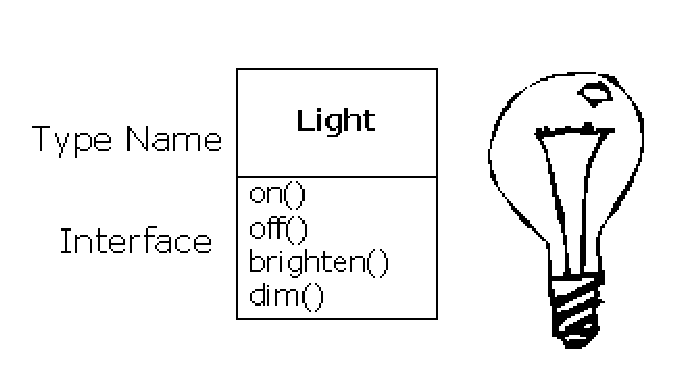
\includegraphics[scale=0.8]{eps/TIJ203.eps}
\end{figure}

\begin{verbatim}
Light lt = new Light();
lt.on();
\end{verbatim}

介面(interface)規範了你能夠對物件發出的請求。不過,
還是得有程式碼來滿足這些請求。這些程式碼加上被隱藏的資料,構成所謂的實作
(implementation)。從程序式設計(procedural programming)的觀點來看,
並沒有太複雜。每個type 都有一些函式對映於任何可能收到的請求。
當你對某個物件發出某個請求,某個函式便被喚起。此一過程通常被扼要地說成:
你送出訊息(發出請求)至某物件,該物件便知道此一訊息的對應目的,
進而執行起對應的程式碼。

本例之中的 type/class 名稱是 Light,特定的 Light 物件名為 lt。你能夠對
Light 物件發出的請求是:將它打開、將它關閉、使它亮些、使它暗些。
本例產生一個Light 物件的方式是:定義lt 這個物件名稱,並呼叫
new 請求產生該種型別的物件。欲發送訊息給物件,可以先標示出物件名稱,
再以句點符號(dot)連接訊息請求。從使用者的觀點出發,
這種「以物件來進行設計」的型式很漂亮。

上圖\marginpar{\fbox{35}}是以所謂 UML(Unified Modeling Language)形式呈現:
每個 class 皆以矩形方格表示,class/type 名稱位於方格上方,你所關心的任何 data
members(資料成員)都置於方格中央,方格下方放置所謂的 member functions
(成員函式),這些函式隸屬於此一物件,能夠接收你所發送的
訊息。通常只有class 名稱及公開的(public)member functions 會被顯示
於UML 圖中,方格中央部份不繪出。如果你只在意class 名稱,那麼甚至
方格下方的部份也沒有必要繪出。
\section{被隱藏的實作細節 \\(The hidden implementation)}
將程式開發人員依各自的專業領域加以區分,對我們的概念釐清大有幫
助。程式開發人員可分為:開發新資料型別的所謂class 創造者,以及在應
用程式中使用他人所開發之classes 的所謂客端程式員
( client programmers)\footnote{關於這個詞彙的使用,我得感謝我的朋友 Scott
Meyers。}。 客端程式員的目標是收集許多可供運用的classes 以利快速開發應用程式。
Class 創造者的目標則是打造classes,並且只曝露客端程式員應該知道的事物,
隱藏其他所有事物。為什麼?因為如果加以隱藏,客端程式員便無法使用,
這意謂class 創造者可以改變隱藏的部份,不必擔心對其他人造成衝擊。
隱藏部份通常代表物件內部脆弱的一環,
它們很容易被不小心或不知情的客端程式員毀壞掉。
因此將實作部份隱藏起來可以減少程式臭蟲。實作隱藏(implementation hiding)
的觀念再怎麼強調也不過份。

在任何相互關係中,存在一個「參與者共同遵守的界限」是一件重要的事情。
當你建立一個class library 時,你會和客端程式員建立起關係。
他可能在某個程式中使用你的library,也可能建立一個更大的library。
如果\marginpar{\fbox{36}}任何人都可以取用某個 class 的所有members,
那麼客端程式員便可以對 class 做任何事情,不受任何管束。
你可能希望客端程式員不要直接操作你的class 中的某些 members,
但如果缺少某種「存取權限控管機制」,就無法杜絕此事,
導致每個物件都赤裸裸地攤在陽光下。

因此,「存取權限控管機制」的第一個存在理由便是,
讓客端程式員無法碰觸他們不該碰觸的事物 - 這些部份應該僅供
data type 內部使用,而非被外界用來解決特定問題。
這對使用者而言其實也是一種服務,因為使用者可以輕易看出哪些事物對他們來說重要,
哪些可以忽略。

「存取權限控管機制」的第二個存在理由是,讓library 設計者得以改變
class 內部運作方式而不擔心影響客端程式。舉例來說,你可能想要簡化開發動作,
改以較簡單的方式來實作某一特定class。但稍後卻發現,
你得重新寫過才能改善其執行速度。如果介面和實作二者能夠切割清楚,
這個工作便輕而易舉。

Java 使用三個關鍵字來設定class 的存取界限:public、private、
protected。這些關鍵字的意義和用法相當直覺。這些被稱為「存取指定詞
(access specifiers)」的關鍵字,決定了誰才有資格使用其下所定義的東西。
接續在 public 之後的所有定義,每個人都可取用。接續在 private 之後的所有定義,
除了型別開發者可以在該型別的 member functions 中加以取用,
沒有其他任何人可以存取。private 就像是你和客端程式員之間的一堵牆,
如果有人企圖存取private members,會得到編譯期錯誤訊息。protected 和
private 很相像,只不過class 繼承者有能力存取 protected members,卻無法存取
private member。稍後還會有對繼承 (inheritance)的簡短介紹。

Java 還有一種所謂的「預設(default)」存取權限。
當你沒有使用上述任何一個指定詞時,用的便是這種存取權限。有時候這被稱為
friendly 存取權限,因為同一個 package 中的其他classes,
有能力存取這種所謂的 friendly members,但在 package 之外,這些 friendly members
形同 private members。

\section{重複運用實作碼 \\(Reusing the implementation)}\marginpar{\fbox{37}}
一旦 class 開發完成並經測試,它應該(理想情形下)代表著一份有用的程式單元
(unit of code)。雖然很多人都對復用性(reusability)有著熱切的期望,但事實證明,
欲達此目的並不容易,你得具備豐富的經驗和深刻的見解。一旦某個 class
具備了這樣的設計,它便可以被重複運用。程式碼的重複運用,
是物件導向程式設計所提供的最了不起的優點之一。

想要重複運用某個class,最簡單的方式莫過於直接使用其所產生的物件。
此外你也可以把某個class 物件置於另一個class 內。我們稱這種形式為
「產生一個成員物件」。新的classes 可由任意數目、任意型別的它種物件組成,
這些物件可以任何組合方式達到你想要的功能。由於這種方式是「以既有的
classes 合成新的class」,所以這種觀念被稱為「複合
(composition)」或「聚合(aggregation)」。複合通常被視為 ``has-a''
(擁有)的關係,就好像我們說「車子擁有引擎」。

\begin{figure}[htbp]
\centering
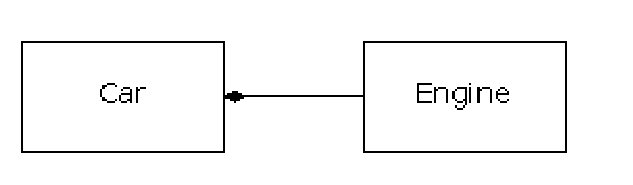
\includegraphics{eps/TIJ204.eps}
\end{figure}

(以上UML 圖以實心菱形指向車子,代表複合關係。我通常採用更簡單的形式,
只畫一條線而不繪出菱形, 來代表聯繫 (association)
關係\footnote{在大多數示意圖中,這樣的表示便已足夠,
通常你不需要在意使用的究竟是聚合或是複合。}。

透過複合,程式員可以取得極大彈性。class 的成員物件通常宣告為
private,使客端程式員無法直接取用它們。
這也使你得以在不干擾現有\marginpar{\fbox{38}}客戶程式碼的情形下,
更動這些成員。你也可以在執行期改變成員物件,
藉以動態改變程式行為。稍後即將探討的「繼承(inheritance)」關係,
由於編譯器會對透過繼承而產生的class 加上諸多編譯期限制,
因此繼承不具備這樣的彈性。

由於繼承在物件導向程式設計中如此重要,使得它常常被高度地、
甚至過度地強調。程式設計新手於是會有一種刻板印象,
以為「應該處處使用繼承」。這會造成誤用,並導致過於複雜的設計。
事實上在建立新class 時, 你應該先考慮複合(composition),
因為它夠簡單又具彈性。如此一來你的設計會更加清晰。有了一些經驗之後,
便更能看透繼承的必要運用時機。
\section{繼承:重複運用介面 \\ Inheritance: reusing the interface}
物件這個觀念, 本身就是十分好用的工具, 讓你得以透過概念
(concepts) 將資料和功能封裝在一起, 因而表述出題域( problem
space)中的想法,不必受迫於使用底層機器語言。這些概念係以關鍵字
class 來表現,成為程式語言中的基本單位。

可惜的是,這樣還是有許多麻煩:建立某個class 之後,即使另一個新的
class 有著相似功能,你還是被迫重頭建立新的class。如果我們能夠站在既有基礎上,
複製class 的內容,然後這邊加加、那邊改改,可就真是太好了。
事實上透過繼承便可達到如此的效果。不過有個例外:當原先的class
(稱為base class 或super class 或parent class)發生變動時,修改過的
「複製品」(稱為derived class 或inherited class 或sub class 或child
class)也會同時反映這些變動。

\marginpar{\fbox{39}}
\begin{figure}[htbp]
\centering
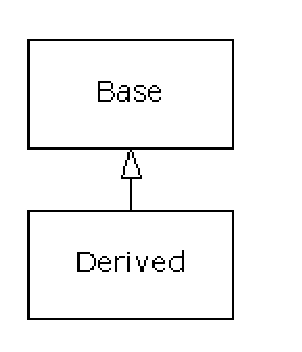
\includegraphics{eps/TIJ205.eps}
\end{figure}

(以上UML 圖中的箭號,是從derived class 指向base class。稍後你便能夠理解,
可以存在一個以上的derived classes。)

type 不僅僅只是用來描述一組物件的制約條件,同時也具備了與其他types
之間的關係。兩個types 可以有共通的特性和行為,但其中某個 type
也許包含較多特性,另一個 type 也許可以處理較多訊息
(或是以不同的方式來處理訊息)。所謂「繼承」便是透過 base types 和
derived types 的觀念,
表達這種介於type 和type 之間的相似性。Base type 內含所有derived
types 共享的特性和行為。你可以使用base type 代表系統中某些物件的核心概念,
再以base type 為基礎,衍生出其他types,
用來表示此一核心部份可被實現的種種不同方式。

以垃圾回收機(trash-recycling machine)為例,它用來整理散落的垃圾。
假設base type 是「垃圾」,那麼每一袋垃圾都有重量、價值等特性,
可被切成絲狀、可被熔化或分解。以此為基礎,
可以衍生出更特殊的垃圾型式,具備額外的特性(例如罐子可以有顏色)或行為
(鋁罐可壓碎、鐵罐具有磁性)。此外,它們的某些行為可能不同
(例如紙張的價值便和其種類與狀態有關)。透過繼承的使用,
你可以建立一個型別階層體系(type hierarchy),表現出你想要解決的問題。

第二個例子是經典的 shape (幾何形狀)範例,
可能用於電腦輔助設計系統或模擬遊戲之中。
Base type 便是 ``shape'',擁有大小、顏色、位置等特性,並且可被繪製、擦拭、
移動、著色。以此為基礎,便可衍生出各種特定的幾何形狀出來:圓形、正方形、
三角形...,每種形狀都可以擁有額外的特性和行為,例如某些形狀可以被翻轉。
某些行為也許並不相同,例如\marginpar{\fbox{40}}面積計算的方式便不盡相同。
型別階層體系(type hierarchy)同時展現了各種形狀之間的相似性和相異性。

\begin{figure}[htbp]
\centering
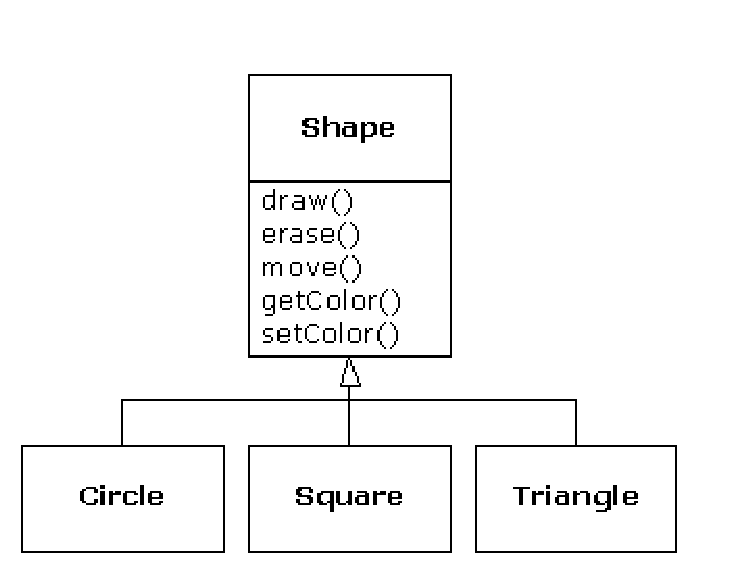
\includegraphics{eps/TIJ206.eps}
\end{figure}

如果我們能以問題原本所用的術語來轉換解答,將會大有益處,
因為你不需要在問題的描述和解答的描述之間,建立起眾多中介模型。
透過物件的使用,type hierarchy(型別階層體系)成了主要模型,
讓你得以直接自真實世界出發,以程式碼來描述整個系統。是的,
對使用物件導向程式設計的人們來說,眾多難以跨越的難關之一便是,
從開始到結束太過於簡單。 對於一顆久經訓練、善於找尋複雜解答的頭腦來說,
往往會在接觸的一開始被這種單純特性給難倒。

當你繼承既有的type 時,便創造了新的type,後者不僅包含前者的所有成員
(但priavte 成員會被隱藏起來,而且無法存取),更重要的是它同時也複製了
base class 的介面。也就是說,所有可以發送給base class 物件的訊息,
也都同樣可以發送給derived class 物件。
由於我們可以透過「可發送之訊息型態」來得知物件的
type,因此前述事實告訴我們,derived class 和
base class 具有相同的type。
例如前一個例子中我們便可以說「圓形是一種幾何形狀」。
透過繼承而發生的型別等價性 (type equivalence),
是了解物件導向程式設計真髓的重要關鍵。

base class\marginpar{\fbox{41}} 和 derived class 有著相同的介面,
而一定有某些實作碼伴隨著此一介面。也就是說,當物件接收到特定訊息時,
還是得有程式碼來執行動作。倘若你只是很簡單地繼承了 class,
然後再沒有做任何事情,那麼 base class 的介面所伴隨的函式,
便會原封不動地被繼承到 derived class 去。這表示 derived class 物件不僅擁有與
base class 物件相同的型別(type), 也擁有相同的行為,這沒什麼趣味。

兩種作法可以產生 derived class 與 base class 之間的差異。第一種作法十分直覺,
只要直接在 derived class 中增加新函式即可。這些新函式並非 base class
介面的一部份。這意謂base class 無法滿足你的需要,因此你得加入更多函式。
這種既簡單又基本的方式,有時候對你的問題而言是一種完美解答。
但是你應該仔細思考,你的 base class 是否也可能需要這些額外功能。
這種發現與更替的過程,會在整個物件導向設計過程中持續發生。

\begin{figure}[htbp]
\centering
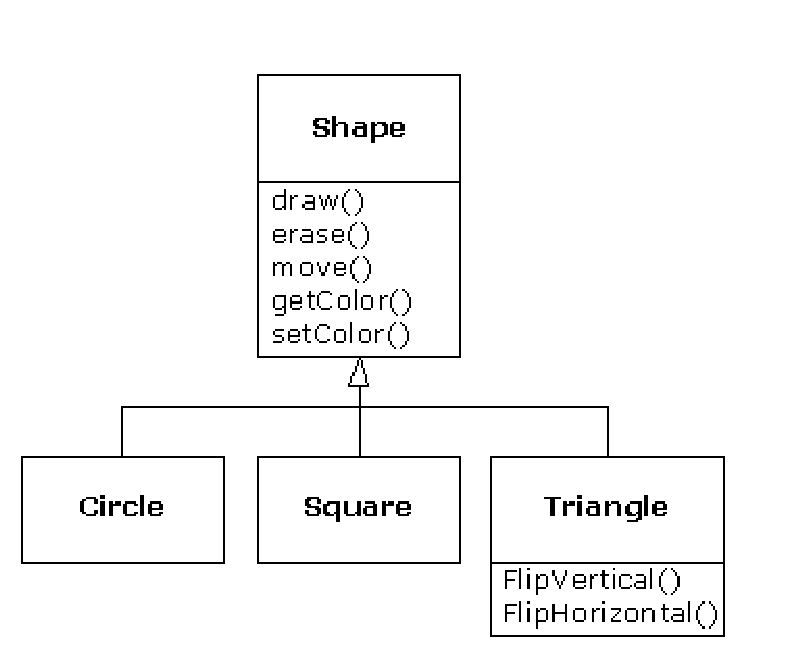
\includegraphics{eps/TIJ207.eps}
\end{figure}

雖然繼承有時候意味著加入新功能至介面中 (尤其 Java 更是以關鍵字
extends 代表繼承),但並非總是如此。
形成差異的第二種方法 (也許\marginpar{\fbox{42}}是更重要的方法)
便是改變既有之base class 的函式行為,這種行為我們通常稱為「覆寫(overriding)」。

\begin{figure}[htbp]
\centering
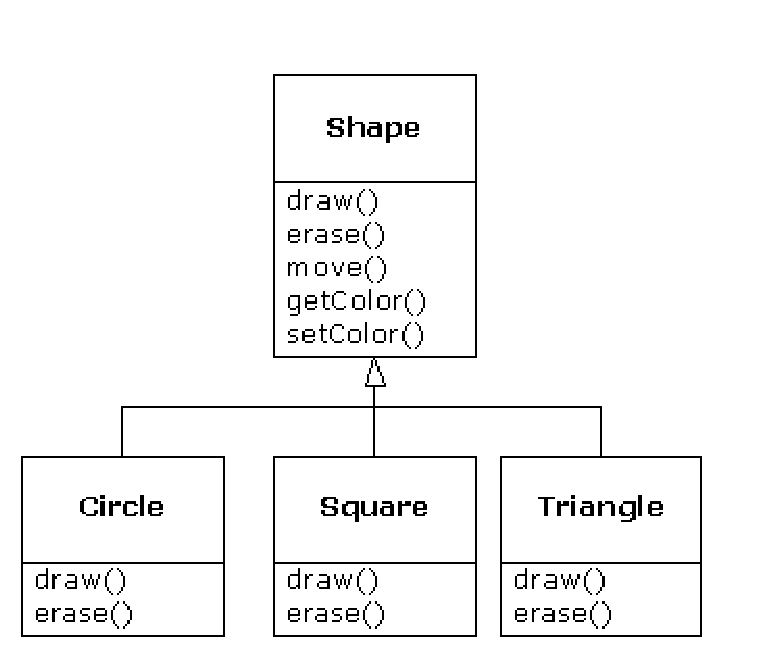
\includegraphics[scale=0.8]{eps/TIJ208.eps}
\end{figure}

想要覆寫某個函式,只須在 derived class 中建立該函式的一份新定義即可。
這個時候你的意思是:「在這裡我使用相同的介面函式,
但我想在新型別中做點不一樣的事情。」

\subsection{是一個(is-a)vs. 像是一個(is-like-a)}
繼承過程中可以進行的動作,仍舊有些爭論。繼承應該「只」覆寫 base
class 的函式(而不加入任何新函式)嗎?如果這樣,便意謂 derived class
和base class 有著完全相同的type,因為它們的介面一模一樣。這樣得到的結果是,
你可以以derived class 物件完全替換base class 物件。這可視為一種「純粹替代
( pure substitution ) 」, 通常稱為「替代法則
(substitution principle)」。就某種意義而言,這是處理繼承的一種理想方式。
我們通常將這種介於base class 和derived class 之間的關係稱為
「is-a(是一種)」關係,因為你可以說「圓形是一種幾何形狀」。
套用繼承關係與否的一個檢驗標準便是,你是否可以有意義地宣稱
classes 之間具備「is-a」的關係。

不過\marginpar{\fbox{43}}有些時候,你還是得將新的介面元素加到derived type 中,
如此也就擴充了介面,進而產生新的 type。新的 type 仍然可以替換 base type,
但這種形式的替換並非完美無瑕,因為 base type 無法取用你加入的新函式。
這種關係我們可以用「is-like-a(像一個)\footnote{這是我發明的詞彙。}」的方式描述。新type 具備和舊
type 相同的介面,但還包含其他函式,所以不能宣稱它們二者完全相同。
以冷氣機為例,假設你的房子裝設了給所有冷卻系統用的控制機制,
也就是說它具備讓你控制冷卻系統的介面。現在,冷氣機壞了,你新裝上一部冷暖氣機。
這個冷暖氣機便「is-like-a(像是一個)」冷氣機,但它可做的事情更多。
但因為房子的控制系統只能控制冷卻功能,所以只能夠和新物件中的冷卻部份溝通。
新物件的介面雖然擴充了,但舊系統除了原介面之外,完全不知道任何其他事情。

\begin{figure}[htbp]
\centering
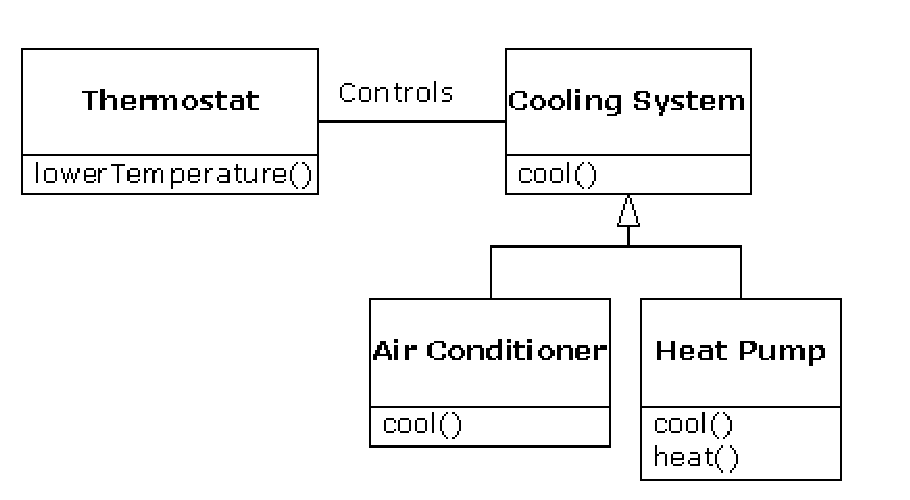
\includegraphics[scale=0.8]{eps/TIJ209.eps}
\end{figure}


當然,看過這樣的設計之後,你便會發現,base class 的「冷卻系統」不夠一般化,
應該改為「溫度控制系統」,使它得以涵蓋加熱功能 - 於是我們便可套用所謂
「替代法則」了。上圖是個範例,說明在設計領域和真實世界中可能發生的事情。

當你了解替代法則\marginpar{\fbox{44}} (substitution principle),
很容易便會以為「純粹替代」是唯一可行之道。事實上如果你的設計能夠依循此種方式,
是滿好的。不過偶而你還是會遭遇到「需要將新函式加入derived class 介面」
的情況。只要仔細檢閱,這兩種情形的使用時機應該是相當明顯的。

\section[隨多型而生的可互換物件]{隨多型而生的可互換物件 \\(Interchangeable objects with polymorphism)}
處理type 階層體系內的物件時,我們往往希望能夠不以它們所屬的特定
type 看待之,而以其base type 視之。如此一來我們所撰寫的程式碼便不會和特定的
type 有依存關係。以幾何形狀為例,用來操作一般化(泛化、
generic)形狀的函式,其實不需要在意其所處理的形狀究竟是圓形、正方形、三角形、
或其他尚未被定義的種種形狀。因為所有形狀都可以被繪製、被擦拭、被移動,
因此這些函式只需發送訊息給「形狀」物件,不需擔心對方怎麼處理這些訊息。

為了擴充物件導向程式的能力,以便處理新狀況,最常用的手法就是加入新
types。此類程式碼的特性就是,不會因為額外加入新型別而受到影響。
例如你可以衍生出幾何形狀的 subtype - 五邊形 (pentagon),
卻不需要修改任何函式 - 只要這些函式僅只處理泛化的(generic)幾何形狀。
這種「透過衍生新的subtype 而擴充程式能力」的手法相當重要,
因為這種能力可以大幅改善設計,使軟體的維護成本降低。

不過,完美的事物並不存在於人間。當我們試著以泛化的base type 來看待
derived type 物件時(例如以幾何形狀來看待圓形、以交通工具來對待腳踏車、
把鸕鶿看做是鳥等等),倘若某個函式要求某一泛化形狀繪製自己,
或是要求某個泛化交通工具前進,或是要求某隻泛化的鳥移動,
編譯器在編譯期便無法精確知道究竟應該執行哪一段程式碼。這是關鍵所在:
訊息被發送時,程式設計者並不想知道哪一段程式碼會被執行;繪圖函式施行於圓形、
正方形、三角形身上完全沒有兩樣,
物件執行時會依據自身的實際型別來決定究竟該執行哪一段程式碼。
如果「知道哪一段程式碼將被執行」對你而言並非必要,那麼當你加入新的子型別
(subtype)時,不需更動函式叫用句,就可以視子型別的不同而執行不同的程式碼。
也因此,編\marginpar{\fbox{45}}譯器無法精確知道究竟哪一程式碼會被執行起來。
那麼編譯器又做些什麼事呢?以下圖為例,BirdController 物件僅處理泛化的
Bird 物件,因此它「對那些Bird 物件實際上是什麼型別」毫不知情。從
BirdController 的角度來看,這麼做是十分方便的,
它將因此而不必撰寫特別的程式碼來判斷所處理的
Bird 物件究竟是什麼型別,也不需要判斷這些Bird 物件會有什麼特別行為。然而,
在忽略Bird 實際型別的情況下,當move() 被呼叫時,物件的實際行為會是什麼?鵝
(Goose)會用跑的還是飛的?還是游泳?企鵝(Penguin)會用跑的還是游水的方式?

\begin{figure}[htbp]
\centering
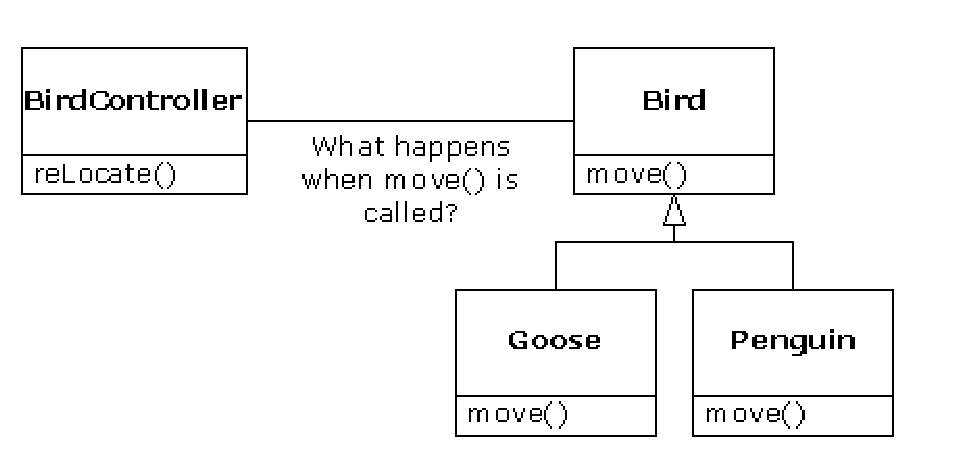
\includegraphics[scale=0.8]{eps/TIJ210.eps}
\end{figure}

這個問題的答案,是物件導向程式設計中最重要的訣竅所在:
編譯器無法以傳統方式來進行函式的叫用。由non-OOP 編譯器所產生的函式叫用,
會以所謂「前期繫結(early binding)」方式來呼叫函式。
這個名詞你過去可能從未聽聞,因為你從未想過能夠以其他方式來辦理。
運用這種方式, 編譯器對叫用動作產生出特定的函式名稱,而聯結器
(linker)再將此叫用動作決議(resolves)為「欲執行之程式碼的絕對位址」。
但是在 OOP 中,程式未到執行期是無法決定程式碼的位址的,
因此當我們將訊息發送給泛化物件 (generic object) 時,必須採用其他解決方案。

為了解決上述問題,物件導向程式語言採用所謂的「後期繫結(late
binding)」觀念。當你發送訊息給物件,
「應被喚起的程式碼」會一直到執行期才決定下來。編譯器還是有責任確定函式的存在,
並對引數 (arguments)、回傳值(return value)進行型別檢驗
(無法對此提供保證者,即所謂「弱型別(weakly typed)」語言),
但編譯器仍舊無法得知究竟會執行哪一段程式碼。

為了達到後期繫結,\marginpar{\fbox{46}} Java
使用一小段特殊程式碼來代替呼叫動作的絕對形式。
這一小段程式碼會透過物件內儲存的資訊來計算函式實體位址
(此一過程將於第七章詳述)。因此每個物件可因為這一小段程式碼的內容不同,
而有不同的行為。當你發送訊息至某個物件,該物件便知道如何反應。

在某些程式語言裡頭(例如C++),你得明確指出是否希望某個函式具備後期繫結的彈性。
這一類語言把所有 member functions 的繫結動作預設為 「非動態」。
這會引起諸多問題,所以Java 將所有member functions 預設為動態繫結
(後期繫結),你不需要加上任何關鍵字,就可以獲得多型 (polymorphism)的威力。

回頭想想「形狀」的例子。整個classes 族系(擁有一致介面的所有 classes)
在本章稍早已有圖示。為了說明多型(polymorphism)特性,我要撰寫一段程式碼,
並在程式碼中忽略型別(types)細節,僅和 base class 溝通。
這樣的程式碼和「型別特定資訊」之間已經解除耦合 (decoupled) 了,
撰寫起來格外簡單又容易理解。舉個例子,當新型別
「六邊形(Hexagon)」透過繼承機制加入classes 族系時,
處理舊型別的程式碼不需任何改變便可以處理新型別。也因此,
我們說這個程式是可擴充的(extensible)。

如果以Java 來撰寫函式(很快你就會學到如何撰寫):
\begin{verbatim}
void doStuff(Shape s) {
s.erase();
// ...
s.draw();
}
\end{verbatim}

上述函式可以和任何 Shape 交談,獨立於它所繪製或擦拭的任何特定物件型別。
如果我們在程式的其他地點用到了doStuff() 函式:
\begin{verbatim}
Circle c = new Circle();
Triangle t = new Triangle();
Line l = new Line();
doStuff(c);
doStuff(t);
doStuff(l);
\end{verbatim}

那麼\marginpar{\fbox{47}}當呼叫doStuff() 時,不論物件之實際型別為何,
都能夠運作無誤。 這是個令人感到驚奇的手法。再看看下面這行程式:
\begin{verbatim}
doStuff(c);
\end{verbatim}

此處當Circle 被傳入這個預期接收Shape 的函式時,究竟會發生什麼事呢?
由於Circle 是一種(is-a)Shape,所以它可被doStuff() 認可。亦即「doStuff()
可發送給Shape」的所有訊息,Circle 都可以接受,所以這麼做是完全安全且合邏輯的。

我們把「將derived class 視為其base class」的過程,稱為「向上轉型
(upcasting)」。cast 這個字的靈感來自於模型鑄造時的塑模動作,up
這個字則是因為繼承階層圖通常將base class 置於上端而將derived class
安排於下端,因此,轉型為一個base type,便是在繼承圖中向上移動,所以說是
upcasting。

\begin{figure}[htbp]
\centering
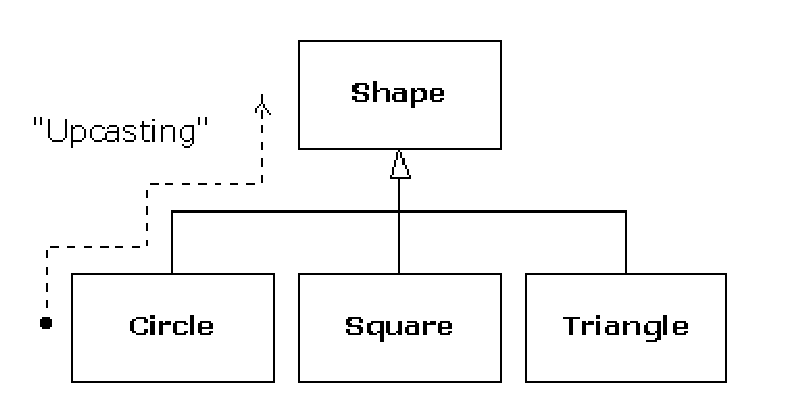
\includegraphics[scale=0.9]{eps/TIJ211.eps}
\end{figure}

物件導向程式一定會在程式某處做些upcasting 動作,
這正是你如何將自己從「執著於實際型別」救贖出來的關鍵。請看doStuff() 內的函式碼:
\begin{verbatim}
s.erase();
// ...
s.draw();
\end{verbatim}
注意,這裡並非表現出「如果你是Circle,請做這些事;如果你是
Square,請做那些事...」。如果撰寫那樣的碼,你得逐一檢查 Shape
物\marginpar{\fbox{48}}件的實際型別,那會帶來極大麻煩,因為每當加入新的
Shape type,你就得改變這段程式碼。這裡所表現的意思是「如果你是Shape,
我知道你自己可以erase(),可以draw(),請妥善進行,並小心細節處不要出錯。」

doStuff() 的內容實在令人感到神奇,不知怎麼地,事情竟然能夠自己搞定。
呼叫 Circle draw() 所執行的程式碼,和呼叫Square 或
Line 的 draw() 所執行的程式碼完全不同。當draw() 這個訊息發往不知所以的
Shape 時,竟會依據該Shape 的實際型別產生正確的行為。這真是神奇,
因為就如先前所說,當Java 編譯器編譯doStuff() 函式碼時,無法精確知道
doStuff() 所處理的型別究竟為何。所以你大概會預期,它呼叫的是
base class 的erase() 和draw(),而不是Circle、Square 或Line
的版本。多型(polymorphism)是整個神奇事件的幕後推手。
編譯器及執行期系統會處理相關細節,你只需知道這件事情會發生,
並知道如何透過它來進行設計,這就夠了。當你發送訊息給物件時,
即便動用了向上轉型 (upcasting),物件仍然會執行正確動作。

\subsection{抽象基礎類別與介面 \\(Abstract base classes and interfaces)}

通常在一個設計案中,你會希望base class 僅僅代表其derived class 的介面。
也就是說,你不會希望任何人產生base class 的實際物件,而只希望他們向上轉型至
base class - 這使得其介面可以派上用場。如果這確實是你的願望,可以使用關鍵字
abstract(抽象的)來標示某種class 是「抽象的」。如果有人試著為抽象類別產生物件,
編譯器會加以阻止。這是強迫某種特殊設計的好工具。

你也可以使用關鍵字 abstract 來描述「目前尚未實作完全」的函式,形成一種戳記
(stub),表示「衍生自此class 的所有型別,都有此一介面函式,
但它目前尚無實作內容」。抽象函式僅能存在於抽象 class 之中。當
class 被繼承,抽象函式必須被實作出來,否則新的 class 仍然是個抽象
class。「建立抽象函式」讓你得以將它置於介面之中,
無需被迫為該函式提供或許毫無意義的程式內容。


關鍵字 interface\marginpar{\fbox{49}}
(介面)又更進一步地發揮抽象概念,阻止任何一個函式被定義出來。
interface 是個常被用到而又十分方便的工具,
因為它提供了「介面和實作分離」的完美境界。此外,如果你想要,
你可以將多個介面組合在一起,不過你無法同時繼承多個一般的或抽象的 classes。
\section{物件的形貌與壽命 \\(Object landscapes and lifetimes)}
技術上來說,OOP 只談論抽象資料型別、繼承、多型等議題。
然而其他議題也可能同樣重要,本節剩餘篇幅涵蓋了這些議題。

一個極為重要的議題便是物件的生成(created)和毀滅(destroyed)。
物件的資料存於何處?它們的壽命如何控制?這裡有一些不同的處理哲學。
C++ 認為效率是最重要的議題,因此將抉擇留給程式設計者。想取得最好的執行速度?
沒問題,請將物件置於stack(這樣的物件又稱為automatic
變量或scoped 變量)或靜態儲存區中,於是程式撰寫時便決定了物件的儲存空間和壽命。
這種安排是把重點擺在儲存空間的配置與釋放的速度上。
某些情況下這樣的安排可能很有價值。不過這麼做卻也犧牲了彈性,
因為你必須在程式撰寫期間明確知道物件的數量、壽命、型別。
如果你企圖解決的是比較一般化的問題(例如電腦輔助設計、倉儲管理、飛航管制系統等),這種方式就過於受限了。

第二種方法是從一塊名為heap(堆積)的記憶體中動態產生物件。在這種方式之下,
除非等到執行期,否則你無法回答需要多少物件、壽命為何、 確切型別為何...等問題。
這些問題只有程式執行時方能給出答案。如果你要求新的物件,只需在必要時候從
heap 產生出來即可。由於執行期對儲存\marginpar{\fbox{50}}空間的管理方式是動態的,
所以從heap 配置空間所耗用的時間,遠大於從
stack 產生儲存空間所需的時間。是的,自stack 產生儲存空間,其動作通
常只是一個簡單的組合語言指令,將stack 指標往下移動;釋放時只要將
它往上移回即可。動態法有一個前提:適用於「物件比較複雜」的情況,
因此不論儲存空間的找尋或釋放時必要的額外負擔,都不致於對物件的產生造成重大衝擊。
動態法帶來的彈性,正是解決一般化程式問題不可或缺的根本。

Java 全然採用第二種方法\footnote{稍後你會看到,基本型別(primitive types)
是特例。}。
每當你想要產生物件,都得使用關鍵字 new 來動態產生物件的實體(instance)。

還有一個議題,就是物件的壽命。在那些「允許物件誕生於stack 內」的程式語言中,
編譯器會判斷物件應該存活多久,並可自動消滅之。但如果在 heap 之中生成物件,
編譯器對其壽命將一無所知。以C++ 為例,你得自行撰寫程式碼來摧毀物件。
因此如果不能正確做好此事,就會引發記憶體洩漏 (memory leaks),這幾乎是
C++ 程式的共通問題。Java 提供了所謂「垃圾回收器(garbage collectioncollector)」
機制,當物件不再被使用,會被自動察覺並消滅。垃圾回收器十分便利,
因為它可以減少你需要考量的因素,也減少你必須撰寫的程式碼數量。更重要的是,
垃圾回收器提供了更高階的保障,避免隱晦的記憶體洩漏問題發生
(這是許多 C++ 專案的痛處)。

本節的其餘篇幅,我們來看看諸多和物件壽命及其景貌相關的其他要素。


\subsection{群集器和迭代器 (Collections and iterators)}\marginpar{\fbox{51}}
如果你不知道你將動用多少個物件,或者不知道這些物件該存活多久,
才能夠解決某個問題,那麼你同樣無法知道該如何儲存這些物件。
如何才能夠知道該為這些物件準備多少空間呢?這其實永遠得不到答案,
因為這些資訊只有在執行期才能獲得。

相對於大多數物件導向設計問題而言,這個問題的解法似乎太過簡單:
產生另一種型別的物件。這個新型物件儲存著一些 reference,代表其他物件。
當然你可以使用array 完成相同的事情,大多數程式語言都提供 array。
不過這裡談的更多。這種新型物件通常被稱為容器(container),
有時也叫群集(collection)。由於Java 標準程式庫以不同的意義使用後一個術語,
本書決定採用「容器」一詞。這個新式物件會適當擴展自己的容量,
以便容納你置入的所有東西。你不需要知道將來會置入多少個物件於容器中,是的,
只要產生容器,它會自行料理細節。

幸運的是,好的 OOP 語言往往都會伴隨一組容器,做為套件的一部份。在 C++ 中,容器是
C++ 標準程式庫的一部份,有時候也稱為 Standard Template Library
(STL, 標準模板程式庫)。Object Pascal 在其視覺化元件庫
(Visual Component Library, VCL) 中亦提供了諸多容器。Smalltalk 提供的容器更完備。
Java 也在其標準程式庫中提供了許多容器。在某些程式庫中,
通用型容器能夠完善符合所有需求,其他程式庫(例如Java)則提供了諸般不同的容器,
符合各類需求。例如vector(向量,Java 稱之為 ArrayList)
為所有元素提供了一致性的存取方式,linked list(串列)
則提供任何位置上的元素安插動作。你應該挑選符合需求的容器。容器還可能包括:
sets(集合)、queues(佇列)、hash tables(雜湊表)、trees (樹狀結構)、stacks
(堆疊)等等。

所有容器都以相同的方式處理元素的置入和取出。通常它們都會提供元素安插函式,
以及元素取回函式。不過元素的取出動作較為複雜,
因為「只能進行單一選取動作」的函式實在是束縛過多,綁手綁腳。
如果你想同時操作或比較「一組」(而非一個)元素時,怎麼辦呢?

迭代器(iterator)\marginpar{\fbox{52}} 為此提供了解決之道。做為一個物件,
迭代器的作用就是用來選擇容器中的元素,並將這些元素呈現給迭代器使用者。身為一個
class,迭代器提供了某種抽象層級,
可將「容器實作細節」和「對容器進行存取動作之程式碼」分離開來。經由迭代器,
容器被抽象化為僅僅是一組序列 (sequence) 。迭代器讓你得以走訪整個序列,
無需煩惱底層結構究竟是 ArrayList 或 LinkedList 或 Stack 或其他。
這種彈性使我們可以輕易更動底層結構而不至於干擾應用程式碼。 Java 在版本 1.0 和
1.1 時代有個名為 Enumeration 的標準迭代器,用於所有容器類別之上。 Java 2
加入更完備的容器類別庫,其中包含名為 Iterator 的迭代器,它能用於老式
Enumeration 力所未逮的許多事情上面。

從設計觀點來看,你需要的其實只是一個可以被操作、用來解決問題的序列。
如果單單某個序列型別就可以滿足你的全部需求,實在沒有理由動用其他類型的序列。
不過,基於兩個理由,你還是得面臨容器的選擇。第一,
不同的容器提供了不同形式的介面和外在行為。stack 具備的介面與行為皆異於
queue,也和set、list 不同。
這些容器之間往往某一種會比另一種更能為你的問題提供彈性解答。第二,
不同的容器在某些操作上有著不同的效率,最佳例子便是 ArrayList 和 LinkedList。
這兩種序列具備完全相同的介面與外在行為,但在某些操作上所耗費的代價,
卻有截然不同的表現。對 ArrayList 進行隨機存取,可以在常數時間 (constant-time)
完成;不論你所選擇的元素為何,所需時間都相同。但是對 LinkedList
而言,「隨機選取某一元素」的動作需得在串列上行進,愈靠近串列尾端,
花費的時間愈久。另一方面,如果你將元素安插至序列中央位置,對 LinkedList
來說花費的代價明顯少於 ArrayList。不同動作的效率高下,
完全取決於序列的底層結構。在設計階段,也許一開始你採用
LinkedList,然後為了調校系統效能,轉而採用ArrayList。迭代器所帶來的抽象化,
使我們在進行諸如此類的轉換時,得以將衝擊降至最低。

最後,\marginpar{\fbox{53}}請你牢記,容器只是個可以將物件放入的儲藏櫃。
如果這個儲藏櫃可以解決你的全部需求,那麼它的實作方式就無關緊要
(對大多數類型的物件而言,這是基本觀念)。如果你所處的開發環境,
有著其他因素所引起的額外負擔,那麼,介於 ArrayList 和 LinkedList
之間的差別可能無關痛癢。你也許只需要一種序列型別。
你甚至可以想像有一個完美的容器抽象化機制,可以根據被運用的方式,
動態改變其底層實作方式。
\subsection{單根繼承體系 (The singly rooted hierarchy)}
OOP 中有個議題,在C++ 面世之後變得格外受人注目:所有classes
最終是否都繼承自單一的base class 呢?Java(以及大多數OOP 程式語言)
的答案是 yes,而且這個終極的 base class 名為 Object。
事實證明,單根繼承體系可以帶來許多好處。

單根繼承體系中的所有物件都有共通介面,所以最終它們都屬於相同的
type。在另一種(C++ 所提供的)設計中,你無法確保所有物件都隸屬同一個基本型別。
從回溯相容的觀點來看,這麼做比較符合C 模型,並且比較不受限制。
但是當你想要進行完全的物件導向程式設計時,就得自行打造自己的繼承體系,
以便提供某種便利性,而這種便利性在其他語言上卻是內建的。
你的程式庫內部可能會有一些不相容介面,你得額外花費力氣將新介面融入你的設計之中
(天啊,面對的可能是多重繼承)。C++ 是否值得為了前述的額外「彈性」這麼做呢?
如果你需要的話 - 也許你在 C 語言上面投資頗多 - 這麼做就有價值。
但如果你剛自起跑線出發,Java 這種方式通常會帶給你更大的生產力。

單根繼承體系(一如Java 所提供)保證所有物件都擁有某些功能。在整個系統裡,
你因此知道可以在每個物件身上執行某些基本操作。單根繼承體系再加上
「在heap 之中產生所有物件」,大大簡化了引數傳遞動作(這也是
C++裡頭十分複雜的問題之一)。

單根繼承體系也使垃圾回收器\marginpar{\fbox{54}} (內建於Java) 的實現更加容易。
所有必備功能都可安置於base class 身上,
然後垃圾回收器便可發送適當訊息給系統中的每個物件。
如果缺乏「單根繼承體系」及「完全透過 reference 來操作物件」的系統特性,
垃圾回收器的實作就會十分困難。

由於所有物件都保證會有執行期型別資訊(run-time type information,
RTTI),所以你必不會因為無法判斷物件的確切型別而陷入動彈不得的僵局。
對於異常處理(exception handling)之類的系統級操作行為而言,這一點格外重要,
並且也能為程式設計帶來更佳彈性。
\subsection[群集類別庫,及其易用性支援]{群集類別庫,及其易用性支援 \\
Collection libraries and support for easy collection use}
容器是一種常常被使用的工具,所以將容器程式庫製成內建形式,是很有意義的事情。
這麼一來你就可以直接使用現成的容器,將它套入你的應用程式中。
Java 提供了這樣的程式庫,而且幾乎可以滿足所有需求。
\subsubsection{向下轉型 vs.模版/泛型 (Downcasting vs. templates/generics)}
為了重複運用容器,我們會以Java 中的某個通用型別(也就是Object)
為對象,進行儲存工作。單根繼承體系意謂「萬物皆為Object」,因此,
如果容器可以裝納 Objects,也就可以儲存任何物件。這使得容器很容易被重複運用。

欲使用這樣的容器,只需將object reference 加入即可,稍後可以將它們取回。
由於容器僅容納 Objects,所以當你將物件的reference 加入容器時,
會向上轉型為 Object,因而遺失自己的精確身份。當你將它取回,你所得到的僅僅是個
Object reference,而非你所置入之物件的確切型別。現在,
該透過怎樣的方式將它變回先前那個具備實用介面的物件呢?

在這裡,轉型動作再度派上用場。但這一次並非是在繼承體系中向上轉型為更通用的型別,
而是向下轉型為更特定的型別。這種轉型動作稱為向下轉型
(downcasting) 。你已經知道, 向上轉型( 例如Circle 轉為\marginpar{\fbox{55}}
Shape)十分安全。但由於你無法得知某個Object 是否為Circle 或
Shape,所以除非你確切知道你所處理的是什麼,否則向下轉型幾乎是不安全的。

不過向下轉型也非全然危險,因為如果向下轉型至錯誤的型別,你會得到所謂「異常
(exception)」的執行期錯誤,稍後我會簡短介紹什麼是異常。但即便有此機制,
從容器中取出object references 時,
你還是需要某種方式來記住這些物件究竟是什麼型別,才能夠放心進行向下轉型。

向下轉型及執行期檢驗動作,都會耗費額外的程式執行時間,以及程式設計者的心力。
何不建立起「知道自己所儲存之物件隸屬何種型別」的容器,
藉以降低向下轉型的需求及可能導致的錯誤呢?解決之道就是所謂的
「參數化型別(parameterized types)」,這是一種由編譯器自動為我們量身訂製的
classes,作用於特定型別之上。舉個例子,如果使用這類參數化容器,
編譯器便可訂製此一容器,使它只能接受(及取出)Shapes。

參數化型別(parameterized types)是C++ 極為重要的組成,部份原因是
C++ 缺乏單根繼承體系。在C++ 中,實現參數化型別的關鍵字是
template。Java 目前並沒有參數化型別,因為單根繼承體系已經可以涵蓋
「參數化型別」的功能。不過目前有一份相關提案,其中採用和C++
template 極為相似的語法(譯註:JSR14,目前已實現於JDK1.4 和
GJ 身上,見www.jjhou.com/javatwo-2002.htm)。
\subsection[管家面臨的兩難:誰該負責清理?]{管家面臨的兩難:誰該負責清理? \\
The housekeeping dilemma: who should clean up?}
每個物件為了生存,都需要動用資源,尤其是記憶體。當物件不再需要記憶體,
就該加以清除,使資源可被釋放、可再被使用。在相對簡單的程式設計環境中,
清理物件似乎不是什麼困難的問題:首先產生物件,然後使用之,
最後它就應該被摧毀。這不難,但你可能遭遇更為複雜的情況。

舉個例子,假設你正在設計機場航空交通管制系統
(同樣的模式在倉儲貨物管理、錄影帶出租系統、寵物寄宿店一樣適用)。
一開始問題似乎很簡\marginpar{\fbox{56}}單:做出一個容器,用來置放飛機,
然後產生新飛機,然後把每一架位於飛航管制區的飛機放到容器之中。
一旦飛機飛離該區域,刪去對應的物件,即是完成了清理動作。

但你或許還有其他系統,記錄著飛機的相關資訊;
或許這些資料目前不會馬上為主控功能所用。
它可能記錄所有即將離開機場之小型飛機的飛行計畫。所以你會有第二個容器,
用來儲存所有小型飛機;每當你產生一個小飛機物件,
同時也把它置於第二容器中。然後,在程式閒置時間(idle time)以一個背景行程
(background process)操作第二容器內的物件。

現在問題更加困難了:何時才是消滅這些物件的適當時機?當你用完某個物件之後,
系統中的某部份還有可能再使用它。此類問題會發生在其他許多情境之中,
在那些「你必須明確刪除物件」的系統中,這件事情顯得格外複雜。

Java 的垃圾回收器被設計用來處理「釋放記憶體時可能會有的種種問題」
(其中並未包含物件清理動作的其他面向問題)。垃圾回收器會「知道」
物件何時不再被使用,然後自動釋放該物件所用的記憶體。這種方式合併了
「單根繼承體系」和「完全從heap 配置記憶體」兩大特性,使得透過
Java 進行程式設計的過程遠較透過C++ 單純。只需做極少量決策,
只有極少的障礙需要克服。

\subsubsection{垃圾回收器vs.效率與彈性 \\
Garbage collectors vs. efficiency and flexibility}
如果這麼做沒有任何瑕疵,為什麼C++ 不率先採行?是的,當然,
你得為程式設計上的便利付出代價,這個代價就是執行期的額外負擔。一如先前所述,在
C++ 中,你可以選擇在stack 上生成物件,它們會被自動清除
(但不具備彈性,無法在執行期依需要而動態產生)。在stack
上生成\marginpar{\fbox{57}}物件,
對儲存空間的配置和釋放來說幾乎是最有效率的方式。在 heap 上生成物件,
代價可就高昂多了。即使完全繼承同一個 base class,完全以多型
(polymorphic)方式來處理函式呼叫,還是需要付出少量代價。
垃圾回收器之所以特別形成癥結,問題在於你永遠不知道垃圾回收動作何時開始、
持續多久。這意謂Java 程式的執行速率會有不一致的現象,因此無法應用於某些情況下,
例如在極重視程式執行速率的場合。此類程式通常稱為即時
(real time)程式 -  雖然並非所有的即時程式設計問題都如此嚴峻。

C++ 的開創者努力爭取 C 程式員的支持,而且成果豐碩,
因此不希望加入任何影響速度的功能,也不期望在那些「程式員可能會選擇
C 的場合」因為 C++ 所引進的新功能轉而採用 C++。這個目標達到了,
但也使得以 C++ 進行設計時需付出「高複雜度」的代價。相對於 C++,
Java 單純許多,但這種單純換來的便是效率上的折損,有時也會失去適用性。然而,
對於解決大多數程式問題而言,Java 是較好的選擇。

\section[異常處理:面對錯誤的發生]{異常處理:面對錯誤的發生 \\
Exception handling: dealing with errors}
自從天地間有了第一個程式語言,錯誤的處理始終都是最困難的問題之一。
因為良好的錯誤處理系統很難設計,所以許多程式語言乾脆直接略去這個議題,
將它留給程式庫設計者,由後者提供「可用於許多情況,但是並非完全徹底」的方法,
或甚至完全忽略這個議題。大多數錯誤處理系統的問題在於,
它們十分依賴程式員自身的警覺性,而非語言本身的法制性。
如果程式員本身不夠警覺 - 通常是因為專案太趕 - 這些系統便容易被忽略。

「異常處理機制」將錯誤處理問題直接內嵌於程式語言中,
有時甚至直接內嵌於作業系統中。所謂異常(exception)是一種物件,
可在錯誤發生點\marginpar{\fbox{58}}被擲出(throw),並在適當的處理程序中被捕捉
(catch),藉以處理特定類型的錯誤。當錯誤發生,
異常處理機制會採取一條截然不同的執行路徑。
也正因為如此,所以它不會干擾程式碼的正常執行。這使得程式碼的撰寫更加單純,
因為你不需要被迫定時檢查錯誤。此外,被擲出的異常、 函式回傳的錯誤值、
函式為表示錯誤發生而設定的旗標值,三者之間有著本質上的差異 -
後二者都可以被有意忽略,異常則無法被忽略,保證一定會在某處被處理。最後一點:
異常為「錯誤情境的確實回復」提供了一種可行方案,是的,不再只能選擇退出
(那是一種逃避),如今你可以校正事情,回復程式的執行,
這種表現是穩健而強固的程式的特質。

Java 的異常處理機制在眾多程式語言中格外引人注目,因為
Java 一開始就將異常處理機制內嵌進來,強迫你使用。
如果你沒有撰寫可適當處理異常的程式碼,便會發生編譯錯誤。
這種一致的態度使得錯誤處理更加容易。

雖然物件導向程式語言常以一個物件表現一個異常(exception),
但異常處理機制並非物件導向的特性。是的,異常處理機制在物件導向語言出現之前,
存在久矣。
\section{多執行緒 ( Multithreading)}
電腦程式設計有一個很基礎的觀念,那就是必須能夠同時處理多個工作
(task)。許多設計上的問題,需得程式停下手頭的工作,處理一些其他事情,
再返回主行程(main process)。辦法很多,早期程式員透過對機器的低階認知,
撰寫中斷服務常式(interrupt service routines),透過硬體中斷的觸發,
暫停主行程的執行。雖然這麼做沒有問題,但這種作法難度較高,也不具可攜性。

有時候,\marginpar{\fbox{59}} 在處理「時間因素極為關鍵」的工作(task)時,
中斷的使用是必要的。但還有其他為數不少的問題,
只需將問題切割為多個可獨立執行的片段,便能夠讓整個程式更具反應力。
這些「可獨立執行的片段」便是所謂的執行緒( threads ) ,
而上述這種觀念便被稱為「多緒」 (multithreading)。
最常見的例子便是使用者介面的運作了,透過執行緒的使用,
雖然還有某些處理動作正在電腦中進行,使用者仍然可以按下按鈕,不受阻礙。

通常,執行緒只是一種用來「配置單一處理器執行時間」的機制。
但如果作業系統支援多處理器的話,不同的執行緒便可以被指派至不同的處理器執行,
真正做到並行(parallel)執行。在程式語言這個層次上提供多執行緒,
所能達到的便利之一便是,讓程式設計者無需考量實際機器上究竟存在多少個處理器。
程式只是邏輯上被劃分為多個執行緒,如果機器擁有多個處理器,不需特別的調整,
程式就能夠執行得快一些。

這使得執行緒聽起頗為單純,但當發生資源共享時,卻會出現隱約的問題。
倘若多個並行的執行緒共用同一份資源,就會引發問題。舉例來說, 兩個行程
(processes)無法同時送出資訊至單一印表機。為了解決這個問題,某些可被共享的資源
(例如印表機),必須在使用時加以鎖定。因此整個過程是:執行緒鎖住某資源、
完成自己的工作、解除鎖定讓其他行程有權力使用該資源。

Java 在程式語言中內建了執行緒功能,讓此一複雜課題變得單純。
由於執行緒功能是在物件層次上提供,因此一個執行緒便以一個物件來表示。
Java 也提供有限的資源鎖定功能,可以鎖定任何物件所用的記憶體
(也算是某種形式的資源鎖定),使得同一時間內只有一個執行緒可使用這個物件。
透過關鍵字synchronized 便可達到此一目的。其他型態的資源就必須靠程式員自行鎖定,
通常的作法是產生一個物件,代表欲鎖定的資源;
所有執行緒在存取這份資源之前都必須先加以檢驗。

\section{永續性 (Persistence)} \marginpar{\fbox{60}}
物件生成之後,只要你還需要它,它就會持續存在。但是一旦程式結束,
它就不再有生存環境了。如果物件可以在程式非執行狀態下依舊存在、依舊保有其資訊,
那麼在許多應用中將大有幫助。因為當程式重新啟動,物件便又能夠復活,
而且仍然具備上次執行時的狀態。當然,你可以簡單地將資料寫到檔案或資料庫,
進而達到這個效果。但是在「萬事萬物皆物件」的精神下,如果能夠將物件宣告為永續的
(persistent),而且由語言系統自動為你處理所有相關細節,不就太好了嗎?

Java 提供所謂的「輕量級永續性(light weight persistence)」,
讓你可以很輕鬆地將物件儲存於磁碟,並於日後取回。稱「輕量級」的原因是,
你還是得自己呼叫儲存、取回動作。除此之外,JavaSpaces(第十五章敘述)
還提供另一種永續儲存功能。未來版本可能還會提供更完整的支援。
\section{Java 與Internet(網際網、互聯網)}
如果Java 不過是程式語言芸芸眾生中的一個,你可能會問,為什麼它如此重要?
為什麼會被宣傳為電腦程式設計革命性的一大步。從傳統程式設計的觀點來看,
答案並不那麼明顯。雖然Java 在解決傳統的個別程式設計問題上非常有用,
但更重要的是,它能夠解決World Wide Web(全球資訊網,萬維網)上的程式設計問題。
\subsection{Web 是什麼?}
Web 一詞,就像其他諸如surfing(網絡衝浪)、presence、home pages
(首頁)等詞彙一樣,乍見之下可能難以理解。對於Internet 這波狂潮,
愈來愈強的反向力量在質問著,這波其勢難擋的變動,經濟價值和結果究竟為何。
如果我們回頭審視其真實面貌,應該會大有幫助。要這麼做,就得先從所謂的「主從
(client/server)」系統開始了解。
這個系統正是電算技術中另一個令人充滿諸多困惑的東西。

\subsubsection{主從式電算技術 (Client/Server computing)} \marginpar{\fbox{61}}
主從式系統的核心概念是,系統中存在一個集中的資訊貯存所,貯存某種形式的資料,
通常位於資料庫中。你想要將這些資訊依據需求,傳佈給某些人或某些機器。
主從概念的關鍵核心便在於,資訊貯存的位置集中於一點。因此每當該點的資訊改變,
變動結果便會傳播至資訊使用者手上。綜合言之,資訊貯存處是一套軟體系統,
能將資訊傳播出去,而資訊和軟體系統所在的機器(可能是單部機器,可能是多部機器)
便稱之為伺服器 (server)。位於遠端機器上、和伺服器溝通以便擷取資訊、處理資訊、
顯示資訊的軟體系統,便稱為用戶端(client)。

主從式計算的基本觀念並不複雜。問題出在你只有單一伺服器,卻必須同時服務多個用戶。
一般而言這會動用所謂的資料庫管理系統,讓設計者得以安排「資料置於表格 (table)
中的佈局方式」,藉以取得最佳使用效果。除此之外,
系統通常也允許用戶增加新的資訊至伺服器。
這意謂你必須確保某個用戶的新資料不會覆蓋另一個用戶的資料,
並確保資料在加入資料庫的過程中不會遺失, 此即所謂的交易處理機制( transaction
processing)。一旦用戶端軟體有所改變,它們必須被設置、被除錯、
然後被安裝於用戶端機器上。整個過程可能超乎你想像的複雜與費力。
如果想同時支援多種不同類型的電腦或作業系統,事情更是格外麻煩。
最後還有一個重要課題:效率。是的,
可能有數以百計的用戶同時向伺服器發出請求,因此即便是一點小小延遲,
都可能帶來重大影響。為了降低延遲,程式員必須努力分散欲處理的工作,
通常是分散至用戶端機器,但有時候會使用所謂的中介軟體 (middleware),
分散至伺服端的其他機器。中介軟體也被用來改善系統的可維護性(maintainability)。

「將資訊分散至多處」的這個單純想法,實作上卻有極多層次的複雜度,
整個問題簡直是棘手得令人絕望。然而主從運算幾乎主宰了半數的程式設計活動。
從訂貨、信用卡交易到各種形式- 股市、科學、政府、個人 -\marginpar{\fbox{62}}
的資料傳佈。過去以來的路線是,每面對一個新問題,就發明一個新的解決方法。
這些方法都很難開發,很難使用,使用者必須一次又一次學習新的介面。
主從架構下的問題需要一個全面性的解決。
\subsubsection{Web 就是一個巨型伺服器 (The Web as a giant server)}
整個Web 體系,實際上就是個巨大的主從系統。更糟的是,
所有的伺服器與用戶端同時共存於同一個網絡中。不過你沒有必要知道這件事,
雖然你可能會為了搜尋想要的伺服器而遍尋全世界,
但同一時間你只要考慮單一伺服器的連接與互動就好了。

剛開始只是很單純的單向過程:向伺服器提出請求,然後伺服器回傳一份檔案,
機器上所執行的瀏覽器(一種用戶端軟體)便根據本機(local machine)
上的格式來解讀這份檔案。但是很快地,人們開始進行更多嘗試,
不單從伺服器擷取檔案,還希望擁有完整的主從架構能力,
讓用戶端也能將資訊回饋至伺服端,例如在伺服器上進行資料庫的搜尋、
將新資訊加入伺服端、下訂單(所需的安全性比早先系統所能提供的還要高)等等。
這樣的歷史變革,是我們可以從Web 的發展過程中觀察到的。

Web 瀏覽器的概念更是向前跨了一大步:同一份資訊可以不需任何改變,
便顯示於各種類型的電腦上。但瀏覽器仍然過於原始,
很快便因為加諸其上的種種需求而陷入困境。是的,瀏覽器缺乏完備的互動能力,
不論你想做什麼事情,幾乎都得面對「將資訊送回伺服器去處理」的問題。
也許花費了幾秒鐘、甚至幾分鐘之後,才發現你所輸入的資料拼字錯誤。
這是因為瀏覽器只是一個觀看資料的工具,無法執行任何即便是最簡單的計算工作。
從另一個角度看,這樣倒也安全,
因為這樣就無法在你的本機上執行任何可能帶有臭蟲或病毒的程式。 

數種不同的方法可以解決這個問題。首先是改善圖形標準規格,
因而得以在瀏覽器中撥放較佳的動畫和視訊。
其餘問題必須透過「在瀏覽器上執行\marginpar{\fbox{63}}程式」的方式加以解決。
此即所謂「用戶端程式開發( client-side programming)」。
\subsection{用戶端程式開發 \\(Client-side programming)}
Web 最初的「伺服器-瀏覽器」設計方式,可提供互動性內容,
但這種互動完全由伺服器提供。伺服器產生靜態的頁面內容,瀏覽器簡單地加以解讀,
然後顯示。基本的HTML 包含有資料收集機制:文字輸入方塊(textentry boxes)、
核取方鈕(check boxes)、選取圓鈕(radio boxes)、列式清單(lists)、下拉式清單
(drop-down lists)等等。此外還包括按鈕 (button):可用於表單 (form)
資料的清除或提交(submit,傳給伺服器)。這種提交動作是透過任何一部
Web 伺服器都會提供的 CGI (Common Gateway Interface,共通閘道介面)
達成。提交內容會告訴 CGI 要做些什麼工作。
最常見的動作便是執行伺服器上某個目錄底下的某個程式,該目錄通常被命名為
``cgi-bin''。 (按下Web 頁面上的按鈕後,如果你觀察瀏覽器上方的位址視窗,
有時候便會看到 ``cgi-bin'' 字樣,後面跟著一大堆冗長不知所云的東西。)
幾乎所有程式語言都可用來撰寫這種類型的程式,Perl 是最常見的選擇,
因為它被設計用來處理文字,而且是解譯式語言,
因此無論伺服器所使用的處理器以及所安裝的作業系統是什麼,Perl 都可以安裝在上面。

今天,許多頗具影響力的Web 站台,完全以CGI 打造。
事實上你幾乎可以用它來達成所有目的。但是以 CGI 程式建構的 Web
站台可能很快會變得過於複雜而難以維護,並衍生「回應時間過長」的問題。
CGI 程式的回應時間和傳送資料量的多寡有關,
也和伺服器的負載以及網絡的擁擠程度有關。而且
CGI 程式的初始化動作先天上就比較慢。Web 初始設計者並沒有預見到,網絡頻寬
(bandwidth)是如此快速地被人們所發展出來的眾多應用程式耗盡。
因此任何形式的動態繪圖動作幾乎都不可能,因為得先產生一個個
GIF 檔案,再一個個從伺服端搬至用戶端。此外你一定也處理過 「驗證表單資料」
之類的簡單事情:你在某個頁面上按下 ``submit'' (提交) 鈕,資料便回送至伺服器,
然後伺服器執行某個 CGI 程式;這個程式\marginpar{\fbox{64}}查覺輸入資料的錯誤,
產生一份HTML 頁面通知你有誤,並將此頁面回傳給你;
於是你回到前一頁面,再試一次。這樣不僅十分緩慢,也不優雅。

這個問題的救星就是用戶端程式開發(client-side programming)。大多數執行
Web 瀏覽器的機器,其實都威力十足,可堪執行龐大的工作。在原始的靜態
HTML 方式下,這些機器只是杵在那兒等著伺服器送來下一個頁面。
「用戶端程式開發」所指的,便是利用Web 瀏覽器來執行某些它能夠執行的工作,
讓網站使用者覺得運行更迅速,操作介面更具互動性。

用戶端程式開發的問題在於,它和一般的程式開發極不相同。參數幾乎相同,
平台卻有差異:Web 瀏覽器就像一個功能受限的作業系統。當然,最後你還是得寫程式,
而且還是得處理那些令人頭暈眼花的問題,並以用戶端程式開發方式來完成解法。
這一節的剩餘部份,我便概觀性地討論用戶端程式開發中的諸般問題和解法。
\subsubsection{Plug-ins}
用戶端程式開發所跨出的一大步,便是發展所謂的 ``plug-in'' 。
透過這種作法,程式員得以下載一小段程式碼來為瀏覽器加入新功能。
那一小段程式碼會將自己安插到瀏覽器的適當位置。它會告訴瀏覽器:從現在開始,
你可以執行這種新功能。於是某些快速、具威力的功能便可透過 plug-in 加到瀏覽器上。
你只需下載 plug-in 一次就好。撰寫 plug-in 並不是件輕鬆的事,
也不是為特定網站而做的事。對用戶端程式開發而言,
plug-in 的價值在於它讓專家級程式員發展新形語言,並將該語言加至瀏覽器中,
而不須經過瀏覽器製造商的許可。因此,plug-in 提供了所謂的後門
(back door),藉以加入新的用戶端程式語言。當然啦,並非所有的用戶端程式語言皆以
plug-in 實作。


\subsubsection{Scripting(描述式、劇本式)語言}\marginpar{\fbox{65}}
Plug-in 帶來了script 語言的蓬勃發展。透過script 語言,
你可以將用戶端程式的原始碼直接內嵌於HTML 頁面中。一旦HTML 頁面被顯示,
負責解譯該語言的plug-in 便會被自動喚起。script 語言先天上比較容易理解,
而且它們只是HTML 頁面內的部份文字, 所以當伺服器收到請求
(request)而欲產生HTML 頁面內容時,可以很快加以載入。犧牲的是你的程式碼的隱密性。
不過通常我們不會使用script 語言做過於複雜的事情,所以隱密性的問題不算太嚴重。

這也點出了script 語言的缺點:只能在Web 瀏覽器中拿來解決特定型態的問題,
更明確地說是指用來建立更豐富、更具互動性的圖形使用介面
(GUIs)。script 語言的確可能解決用戶端程式開發過程中遭遇的百分之八十問題。
如果你的問題恰恰落在這百分之八十之中,script 語言可為你提供簡單快速的開發過程。
在考慮使用諸如Java 或ActiveX 之類更複雜的解法之前,或許你應該先考慮script 語言。

最常被討論的瀏覽器script 語言包括:JavaScript(和Java 毫無關連;
其命名只是為了搭上Java 浪潮而已)、VBScript(程式風貌和Visual Basic 相彷)、Tcl/Tk
(最受歡迎的跨平台GUI 程式設計語言)。還有一些 script 語言不在此列,
有一些正在發展之中。 

JavaScript 或許是其中最被廣泛支援的一種。Netscape Navigator 和微軟的
Internet Explorer(IE)都提供對它的內建支援。此外,比起其他瀏覽器語言,市面上的
JavaScript 書藉或許是最多的。有許多自動化工具可以使用JavaScript 自動產生頁面。
不過如果你已經對 Visual Basic 或 Tcl/Tk 駕輕就熟,
熟練地運用它們應該會比學習另一個新語言更具生產力,
因為你可以將全部心力集中於解決 Web 相關問題。

\subsubsection{Java} \marginpar{\fbox{66}}
如果script 語言可以解決用戶端程式開發問題中的百分之八十,其他的百分之二十
(那些真正很難的東西)該怎麼辦?現今最受歡迎的解決方案便是 Java。
不只因為它是個威力十足的語言,內建了安全功能、跨平台能力、
提供易於進行國際化動作的工具,而且更重要的是,Java
持續擴充其語言功能和其程式庫,得以優雅地處理傳統語言中諸多未能處理好的問題,
像是多緒、資料庫存取、網絡程式開發、分佈式計算。Java 係透過所謂的
applet 來進行用戶端程式開發。

所謂applet 是個小程式,只能執行於Web 瀏覽器上。做為Web 頁面中的一部份,
applet 會被自動下載(就像頁面中的圖形會被自動下載一樣)。
applet 被激化(activated)之後便開始執行,這是它優雅的地方之一 -
當使用者需要用戶端軟體時,便能夠自動將用戶端軟體從伺服器分發出去,
不需事先安裝。使用者絕對可以取得最新版本的用戶端軟體,不會安裝錯誤,
也不需要困難的安裝過程。由於Java 的這種設計,程式員只需發展單一程式,
該程式便能夠自動運作於所有電腦之上 -
只要這些電腦裝有「內建Java 解譯器」的瀏覽器即可(大多數機器都如此)。由於
Java 是個發展完備的語言,所以在將請求送往伺服器之前和之後,
你都可以盡情地在用戶端工作。例如你不必先透過網絡送出請求表單
(form),而後才發現所填的日期或參數錯誤。用戶端的電腦也可以快速繪出資料,
不必等待伺服器完成圖形繪製後才將圖形傳回。
你所獲得的不僅是高速度和高回應能力,也可以降低網絡流量和伺服器負載,
不至於拖累整個Internet 的運作速度。

Java 凌駕於script 語言之上的另一個優點就是,它是編譯式語言,
所以用戶端無法看到原始碼。雖然不需花太多力氣就可以對
Java applet 進行反譯動作,但程式碼的隱藏通常不是什麼重要課題。此外,
還有兩個重要因素。一如稍後所見,編譯過的 Java applet 可以由多個模組構成,
必須引發\marginpar{\fbox{67}}多次對伺服器的存取動作
(hits)才可以下載這些模組。(在Java 1.1 以及更新版本中,透過 Java 保存檔 -
所謂 JAR - 使得所有必要模組都能夠以壓縮形式包裝起來,
因此下載單一檔案便可取得所有模組。)script 程式只需以文字形式整合到
Web 頁面內即可(通常比較小,也減低對伺服器的存取),這對
Web 站台的回應速度很重要。另一個因素是極為重要的「學習曲線」。
不論你過去所學為何,Java 都不是個容易學習的語言。如果你是 Visual Basic 程式員,
那麼投向 VBScript 可能是你的最快解決方案,
它或許可以解決大多數普通的主從式架構問題,這些問題很難拿來印證
Java 的學習。如果你過去對 script 語言已有經驗,那麼付諸
Java 之前,先看看 JavaScript 或VBScript 會對你大有幫助,
因為它們可能更容易符合你的需求,而且使你更具生產力。
\subsubsection{ActiveX}
就某種程度而言,Microsoft ActiveX 和Java 比起來雖然骨子裡是完全不同的技術,
卻足堪與Java 競爭。ActiveX 原先僅用於Windows 系統上,但透過獨立的聯合性組織,
其跨平台能力正在成長。ActiveX 主張,如果你的程式只連接於自身所屬的環境,
那麼此程式便可直接內含於Web 頁面內, 並在支援 ActiveX 的瀏覽器上執行 - IE
直接支援ActiveX,Netscape 則需透過 plug-in 才能辦到。因此 ActiveX
並不侷限於特定的程式語言。舉個例子,如果你曾使用C++、Visual Basic、
Borland Delphi 等語言,在 Windows 平台上進行程式開發,
那麼幾乎不需改變任何程式設計知識,就可以產生 ActiveX 組件
(components)。ActiveX 也讓你得以移轉舊有程式碼至 Web 頁面中。
\subsubsection{安全性Security}
「自動透過Internet 下載程式並執行」聽起來簡直就是病毒作者的夢土。
ActiveX 特別帶起用戶端程式開發中關於安全性的議題。當你點擊某個
Web 頁面,可能會自動下載許多東西:GIF 檔案、script 程式碼、編譯過的
Java 程式碼、ActiveX 組件...。某些東西可能是良性的,例如GIF 檔就不會造成傷害,
script 語言能做的事情通常也都十分有限。Java 的設計理念中,也將
applet 的執行侷限於受到安全保護的砂盒(sandbox)內。
在\marginpar{\fbox{68}}砂盒裡頭,applet 無法對磁碟寫入資料,
也無法存取砂盒外的記憶體內容(譯註:砂盒是西方小孩普遍的玩具,
砂子只能在砂盒裡頭,不能溢出)

ActiveX 剛好位於光譜的另一端。ActiveX 程式開發就和一般的Windows
程式設計一樣,百無禁忌。如果你點擊了某頁面,因而下載了某個ActiveX
組件,此一組件便有可能破壞磁碟中的檔案。這是當然啦,只要你所載入的程式不受限於
Web 瀏覽器,便可以玩出相同的戲碼。來自電子佈告欄系統
(BBSs)的病毒,長久以來一直都是嚴重的問題,Internet 無遠弗屆的速度,
更強化了這個問題。

所謂「數位簽證(digital signatures)」似乎是解答所在。透過數位簽證,
我們可以檢驗程式作者究竟是誰。這個方法著眼於病毒的運作方式 -
病毒作者永遠是匿名的,如果能夠消除匿名行為,那麼每個人都必須為自己的行為負責。
乍看之下不錯,因為這麼做可以讓程式更加實用。
但我懷疑這麼做是否真能消除所有的惡意禍害。而且如果某個程式有臭蟲,
雖非故意造成破壞,仍然會導致問題發生。

透過砂盒(sandbox)的作法,Java 可以避免上述問題發生。存於本機
Web 瀏覽器之中的Java 解譯器(intepreter),在載入applet 的同時便檢驗
applet 是否含有不適宜的指令。因此applet 無法將檔案寫入磁碟,也無法刪除檔案
(而這些正是病毒的生存方式與為害方式)。applet 通常被視為安全,
而「安全」正是可靠的主從系統的支柱。Java 語言中任何可能滋生病毒的缺點,
都會被迅速修正。(瀏覽器軟體會強制施行這些安全限制,
某些瀏覽器甚至允許你選擇不同的安全等級,藉以提供不同等級的系統存取能力。
譯註:不僅瀏覽器可以這麼做,所有Java 程式都可以透過自訂
SecurityManager 的安全策略而辦到。)

你可能會質疑這個方法太過嚴苛,因為這樣就無法將檔案寫入本機磁碟。
舉個例子,你可能會想建立本機資料庫,或是將檔案儲存起來,留待離線時使用。
然而,即便最初的夢想是要讓每個人最終都可以在線上進行所有重要工作,
但大家馬上了解到這可能不切實際(直到有朝一日,
低成本的網絡設備可以滿足大部份使用者的需求)。簽證過的applet 可以回應你的質疑。
「公開金鑰加密」(public-key encryption)可以讓我們檢驗
applet\marginpar{\fbox{69}}是否真的出自它所宣稱的來源。雖然簽證過的
applet 仍然可能毀掉你的磁碟,但你現在可以相信
applet 的作者擔保他們不會進行惡意動作。Java 為數位簽證提供了完整的架構,
所以你還是可以在必要的時候讓applet 踏出砂盒的牢籠。

數位簽證遺漏了一個重要問題,那就是人們在Internet 上的行動速度。
如果你下載某個有問題的程式,而且該程式執行了某些不適宜的動作,
需要多久時間才能發現這個破壞?可能數天,也可能長達數週。到那時候,
如何追蹤究竟是哪個程式造成的破壞呢?而它又究竟在哪個時候幹了些什麼好事?

\subsubsection{Internet vs. intranet}
主從架構的問題,目前最常被採用的解決方案就是Web。所以,
即使只想解決此類問題中的一個子集 -
更明確地說是同一公司內的主從架構上的典型問題 - 一樣可以使用 Web 技術。
如果採取傳統的主從架構解法,你得處理因用戶端電腦平台不同而衍生的種種問題,
也得面臨安裝新的用戶端軟體的種種難處。上述兩種問題都可以透過
Web 瀏覽器和用戶端程式開發來解決。當 Web 技術僅用於特定公司的資訊網絡時,
我們將此網絡稱為 intranet(企業內部網絡)。Intranet 相較於
Internet 能夠提供更高的安全性,因為你可以實際控制對公司內部伺服器的存取動作。
從教育訓練的角度來看,當人們了解瀏覽器的一般概念之後,
便很容易可以處理網頁和 applet 外觀上的差異,進而降低新系統的學習曲線。

安全問題把我們帶到一個用戶端程式開發世界自動形成的角落。
假若你沒有把握你的程式會被執行於Internet 上的什麼平台,那麼你就得格外小心,
別散播含有臭蟲的程式。你需要的是能夠跨平台、具安全性的程式語言,
例如 script 語言或Java。

如果執行環境是 intranet,考量條件就不同了。一個企業內的所有機器都採用
Intel/Windows 平台,是常有的事。在intranet 中你得負責你自個兒的程式碼品質,
並在發現問題之後加以修正。除此之外,
你可能也有以往\marginpar{\fbox{70}}用於傳統主從架構解決方案的程式碼,
每次更新時都得重新安裝用戶端程式。要知道,移轉至
Web 瀏覽器的一個主要原因便是為了減少升級版本的安裝耗費時間。因為,透過瀏覽器,
所有升級動作都被隱藏起來,並自動進行。如果你的應用範圍是在這樣子的
intranet 中,那麼最具意義的解法便是選擇一條「得以使用既有程式碼」的路線,
而不是以一個新語言重新撰寫它們。

如果你覺得很難從這麼多用戶端程式開發策略中進行選擇,
最好的策略便是進行成本效益分析。考量待解問題的諸般限制,再研判何種解法最直接、
最省力。即便採取了用戶端程式開發的路線,你還是得設計程式。
針對自己的應用情境找出最快的發展方式,永遠都是正途。
為那些「程式發展中不可避免必然會碰觸的問題」先做準備,是積極的態度。

\subsection{伺服端程式開發 (Server-side programming)}
截至目前我完全沒有對伺服端程式開發進行探討。當你對伺服器發出請求,
究竟會發生什麼事?大部份時候發出的請求只是簡單如「請傳給我某個檔案」,
你的瀏覽器然後便以某種適當方式來解釋這個檔案的內容:可能是HTML 頁面、圖形影像、
Java applet、script 程式等等。某些更複雜的請求可能希望伺服器進行資料庫交易。
常見的情形便是請求伺服器進行複雜的資料庫搜尋動作,然後由伺服器將結果編排於
HTML 頁面中,再回傳給你。當然,如果用戶端因為Java 或
scrip 語言而更具聰明相,伺服端可以只傳遞原始資料,
然後在用戶端進行頁面編排動作,如此可以加速處理速度,降低伺服器的負載。
另一種情況是,當你加入某個團隊或下了某個訂單,
你可能會想要在資料庫中註冊你的名字,而這得更動資料庫的內容。
如此一來便得透過某些伺服端程式碼,處理這些對資料庫動作的請求,
這便是所謂的「伺服端程式開發(server-side programming)」。過去,
伺服端程式開發通常採用Perl 或CGI,現在則出現了更為複雜的系統。
其中有一種是透過Java-based Web 伺服器,讓你以Java 語言撰寫所謂的
servlets 程式。servlets 及其衍生產物 JSP,
是許多公司在網站系統的\marginpar{\fbox{71}}發展上轉向Java 的主要原因,
尤其是它們可以消除因瀏覽器能力不同而衍生的問題。
(譯註:所謂servlet 一詞是由"server" 和"let" 兩個字合成。
Java 世界常以字尾 ``let'' 表示小東西,例如applet 是由 ``application'' 和 ``let''
合成,表示小型應用程式。servlet 代表小型伺服端程式)


\subsection{另一個截然不同的戰場:應用系統}
儘管Java 骨子裡是個通用性程式語言,有能力解決所有類型的問題(至少理論上如此),但
Java 引起世人的興趣大部份始於applet。正如先前所指出,目前還存在許多有效方法,
可以解決大多數主從架構下的問題。當你離開了applet 戰場
(當然也就從諸多限制中解放了出來,例如從此可以對磁碟寫資料),
便進入了通用性應用系統的世界。在這個世界裡,應用程式都是獨立執行,不須仰賴
Web 瀏覽器之鼻息,和一般程式沒有什麼兩樣。Java 的威力不僅僅來自於它的可攜性,
也來自於它的「可程式化能力 (programmability)」。就在你閱讀此書的同時,
Java 已具備許多功能, 讓你在更短的時間週期內(勝過任何一種語言)開發穩固的程式。

不過,請你了解,魚與熊掌不可得兼,開發速度是以執行速度為代價
(當然也有許多努力正著眼於這一點,尤其是 JDK 1.3 引入了所謂的 hotspot 技術,
能夠大幅改善執行效能)。就像其他語言一樣,Java 具備某些先天上的限制,
使它不適合用來解決某些類型的問題。雖然如此,但Java 的演化成長極為迅速,
每個新版本都讓它在解決更多類型的問題上,具備更高度的吸引力。
\section{分析與設計}

物件導向模式,對程式設計而言是一種全新而截然不同的思考方式。第一次接觸
OOP 專案時,許多人都可能感到困擾。一旦你知道每項事物都被想成是物件,
而且學會了如何以物件導向的思考方式來思考之後,你便有能力利用
OOP 帶來的優勢,開始進行「良好」的設計。

方法(或方法論,methodology),是一組過程和啟發,用來分解程式設計問題的複雜性。
物件導向程式設計誕生之初,已有許多系統化的 OOP 方\marginpar{\fbox{72}}法論存在。
本節便讓你感受一下,採用此類方法來解決問題,是怎樣一種滋味。

「方法論」是充滿實驗性質的一個領域,特別是在OOP 之中。因此,採納某種方法之前,
了解方法本身所欲解決的問題本質,格外重要。對Java 來說更是如此。
Java 係用來降低程式表達上的複雜度(相較於 C 而言)。
這或許可以降低我們對於那些恒常複雜之方法論的需求。在Java 中,
透過簡單方法所能處理的問題模型,比起在程序式語言(procedural languages)
中採用同樣簡單之方法所能處理的問題模型,要大得多。

請注意,「方法論」一詞通常太過偉大,而且承諾過多。其實設計和撰碼時所做的事情,
就是方法。你可能用的是自己發明的方法,而不自知那正是所謂的方法,
但它的確是你所建立、所經歷的一個過程。如果它是個有效的方法,可能只需小幅調整,
就可套用於 Java 身上。不過,如果你不滿意自己的生產力、不滿意程式的執行結果,
你可能會考慮採用正式的方法,或者自眾多正式方法中採擷片段來使用。

一旦你經歷了數個開發流程,最重要的事莫過於:別放棄,做起來其實很簡單。
大多數分析和設計方法,都設定在大型問題的解決方案中。但是請記住,
大多數專案並不落在這個範圍內,
所以你可能是在一個遠比方法論所建議的規模為小的子集中,
成功地分析和設計\footnote{Martin Fowler 所著的
《UML Distilled 2nd edition》(Addison-Wesley, 2000) 之中有極佳例子,
說明如何將一個「有時難以抗拒」的 UML process 降低為一個可管理的子集。} 。
某些類型的程序,不論受到怎樣限制,先經過分析設計往往比直接就開始寫碼高明多了。

這很容易流為一種形式上的固執情結,掉進所謂的「分析導致的癱瘓
(analysis paralysis)」中。你會因為無法在現階段確定每個細節,
而覺得無法往前移動。請記住,不論做了多少分析,還是會有些許系統上的問題,
非得等到設計時期才會顯露;
有更多問題非得等到真正撰寫程式碼或\marginpar{\fbox{73}}甚至程式執行時,
才能夠發覺。正因如此,快速完成分析和設計動作,並實作出測試系統,是相當重要的。

這一點值得特別強調,因為程序式語言(procedural language)帶給我們的歷史因素,
使我們以為,一個團隊在進入設計和實作階段之前,必須周延地考慮任何瑣碎細節,
並善加了解。無疑地,發展DBMS(譯註: Database Management System,資料庫管理系統)
時得徹底了解客戶的需求,但是像 DBMS 這樣的問題正是那種
「形式已定、已被充份了解」的問題。在這樣的程式中,資料庫結構才是重點。
本章所探討的問題類型,卻是我所謂「wild-card」之類的問題。其解法並非單靠
「套用既有解法,換湯不換藥」就可獲得,而是牽扯到一個或多個所謂
「wild-card」因子 - 對於這些因子,目前沒有任何已被充份了解的解法,
因此有研究的必要\footnote{我用來評估此類專案的首要原則是:如果存在一個以上的
wild-card,那麼在建立足堪運作的雛形系統之前,
甚至不要嘗試規畫整個專案會花費多少時間、耗用多少成本。} 。
任何人如果企圖在設計和實作階段前徹底分析「wild-card」問題,都只會落入
「分析導致的癱瘓」下場,因為設計階段缺乏足夠的資料用來解決此類問題。
想要解決此類問題,必須在整個開發週期中不斷來回往返,並採取冒險行為
(這是合理的,因為你所進行的是新事物,而其回報也較高)。
企圖在短期間獲得初步實作,看起來似乎會提高風險,但它反而能夠在
wild-card 專案中降低可能的風險。
因為你會提早發現某個特定方法對問題的解決是否可行。
專案的發展,其實就是風險的管控。

我們常常聽到人家說「建造一個,用完丟掉」。透過OOP,你可能只需丟掉「部份」即可,
這是因為程式碼被封裝為許多classes。第一個階段,你必然會設計出某些有用的
classes,並發展出某些在系統設計上具有價值的想法,而這些
classes 以及這些想法是不需要被丟棄的。因此,在問題的解決上,
快速的第一階段所做的不僅僅只是生產出「對後繼的分析、設計、
實作階段來說十分重要的資訊」,同時也必須建立程式碼的發展根基。

也就是說,如果你正在檢視某個方法論,\marginpar{\fbox{74}}
其中涵蓋十分龐大的細項內容, 並主張使用許多步驟和文件,
那麼想要知道何時才能停止,仍然極其困
難。請記住,你得試著找出以下事物:
\begin{enumerate}
\item 所用的物件是什麼?(如何將案子切割為眾多組成?)
\item 物件的介面是什麼?(你得發送什麼樣的訊息給每個物件?)
\end{enumerate}
確定了物件及其介面之後,就可以開始撰寫程式了。基於某些理由,
你可能還需要更多的描述和文件,但以上兩點是最基本的需求。
整個開發過程可以劃分成五個階段,階段 0 就是對某種結構的運用做最初的確認。

\subsection{階段0:策劃 (Phase 0: Make a plan)}

首先你得決定你的程序(process)將涵蓋那些步驟。聽起來很簡單
(事實上所有動作聽起來都很簡單),但是在開始撰寫程式碼之前,
人們通常不會進行這樣的策劃動作。如果你的計畫是「直接鑽入、開始寫碼」,那也可以
(當你對問題的了解已經十分透徹時,這樣做就很適合)。至少請你同意,這也是一種計畫。

你或許得在這個階段勾勒出某些額外的必要程序結構( process structure),但非全貌。
某些程式員喜歡用所謂的「渡假模式」來工作, 這很可以理解。在這種模式中,
他們不會提出開發過程中的任何結構, 「當它該被完成的時候,它就會被完成」。
這麼做短期間內可能會有吸引力,但我發現,為整個路程訂定一些里程碑,
能夠幫助人們聚集工作的焦點,並在一個個里程碑之間激起對工作的努力,
而不至於只是承擔那「完成專案」的唯一目標。此外,
這樣也能夠將專案切割為許多易於解決的小型目標,並且似乎也比較不會感到艱困
(多一個里程碑,就多了更多的慶祝機會)。

當我著手於故事結構的研究時\marginpar{\fbox{75}}
(我希望有朝一日我能寫本小說),一開始我相當排斥所謂的結構。
我認為只要自然地讓文字流瀉於紙面,就可以寫出最好的作品。但我很快意識到,
當我書寫和電腦相關的事情時,結構對我來說十分清楚,不需特意思考。
但我還是將我的工作結構化了,儘管只在某種半意識狀態。是的,
即便你認為你的計畫很簡單,只不過是直接開始寫碼,
你仍然得以某種方式經歷接下來的幾個階段,詢問並回答幾個問題。
\subsubsection{任務陳述(The mission statement)}

不論你要建立的系統有多複雜,都會有其根本目的;它所處的行業、
它所要滿足的基本需求。如果你觀看的角度可以穿越使用者界面、
與硬體相關或與系統相關的細節、演算法、效率等等,那麼你就可以找出其本質核心所在,
那個單純而直觀的本質。就像好萊塢電影所謂的「中心思想(high concept)」一樣,
你可以用一個或兩個句子加以描述。如此純粹的描述就是一個起點。

「中心思想」極其重要,因為它設定了案子的基調,是任務的陳述。
你不需要一開始就精確捕捉其真髓(因為在此事明朗化之前,
你可能已經處於稍後數個階段中了),但是請持續努力,直到感覺正確為止。
以飛航流量管制系統為例,一開始你可能將「中心思想」鎖定在你所建造的系統本身:
「塔台程式會記錄飛機行蹤」。但是當你將系統縮小到規模極小的機場時,
或許只剩下飛航管制員,或甚至根本沒有人來處理這件事。這裡有一種更實用的模式,
便是不關注欲建立之解法本身,而將重點放在問題的描述:
「飛機抵達、卸客、檢修、讓顧客登機、啟程」。
\subsection{階段1:建立什麼? (Phase 1: What are we making?)}
前一世代的程式設計(所謂程序式設計,procedural design)將此一階段稱為
「產生需求分析和系統規格」。這正是讓人迷途之處;光是那些令人望而生畏的陳述文件,
就足以構成一個大型專案了。這些文件的用意是好的;需求分析所做的是:
「列舉諸般指導方針,使我們知道何時完成工\marginpar{\fbox{76}}作,
以及客戶需求滿足的時間點所在」。系統規格則道出:「為了滿足需求,
程式做了哪些事情(但並不討論如何完成)」。需求分析就是你和客戶之間的契約
(即使該客戶和你服務於同一公司,或甚至它只是某些物件或系統),
系統規格則處於探索問題本身的最頂端,在某種程度上,它是對「問題能否被解決、
需耗費多少時間」兩個問題的探究。由於二者都需要取得人際共識
(而且通常隨著時間改變),所以我認為它們愈少愈好 -
最理想的方式就是採用表列方式和基本圖示,以節省時間。你可能會受到其他束縛,
不得不將它擴展為更大的文件,但是請讓最初的文件保持小而精簡。
只要幾次腦力激盪會議,配合一位有能力動態描述的主持人,就可搞定這樣的文件。
這麼做的目的不僅在於徵求每個人的意見,也是希望促進團隊中協同一致的意見。
或許最重要的是,這可以激起大伙兒對專案的熱情。

在這個階段中,將焦點停駐在欲努力達成的目標核心上,有其必要性:
決定系統應該達成什麼目標。對此,最有價值的工具是所謂的
use cases (使用案例)的聚合。Use cases 會找出系統的關鍵特色,
這些特色可以揭示某些即將動用的根本類別(fundamental classes)。
此類本質性的描述式解答,
可回答如下的問題\footnote{感謝 James H Jarrett 協助。} :

\begin{itemize}
\item 誰將使用本系統?
\item 系統參與者會透過此系統做些什麼事情?
\item 參與者如何透過此系統做到該件事情?
\item 如果其他某人正在做這件事,這件事情會以什麼其他方式運作?
或問「同一參與者是否具有另一個不同目標?」(顯示出變異情形)
\item 透過此系統來進行該件事情時,可能會有哪些問題?(顯示出異常情況)
\end{itemize}

舉例而言,如果你設計的是自動櫃員系統,針對系統功能特定概況而得的use cases,
便能夠描述自動櫃員系統在每種可能情境下的行為。這些情境都被稱為「腳本
(scenario)」,use cases 可被視為腳本的集合體。
你可\marginpar{\fbox{77}}以將某個腳本想像成一個以詢問
「如果...的話,系統會怎麼運作?」為起始的問題。例如「如果某客戶在最近 24
小時內存入一張支票,該支票尚未過戶,帳戶中沒有足夠額度可供提領,
此時自動櫃員系統如何處理?」

use case diagrams(使用案例圖)刻意設計得十分單純,
避免你過早陷於系統實作細節之中:

\begin{figure}[htbp]
\centering
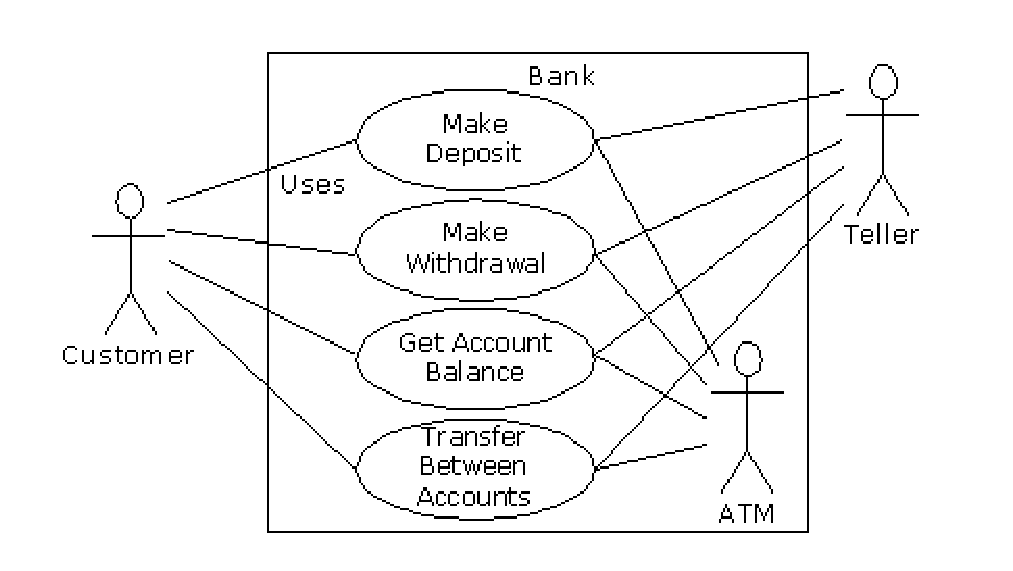
\includegraphics[scale=0.8]{eps/TIJ212.eps}
\end{figure}

上圖的每一個棒狀小人,都代表某個「參與者(actor)」,可以是真人,
也可以是某種形式的代理人(agent)。甚至可能是其他電腦系統,例如本例的
ATM(自動提款機)一樣。方格代表系統的邊界,橢圓代表 use case,
那是系統所能執行的有用工作的描述語句。介於參與者和use cases
之間的直線,代表兩者的互動。

只要系統對使用者而言,長相的確如此,那麼無論系統實際的實作方式為何,
都不會帶來影響。

即使底層系統十分複雜,use case 也沒有必要極度複雜。
其目的只是要顯示使用者所看到的系統的一面。例如:

\marginpar{\fbox{78}}
\begin{figure}[htbp]
\centering
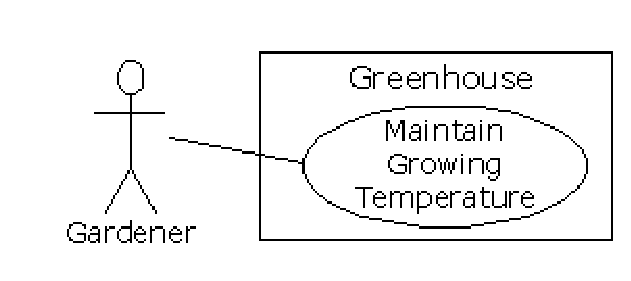
\includegraphics[scale=0.8]{eps/TIJ213.eps}
\end{figure}

use cases 會藉著「找出使用者在系統中可能存在的所有互動情形」而產生需求規格。
試著找出系統中完整的一組use cases,一旦完成,系統功能核心便在你的掌握之中。
專注於use cases 的好處是,它能讓你回歸本質面,
讓你免於陷入那些「無法對工作的達成產生關鍵影響」的因素。也就是說,
如果你擁有了一組完整的use cases,你便有能力描述你的系統,
並有能力進展到下一個階段。或許第一次嘗試時你無法徹底理解,但是不打緊,
所有事物都會即時顯現自己。再說,如果你想要在這個時間點上得到一份完美的系統規格,
最後不免陷入膠著。

如果你真的陷入膠著,可以使用粗略的近似工具,來發動這個階段的工作:
以些許數小段文字來描述系統,同時找尋其中的名詞和動詞。名詞可用以提示參與者、
use case 的環境(context,如上例之大廳)、或是在此 use case 中被操作的人工製品。
動詞可用以提示參與者和use case 之間的互動關係,並指出
use case 中的諸多步驟。你當然也會發現,在設計階段中,
名詞和動詞還可以對應至物件及訊息(但請注意,use case
描述的是子系統之間的互動關係,因此「名詞和動詞」這種技巧僅能做為腦力激盪工具,
無法用來產生use case)\footnote{關於use case,在 Schneider 與 Winters
合著的《Applying Use Cases》(Addison- Wesley 1998)以
及Rosenberg 所著的《Use Case Driven Object Modeling with UML》
 (Addison-Wesley 1999)兩本書中,有更詳盡的解說。} 。

介於use case 和參與者之間的邊界,可以指出使用者介面(UI)的存在,
但不定義任何使用者介面。關於使用者介面的定義及建造過程,請參考
Larry Constantine 和 Lucy Lockwood 合著,1999 年由 Addison-Wesley Longman
出版的《Software for Use》一書,或是親 訪www.ForUse.co網站。

雖然這是一種魔術,\marginpar{\fbox{79}}但是在這個時間點上制定一些基本時程規畫,
還是挺重要的。現在,你已對所要發展的東西有一些概括認識,因此,
對於所需花費的時間,你或許能夠捕捉到一些想法。許多影響因素開始在此處發酵。
如果你估計的時程過長,公司可能決定不開發(如此便能更合理地將資源用於它處 -
這是一件「好事」)。也許某位經理已經評估過此專案所需的時程,並試著影響你的評估。
喔,最好一開始就對時程保持誠實的態度,並儘早處理這個燙手山芋。
許多人嘗試建立精確的時程評估技巧,但或許最好的方法就是仰賴你自己的經驗和直覺。
先憑直覺來估計所需時間,再將它乘以兩倍,最後再加百分之十。你的直覺或許正確,
讓你可以及時完成專案。乘上兩倍是為了把事情做得更像樣,
最後的百分之十則用在潤飾處理上\footnote{對此,我的觀點後來又有所改變。
乘以兩倍再加上百分之十,雖然可以得到合理的估計 (假設不存在太多 wild-card 因子),
但是你仍舊得辛勤工作,才能在時限內完成工作。如果你需要時間以求更精緻的結果,
並在過程中得到樂趣,那麼我相信正確的倍數應該是 3 或4。}。 不論你怎麼解釋,
不論你在呈現如此時程時有著什麼樣的抱怨和運用,最後的結果似乎就是這樣。

\subsection{階段2:如何建立? (Phase 2: How will we build it?)}
在這個階段中,你必須完成設計,其中必須描述classes 的長相、以及 classes
之間的互動方式。「類別 - 責任 - 協同合作關係( Class- Responsibility -
Collaboration,CRC)」卡片在classes 及其互動關係識別上,是個極佳技巧。
這個工具的價值,部份來自於它的技術單純性:只需一組空白的3x5 卡片,寫上一些東西,
便可開張大吉。每張卡片都代表一個class,卡片必須寫上:

\begin{enumerate}
\item class 的名稱。這個名稱很重要,它得反映出class 的行為精髓,令
人望而生義。
\item class \marginpar{\fbox{80}} 的責任(responsibilities),也就是它應做的事情。
通常可以從其成員函式的簡要陳述中獲得
(這些函式名稱應該具備清晰的描述力),但也不排除其他註記。
如果你想要在這個過程中播種以求收穫,那麼,請從一個懶惰的程式員的角度來檢視問題:
「你會期盼怎樣的物件神奇般地出現,一舉解決你的問題?」
\item classes 的「協同合作(collaborations)」關係:哪些classes 會和這個
class 互動?互動(interact)是個意念廣泛的詞彙,它可能是指聚合關係
(aggregation),或只是很簡單地存在某些物件,提供服務給此一
class 的物件。協同合作關係應該考慮到class 的閱聽者。舉個例子,如果你建立起名為
Firecracker(鞭炮)的class, 那麼誰會觀察(observe)它呢?一個Chemist
(化學家)?或是一個Spectator(觀賞者)?前者想知道哪些化學材料可製造鞭炮,
後者能夠說出鞭炮爆炸時的顏色和形狀。
\end{enumerate}


\fbox{%
\begin{minipage}{.93\textwidth}
譯註:CRC card 是Kent Beck 和Ward Cunningham 於1989 年的
OOPSLA ( Object-Oriented Programming Systems, Languages and
Applications ) 學術研討會中, 以一篇《A Laboratory for Teaching
Object-Oriented Thinking》論文提出的。在Timothy Budd 所著的《An
Introduction to Object-Oriented Programming 2nd Edition》(Addison-
Wesley 1997)中有不錯的應用範例。
\end{minipage}%
}
\bigskip

你可能會覺得卡片應該大一點,好讓你可以從中取得你想要的所有資訊。
但它們的小尺寸其實是刻意的,不僅希望讓你的class 保持精巧,
也希望你不要太早鑽進太深的細節中。如果這般小卡片上的資訊無法滿足你的需求,
那就意謂這個class 太過複雜(如果不是因為你考慮得太仔細,就是應該產生更多的
classes 來因應)。理想的class 應該一眼就被了解。CRC card 的出發點,
就是要協助你準備第一份設計方案,以利全貌的取得,同時回過頭來修繕原先的設計。

溝通,是CRC card 帶來的眾多好處之一。最好是不要依賴電腦,在群體中即時完成溝通。
每個人都負責數個 classes (一開始可能沒有 classes 名稱,也沒有其他資訊),
一次解決一個「腳本」,決定哪些訊息會被發送給哪些不同的物件以符合腳本內容,
這樣就彷彿置身於一部生命模擬器中。當你經歷此一過程,你會逐一察覺需要動用哪些
classes、其責任為何、以及它們之間的合作關係。最終你便能填滿卡片中的欄位。
一旦你遍行所有 use cases,一份相當完備的初始設計方案就出爐了。

有一次我和某個開發團隊合作,他們從來沒有以\marginpar{\fbox{81}}
OOP 方式開發過專案。我站在他們面前,在白板上畫出各種物件。
為他們提供設計方案初稿的此次經驗,是我在使用 CRC card 之前,
最為成功的一次諮詢經驗。我們討論著物件應當用什麼方式彼此溝通,然後擦掉某些物件,
以其他物件替代。其實我只不過是把所有 CRC cards 都放在白板上罷了。該團隊
(也就是知道整個專案應該做些什麼事的人) 實際產生了設計內容;
他們真正「擁有」了這份設計。我只不過是藉著詢問適當問題、嘗試建立假設、
接收團隊回饋訊息以修正假設等種種方法,導引整個過程的進行。
整個過程最美好的地方莫過於,該團隊並非透過「對某些抽象範例的探討」
來學習物件導向設計,而是專注於他們最感趣味的設計之上。

當你準備好一組 CRC cards 時,你可能會想要使用UML\footnote{對新手而言,
我推薦先前提過的《UML Distilled, 2nd edition》。}
來為你的設計內容建立更正規的描述。這並非必要,但還是有幫助,
特別是當你想要將圖示投射到牆上,好好沉思一番時。UML 之外的另一個替代方案是
「物件和其介面的文字性描述語句」,甚至可以是「程式碼本身」\footnote{Python
(www.python.org)通常被用來做為「可執行的虛擬碼(pseudocode)」。}
(視程式語言而定)。

UML 也針對系統的動態模型,提供額外的圖示符號。當系統或子系統的狀態移轉行為,
重要到必須以專屬圖示加以表現時(例如在控制系統中), 這些符號就十分有用。
一旦資料成了具支配性的影響因素(例如資料庫),
你可能也需要描述系統和子系統內的資料結構。

當你完成了物件和其介面的描述,你就會知道階段2 的工作已告一段落。
嗯,其實這只是大部份的物件而已,仍然有一些遺漏掉了,得等到階段 3 才有辦法知道。
但這不礙事兒,你只要注意最終是否能夠發掘出所有物件就好了。
雖說若能在整個過程中愈早發掘出來最好,但 OOP 提供了足夠的結構,
因此即使晚一點才發掘出來也不會造成什麼負面影響。事實上在程式發展的過程中,
物件的設計應該發生於五個階段。

\subsubsection{物件(Object)設計的五大階段}
\marginpar{\fbox{82}}
物件的設計並不侷限於程式撰寫時期。事實上物件的設計動作會發生在一連串階段之中。
抱持這樣的看法,對你將大有幫助,因為你不會期盼馬上得到完美的結果,你會意識到,
對物件的行為、外貌長相的理解,是隨著時間而發生的。
這樣的觀點能夠應用於不同類型的程式設計上;某個特定型態的樣式
(pattern)會在一次又一次與問題對抗的過程中浮現出來
(這是《Thinking in Patterns with Java 》一書的主題, 該書可
www.BruceEckel.com 下載)。物件當然也有它們自己的樣式,在了解、
使用、重複運用物件的過程中,便會一一顯現出來。

\begin{enumerate}
\item 物件的發掘。這個階段發生在程式內部分析期間。透過對以下事項的檢視,
包括外在因子和邊界、系統中的元素重複情況、最小概念單元,便可能發掘出物件。
如果你已有一組class libraries,那麼某些物件的存在就很明顯。我們可以透過
classes 之間的共通性來訂定base classes,繼承關係也許此刻就會明朗,
也許還要等到設計後期。
\item 物件的組合:實地發展物件時,你會發現你得增加許多發掘期間未曾出現的新成員。
這些物件的內部需求,可能需要其他 classes 的援助。
\item 系統的建構。這個階段中將出現對物件的更多需求。就像學習過程一樣,
你的物件會逐步演化。由於得和系統中的其他物件溝通和接駁,因此可能得改變對
classes 的需求,甚至加入新的classes。舉例來說,你可能會發現需要動用某些諸如
linked list 之類的輔助性classes,它們包含很少狀態
(state),甚至不含任何狀態,只是用來輔助其他 classes 的運作。
\item 系統的延伸。當你將新功能加入系統,你可能會發現,先前的設計無法輕易擴充。
因此,你或許可以重新建構系統的部份組成,或許是加入新的 classes,或甚至新的
classes hierarchies。
\item 物件的重複運用。\marginpar{\fbox{83}}
對 class 而言,這無疑是最真實的考驗。
如果某人試著將物件重複運用於某個全新情境之中,他也許會找出某些缺點。
每當你更動一個class 以適應更多新程式,那個 class 的一般性原則就會變得更清楚。
最後你終於擁有真正可重複運用的 type - 可以讓大部份物件於特定系統發揮效用。
「可重複運用的types」彼此之間不甚具有共通性,而且,為了被反覆運用,
它們得解決較一般性的問題。 
\end{enumerate}

\subsubsection{物件(Object)發展的指導原則}
上述幾個階段,在你發展 classes 的思路上提供了一些指導原則:

\begin{enumerate}
\item 為特定問題產生一個class,然後讓它在解決其他問題的同時,
漸漸成長茁壯而趨於成熟。
\item 記住,發掘你所需要的classes 和其介面,是系統設計的主要工作。
如果所需的classes 俱已存在,那麼這個專案再簡單不過了。
\item 別強迫自己一開始就要知道所有事情;耐心地一面前進一面學習。
無論如何這都是比較愉快的方式。
\item 開始寫程式;讓某部份先動起來,好讓你可以驗證你的設計,
或是找出設計的盲點。別怕被那些和義大利麵條沒兩樣的程序式
(procedural style)程式碼逼上死路。classes 能夠切割問題,
對於控制無序與混亂很有助益。糟糕的classes 不會拖累優秀的classes。
\item 永保單純。物件若能夠保持小而簡潔,並提供明顯易懂的功能,
絕對比大而無當、介面繁複的對手來得好。每當面臨抉擇,請使用
Occams 的所謂剃刀法 (Razor approach):在眾多選擇中挑出最單純的一個,
因為最單純的classes 永遠是最好的。從小而簡潔出發,
當你更加了解class 的介面特性,便可加以擴充。隨著時間推移,我們很難將元素自
classes 中移除。
\end{enumerate}

\subsection{階段3:打造核心 (Phase 3: Build the core)}
這個階段進行初次轉換,將原始設計轉換為「對於可測試之程式碼的主體部份」
的編譯與執行動作。這麼做能夠驗證架構的正確性,
或找出錯誤所\marginpar{\fbox{84}}在。這當然不會只是一個回合而已,
這是一個開端,後續一系列步驟將能夠來回反覆地建造出系統,一如你在階段 4 中所見。

我們的目標是找出系統架構的核心,這個核心必須完成 - 不論一開始它是多麼地不完整 -
以便產出可運行的系統。你所產生的正是日後賴以為根基的框架
(framework)。你還會進行首次的系統整合與測試,並給予投資者一些訊息,
讓他們知道系統的長相大概是什麼樣子,系統目前的進展又是如何。
理想情況下你還會接觸到某些關鍵性風險。你或許也會察覺出原始架構中可更動、
可改善的地方,這些都是「不做就學不到」的東西。

系統建立過程中,包含對系統進行真實的檢查,也就是依據需求分析和系統規格
(不論以何種形式存在)進行測試。請確認你的測試動作對於需求和
use cases 皆進行了檢驗。系統的核心一旦穩固,也就等於做好了準備,
可以繼續往前進,並加入更多功能。
\subsection{階段4:use cases 的迭代 (Phase 4: Iterate the use cases)}
一旦核心架構能夠運作,你所加入的每一個功能組,本身都可視為一個小型專案。
你會在所謂「迭代(iteration)」過程中將功能組加入。這個迭代過程,
只佔整個發展期相當小的一段時間。

\bigskip
\noindent
\fbox{%
\begin{minipage}{\textwidth}
譯註:迭代 (iteration)是指一種反覆往返的概念。這裡的迭代過程中,
我們發展一個新功能,把它整合到先前系統,加以測試。接著再發展另一個新功能、整合、測試...。如此不斷地反覆往返,系統益形增長。
\end{minipage}
}
\bigskip

一次迭代過程有多大?理想情形下每個迭代過程持續進行一至三週
(隨著程式語言而有不同)。這個過程的最後,你會有一個整合妥當、經過測試的系統,
其功能較先前版本更豐富了。特別有趣的是迭代過程的歸依所在:單一
use case。每個 use case 都是一整套相關功能,
這些功能是你想要在單一迭代過程中加入系統的。這不僅讓你對 use case
的涵蓋範圍有了更好的認識,也讓你得以印證
use cases 的觀念。即使在分析和設計之後,
這個觀念也不應該被丟棄,因為在軟體發展過程中,無論哪一個階段,
它都是最根本的單元。

當你完成你所設定的全部功能\marginpar{\fbox{85}},或是外部期限已到,
而顧客也對現有版本感到滿意,便是上述迭代過程停止的時刻。
(請記住軟體是一種「預訂」
行業。)由於整個過程是反覆往返的,所以你有很多出貨機會,而非只能在單一點上;
如果你的專案採行開放源碼(open-source)策略,在這種反覆往返、
高度倚賴回饋訊息的環境中,能夠如魚得水地獲得成功。

迭代式發展過程,因為許多因素而顯得彌足珍貴。
帶有重大影響的風險可以被提早察覺並加以解決,顧客有足夠機會改變他們的想法,
程式設計者可以獲得更高的成就感,也可以更精準地掌控專案的進行。
除此之外還有個好處,那就是對投資者的訊息回饋,
讓他們可以看到產品中的每一樣事物的當前狀態。這麼做或許可以減少
(甚至完全去除)那些叫人傷透腦筋的狀態回報會議,並能夠堅定投資者的信心,
增加來自投資者的協助。

\subsection{階段5:演化 (Phase 5: Evolution)}
這個階段相當於傳統發展週期中的「維護(maintain)」階段。
其中涵蓋所有零零總總的事情,包括「讓它可以像一開始就被期望的那樣」到
「加一些客戶忘了提到的功能」,甚至更傳統的「修正浮上檯面的臭蟲」和
「隨著需求增加,加入一些新功能」,都算在裡頭。
許多錯誤的認知都被附加於「維護」一詞,使它承擔了品質上的某些欺瞞行為。
部份原因是這個詞彙讓人認為,你的確建立了一個原始程式,
而你需要做的便是為它更換零件、上點機油、並避免生鏽。
或許我們應該選一個更好的詞彙來描述實際上發生的事情。

我選擇以「演化(evolution)」來替代「維護」\footnote{Martin Fowler
的《Refactoring: improving the design of existing code》
(Addison - Wesley 1999)一書(完全以Java 為範例),
至少涵蓋了一個以上的「演化」面向。}。
其意思是,由於無法在第一回合就讓每一件事正確無誤,所以我們需要一些迴旋空間,
一面學習一面回頭修正。隨著你的學習,也隨著對問題本質更加透澈的了解,
需要更正的地方或許不少。如果你能不斷演化,
直到完全正確,那麼你所展\marginpar{\fbox{86}}示的優雅便能取得成功 -
不論是短期或長期。演化,是讓你的程式從
「好」到達「了不起」的關鍵,也是那些「第一回合無法真正了解」
之問題變得清楚的關鍵。它同時也是你的 classes 從「僅適用於單一專案」演化為
「足堪重複運用」的關鍵。

「事事正確無誤」所指的,並非單只是讓程式根據客戶需求和use cases 來運作。
它同時也意謂,程式碼的內部結構對你來說饒富意義,感覺上服服貼貼地組合在一起,
沒有難搞的語法、過大的物件、也沒有任何醜陋的代碼。此外,
一旦程式結構面臨更動(那是生命週期中無法逃避的),要如何生存下去,
你得有自己的看法。如何使這些更動可以做得輕鬆、做得乾淨俐落,更要有自己的判斷。
這不是一朝一夕的功夫。你不僅得了解自己所建的系統,
更得了解程式如何演化(即我所稱的「改變的向度
(vector of change)」)。幸運的是,物件導向程式語言特別擅長支援此類
「持續性修改動作」,是的,由物件所形成的邊界,會主動保持結構免於毀壞。
物件導向 (OO) 程式語言讓你可以進行更動,而你的程式碼不致於處處崩裂
(對程序性程式來說「更動」可能是很嚴重的事)。事實上,提供「演化機制」是
OOP 最為重要的優勢。

有了演化機制,你可以先建立某些看起來近似心中構思的東西,
然後把它拿來和設定需求相比較,看看哪些地方不合要求。然後回過頭去修正、
重新設計、重新實作程式裡頭尚未正確的部份\footnote{這有點像是所謂的
「快速建立原型(rapid prototyping)」。在這種方式下,
你可以用快速但相對不那麼乾淨的方式建立一個原型系統,藉此獲得對此系統的了解。
然後再將原型系統丟棄,好好地重新打造。「快速建立原型」的問題在於,
人們往往捨不得丟棄原型系統, 而想以它為基礎繼續開發。但是你得注意,
由於其中結合了程序式編程方法 (procedural programming)
中「結構不足」的缺點,往往導致混亂,帶來高昂的維護成本。} 。
想出正確解法之前,
你或許得花上好幾次功夫才能解決整個問題,或問題的某一部份。(研究所謂設計樣式
(Design Patterns),對此將有助益。你可以在
《Thinking in Patterns with Java 》書中找到更多參考資料, 此書可自網站
www.BruceEckel.com 下載。)


演化\marginpar{\fbox{87}}也會發生於你正在建立系統的時候。
當你檢查系統是否符合需求,卻發現它並非你想要的東西時,就需要演化了。
當你的系統正在運作,然後你才發現其實你要解決的是另一個截然不同的問題,
這也需要演化。如果你認為這種形式的演化正在發生,那麼你應該歸功於自己,
因為你儘快完成了第一版本,才有辦法判斷它是否的確是你想要的東西。

最該銘記於心的重要事情是,預設情形下,如果你修改了某個class,其 super-classes
和 sub-classes 都應該仍然正常運作。你沒有必要恐懼修改
(尤其是當你已經有了一組測試單元,用來檢驗你所做的修改是否正確時,更無需害怕)。
修改不必然會帶來毀壞,不過,任何修改的結果都應該被限制在 subclasses 和 (或)
你所修改之class 的特定合作者內。
\section{取得成功}
當然,你不會在尚未將規畫仔細繪製下來之前,冒然地動手蓋起房子。
如果你蓋的只是露天平臺,或者只是狗屋,你的規畫也許不會煞費苦心,
但你仍然可能想要稍微描繪個草圖,為自己領路。軟體的發展已經走到了極端。
長久以來,人們並沒有好好地在他們的發展過程中進行結構性規畫,
於是大型專案接二連三地失敗。為了解決這種問題,我們終結了那些瞄準大型專案、
有著令人望而生畏的繁多結構與細節事務的方法論。這些方法論令人畏於使用 -
看起來就像會耗掉你的全部時間於文件撰寫上,使你抽不出時間來寫點程式
(這的確常常發生)。我希望我所指出的是一條中庸之道 - 一把可移動量度的尺。
儘情使用符合你自身需求(以及個性)的方法吧。不論你選擇的方式有多麼簡單,
比起毫無計畫而言,「某種」形式的計畫終究還是可以為你的專案帶來極大的改善。
記住,根據統計,超過百分之五十 (有些評估甚至認為是百分之七十)
的專案以失敗收場。

透過對計畫的遵循 (寧可選擇既簡單又簡短者),並在開始撰碼之前先好好設計結構,
你便會發現,所有的事情,相較於「馬上潛心鑽研、開始亂搞一番」,
是那麼輕易地可以兜在一起,毫不費力。你會得到無上的滿足。我的經驗是,
找出優雅的解決方案,能夠得到極深的愉悅,這種深度愉悅的層次與過去的經驗完全不同;
更像是一種藝術,而不單只是技術。
優雅的方法不只是無聊的消遣,它們總是能夠成功。
它們不但讓你的程式\marginpar{\fbox{88}}更易於建立、易於除錯,
也更易於理解和維護。而這正是經濟價值之所在啊。

\section{Extreme programming(XP)}
從唸研究所開始,我便斷斷續續研讀過不少分析和設計技巧。Extreme
Programming(XP)是我見過最激進、最讓人愉快的一種觀念。在 Kent Beck 所著的
《Extreme Programming Explained》(Addison-Wesley, 2000) 書以及
www.xprogramming.com 網站上,都有對此觀念的闡述。

XP 是程式設計工作上的一種哲學,也是一組實踐準則。
其中某些準則已反映於晚近問世的其他方法論中。XP 最重要、最獨特的貢獻,就我看來,
便是「測試優先(write tests first)」和「搭檔設計(pair programming)」 兩者。
雖然 Beck 強烈主張完整過程,但他也指出,即使只採用上述兩條實作準則,
還是可以大幅提高開發工作的生產力和穩定度。
\subsection{測試優先 (Write tests first)}
傳統上,測試往往被歸為整個專案的最末枝節,在「每件事情都正常運作」之後才被考慮,
其價值只是為了「確認真的沒有問題」。
這種想法使得大家潛意識裡把測試視為一件低優先權的工作。
專門從事測試的人沒有獲得足夠的地位,而且常常被隔離在地下室,
遠離那些所謂「真正的程式研發人員」。測試團隊則回敬說:
『我們就像穿著黑袍,把東西弄壞了就樂不可支。』老實說,
當我找出編譯器的瑕疵時也有相同的感覺。

XP 讓測試工作和程式撰寫平起平坐(甚至有更高的優先權),
這種想法是一種革命性的轉變。事實上你得在撰寫待測程式碼之前,先寫好測試樣例,
而後這些測試樣例便永遠與程式碼同在。每次進行專案整合動作時
(那很頻繁,甚至可能一天兩次),所有測試樣例都必須能夠成功執行。

「測試優先」可以產生兩個極為重要的影響。

首先,這麼做能夠強迫人們把\marginpar{\fbox{89}}
class 的介面定義清楚。當人們試著進行系統設計時,我常常建議他們
「幻想有個能夠解決特定問題的完美 class」做為可用工具。
XP 的測試策略又更向前跨了一步,它明確指出 class
對其使用者而言應該具備怎樣的外貌,同時也明確指出
class 必須有的行為模式。直截了當,毫不含糊。你可以寫下一堆文件、
或是產生所有想要的圖示,來描述 class 應有的行為模式及其外觀長相,
但沒有什麼東西比一組測試來得更為真實。前者像一紙清單,後者卻是一紙契約,
一紙由編譯器與程式共同遵守的契約。
很難有其他東西能夠比一組測試樣例更具體地描述一個 class 了。

產生測試樣例時,你被迫對 class 進行完整而詳細的考量,
並常常因此發現一些需要加入的功能,這些功能也許可能在「以UML 圖、CRC 卡、
use cases 等方式做為思考進行路線」的過程中漏失。

「測試優先」的第二個重大影響是,你得在每次做出一份軟體成品時,
都將所有的測試樣例執行一遍。這麼做可以涵蓋整個測試環節的另一半,
也就是編譯器所主宰的部份。如果你從這個角度來看程式語言的發展,你會看到,
技術面上最實際的改善其實是以測試為中心:組合語言只檢查語法正確與否,
C 卻加進了某些對語義的限制,避免型別(types)被誤用。
OOP 語言加進的語義限制更多 - 如果你把這些限制視為某種形式的測試的話。
「資料型別是否被妥善運用」和「函式是否被正確呼叫」
都是由編譯器和執行期系統所進行的測試。
我們已經看到了這些測試內建於程式語言後的結果:人們能夠撰寫更複雜的系統,
並讓它們運作無誤,但所花費的時間和力氣卻更少了。我曾對此苦思許久,
現在我意識到,上述動作都是測試:你有可能弄錯一些東西,
而內建測試功能的安全網會告訴你,有問題發生,並指出問題所在。

但是「自程式語言本身的設計切入,藉以提供內建測試機能」,所能做的也就這麼多了。
某些情形下你得適時介入,補足完整測試的缺口,藉以對你的程式進行整體檢驗。
難道你不希望像編譯器不時從旁照料一般地,
讓\marginpar{\fbox{90}}這些測試樣例一開始就能夠適時派上用場嗎?
這也就是你之所以必須「先寫下測試樣例,並在每次做出一份軟體成品後便自動執行測試」
的原因。 如此一來,你的測試樣例便能成為程式語言所提供之安全網的延伸。

使用那些愈來愈具威力的程式語言時,我發現一件事情:
由於我知道這些語言有能力使我不必耗費時間於程式臭蟲的捕捉,
所以我愈來愈敢嘗試一些尖銳的實驗。 XP 的測試體系對整個專案來說,所做之事亦同。
因為你知道你的測試樣例,絕對有能力捕捉到你所引入的所有問題,
所以你可以在任何必要的時候,進行大幅度修改,不必憂心整個專案陷入混亂狀態。
這真是太有威力了。
\subsection{搭檔設計 (Pair programming)}
我們向來被諄諄教誨,嚴守個人主義。在學校裡頭,成敗都操之在己。與左右鄰居合作,
就被視為「作弊取巧」。媒體,尤其好萊塢電影,也告訴我們,
英雄總是反抗無知的服從\footnote{雖然有點大美國主義,
但是好萊塢的故事的確流傳各地。} 。搭檔設計 (pair programming)
悖離這種強烈的個人主義。程式員常常被視為個體存在的典範- 就像 Larry Constantine 
喜歡說的「牛仔撰碼員(cowboy coders)」。XP 背棄這種想法,
認為應該兩個人合用一部工作站合夥寫程式才對。而且寫程式的環境應該是
「在一大塊空間裡頭擺一堆工作站」,不應該在其中樹立室內設計師最喜歡的隔板。
事實上,Beck 說,如果想皈依 XP,第一件事情應該是拿起螺絲起子、L 形鈑手,
把所有造成阻礙的東西通通拆\footnote{包括 (特別是) 擴音裝置。
我曾經在某家公司任職,這家公司強烈要求,打給所有業務主管的每一通電話,
都必須加以廣播。這麼做時常打斷我們的工作。管理者無法想像,
擴音裝置這麼「重要」的服務,有多麼讓人受不了。趁著四下無人,
我最後剪掉了擴音機的電線。} 。(那麼當然就得有個經理級的人物,
有能力移轉來自設備部門的忿怒囉)

搭檔設計(pair programming)\marginpar{\fbox{91}}
的價值在於,當某個人思考,另一個人就實際撰碼。
從事思考的那個人得將整體宏觀牢記於心 - 不僅僅是對手邊的問題徹底了解,
同時還得熟記 XP 的諸般實踐準則。舉例來說,兩個人一起工作,
就不太可能會有一個人跳出來說:「我可不想先寫測試樣例。」
如果一人陷入困境,兩個人就可以交換角色。如果兩人都陷入困境,
那麼他們兩人發呆的樣子,可能會被整個工作區中的某個可以幫得上忙的人發現。
這樣子搭檔工作,可以讓事情更平順,並依計畫前進。不過,或許更重要的是,
這樣子能讓程式設計變得更與人互動,更充滿樂趣。

我已經在我的某些研討會的習題中加入搭檔設計理念,而我發現,
這似乎相當程度地改善了每一個人的經驗。
\section{Java 為什麼成功}
Java 能夠取得如此的成功,原因在於其目標的設定:
為當今開發人員解決他們所面臨的諸多問題。提高生產力是 Java 的終極目的。
生產力來自於許多層面,但是 Java 語言希望從語言層面提供儘可能的協助。
Java 的目的在實用;Java 語言的根本考量,就是為程式員爭取最多的利益。
\subsection[易於表達、易於理解的系統]{易於表達、易於理解的系統\\
Systems are easier to express and understand}
被設計用來「與待解問題相稱」的class,先天上就有較佳的表述能力。
這意謂當你撰寫程式碼時,並不使用電腦術語 - 亦即解域 (solution space)
空間中的術語,而是以題域空間(problem space)中的術語來描述解法。
如此一來便能夠以高階觀念來處理問題,而且每一行程式碼可以做的事情就更多了。

易於表達所帶來另一好處便是維護,
而維護佔了整個程式生命週期中極大的成本比例
(如果那些數據報告可信的話)。如果程式易於理解,便相對地易於維護。
這也同時可以降低文件撰寫與維護的成本。

\subsection{透過程式庫(libraries)發揮最大槓桿效應}\marginpar{\fbox{92}}

開發程式的最快途徑,就是使用現成的東西:程式庫(library)。Java 的主要目標之一,
便是讓程式庫的使用更容易。「將程式庫轉換為新的 data types (classes)便是
Java 達成此一目標的手段。因此,引入程式庫,意謂將新的 types 加到程式語言裡頭。
由於Java 編譯器會留意程式庫被使用的方式 -
保證初始化動作和清除動作確實正確地執行,並確保呼叫函式的方式合乎規矩 -
你可以專注於程式庫的運用,而不必擔心如何製造它們。

\subsection{錯誤處理}
「錯誤處理」在 C 裡頭向來是個聲名狼藉的問題,而且常被忽略 -
只能祈求上天給你好運。如果你所開發的程式很大,很複雜,
那麼大概沒有什麼事比得上「程式某處暗藏一個錯誤,
我們卻對其發生原因毫無頭緒」還要糟糕吧。 Java 的異常處理
(exception handling) 便是「一旦發生錯誤,保證一定通知你,
並讓你採取一些處理動作」的機制。
\subsection{大型程式設計}
對於程式的大小和複雜度,許多傳統語言都存在若干內建限制。以 BASIC 為例,
它對一般等級的問題,有著最棒的快速解決方案。但是當程式的長度超過數頁,
或是逾越該語言的標準題域之外,你就會像「在一池黏稠液體中游泳」一樣,動彈不得。
你所使用的程式語言何時會失去作用?噢, 沒有一條明白的界線。即使存在界線,
你還是會忽略它。因為你總不能說:「我的 BASIC 程式現在太大了,我得重新用
C 寫過!」所以你會試著硬塞幾行進去,藉以增加新功能。
就這樣不知不覺付出了額外的成本。

Java 具備大型程式設計能力- 也就是抹除了小程式和大程式之間的複雜度界線。
如果你只是想寫一個 "Hello World" 小程式,當然不需動用 OOP,
但是當你需要用到時,這些功能唾手可得。而且編譯器會積極找出臭蟲所在,
不論對小程式或大程式,一律如此。

\marginpar{\fbox{93}}
\section{過渡策略 (Strategies for transition)}
如果你大量採用 OOP,那麼你的下一個問題可能是:「我要如何才能夠讓我的上司、
同事、部門、同儕們都開始使用物件呢?」想想你,一個獨立的程式員,
如何開始學習一個全新的程式語言和一個全新的設計思維?其實你辦到了。
首先是訓練和範例教學,然後是試驗性的專案,讓你感受一些基本原理,
而不需要做一些頭昏眼花的事情。接下來就是一個「真實世界」中的專案,
這個專案真的能夠做一些有用的事情。在此專案過程中,
你不斷閱讀、向高手請教、和朋友交換心得,藉以持續進行學習。
這就是有經驗的程式員轉換到 Java 跑道時可以採取的方式。當然,想要轉換整個公司,
必然會造成一定程度的群體變動,但是請記住,個人所採取的方式,
仍舊可以在每一個步驟中派上用場。
\subsection{實踐準則}
想要過渡到 OOP 和 Java,可以參考以下建議的實踐準則:
\begin{enumerate}
\item 訓練
\

第一步便是某種形式的教育。別忘了公司在程式碼上的投資,
並且努力不要讓任何事情處於混亂狀態超過六到九個月 -
雖然每個人都對介面運作的方式感到困惑。挑選一小群人來進行教育,
這一小群人最好是個性好奇、 能夠彼此合作、能夠在學習
Java 的時候彼此奧援的人。

有時候我也會建議另一種作法,一次教育公司裡的所有階層,
包括對決策高層的概觀性說明,以及對專案開發者的設計和撰碼課程。
這種方式特別適合小型公司進行根本性的移轉,或是對大型公司的部門層次來進行。
不過,由於這會帶來較高的成本,所以也有人選擇從專案層次的訓練開始,
先做個前導性專案(可能邀請外聘講師),再讓專案中的成員變成公司其他成員的老師。

\item 低風險專案\marginpar{\fbox{94}}
\

先以低風險專案做為試探,並允許錯誤發生。獲得些許經驗之後,
便可以將這個前導團隊的成員播種到其他專案去,或把他們視為 OOP 技術支援幕僚。
第一個專案可能無法一蹴而成,所以不應該挑選會對公司產生重大影響的案子。
這個專案應該簡單、能自我控制、具啟發性 - 意謂這個專案應該產生某些
classes,對公司其他人開始學習Java 時帶來一些意義。
\item 向成功借鏡
\

起跑之前,先找一些有著良好物件導向設計的範例出來閱讀。通常,有相當的機會,
別人早已解決了你的問題。就算沒有人恰巧解決你的問題,你也有可能應用所學,
修改他人設計的抽象方法,套用在自己的需求上。這也就是設計樣式
(design patterns)的一般概念。《Thinking in Patterns with Java》
一書涵蓋這個主題,你可以自 www.BruceEckel.com 下載。
\item 使用既有的程式庫 (libraries)
\

更換跑道至 OOP,經濟上的主要動機便是能夠以 class libraries 的形式,
輕鬆地重複運用既有的程式碼(本書廣泛使用的 Java 標準程式庫更是如此)。
當你能夠把既有的程式庫當做基礎,建立物件並加運用,便能產生最短的程式開發週期。
不過某些程式設計新手可能無法意識到這一點,也可能沒有發現到程式庫的存在,
抑或過度迷戀程式語言的魅力,總想自己動手寫一些早已存在的 classes。
如果你能夠早點在這個過渡過程中努力找出他人所寫的程式碼,並加以重複運用,
就能夠透過 OOP 和 Java,取得最大的成功。
\item 不要以 Java 重寫既有的程式
\

將那些既有的、函式風格的程式碼,重新以 Java 寫過,
對時間而言通常不是最佳運用方式。如果你一定得把它們轉向物件形式,你可以運用
Java 原生介面 (Java Native Interface),用以和 C 或 C++ 程式接軌。
本書附錄 B 對此介面有所討論。這麼做可以得到漸進的好處,
特別是當那些程式碼被選定重複運用時。不過這麼一來,
可能你就無法在剛開始的幾個專案中\marginpar{\fbox{95}}看到驚人的生產力提升 -
這一點唯有在全新專案中才有可能出現。Java 和 OOP 的出眾,
最能夠表現在讓一個專案的概念成真、落實。
\end{enumerate}

\subsection{管理上的障礙}
如果你是一個管理者,你的工作便是為你的團隊爭取資源、
排除所有影響團隊成功的障礙,並試著提供最能帶來生產力、
最讓人樂在其中的工作環境,讓你的團隊成為最有可能展現奇蹟的團隊,
達成那些不可能的任務。 遷移至 Java 平台所需付出的成本,
會落在以下所列的三個範疇內。如果這並不會讓你付出什麼代價,那真是太好了。有些
OOP 替代方案,是專門為 C 程式員 (或其他程序式語言的使用者)
所組成的團隊量身提供的。雖然,相較於那些替代方案,遷移至 Java
平台所需付出的代價,顯然低廉多了,但不論再怎麼低廉的成本,依舊不能不花任何成本。
此外,在嘗試將 Java 推廣到你的公司之前、在著手進行遷移計畫之前,
你得先知道路上可能有的一些絆腳石,才好應付。
\subsubsection{起動成本}
遷移至 Java 平台,所需的成本,不單只是取得Java 編譯器而已
(Sun Java 編譯器是免費的,所以這談不上是顆絆腳石)。如果你願意投資在訓練上面
(可能得請專家為你的第一個專案提供顧問諮詢),
並且找到了可解決你的問題的程式庫並加以購買,
而不是試著自己重新開發這些程式庫,那麼你的中長期成本會降至最低。
這些都是得花費實際金錢的成本, 必須納入專案提案書。此外,可能有一些隱藏成本,
來自於「新語言的學習」和「可能導入的新設計環境」所引起的生產力損耗。
訓練和顧問諮詢無疑能夠將這些成本降到最低,
但是團隊成員也必須克服他們自身在了解新技術時湧現的掙扎。在這個過程中,
他們會犯下更多錯誤 (這也是一種特色,因為大家都公認錯誤是通往學習的捷徑) ,
而且生產力降低。儘管如此,面對某些類型的問題,即便大家還只在學習
Java 的過程中,還是有可能比「停留於 C 的使用」帶來更好的生產力 (雖然,
所犯的錯誤或許更多,每天所完成的程式碼或許更少)。
\subsubsection{效能問題}\marginpar{\fbox{96}}
一個常被問到的問題是:「OOP 不會將我的程式變得既肥且慢嗎?」這個問題的答案是:
「視情況而定。」 Java 所提供的額外安全功能,傳統上是犧牲諸如 C++
語言所具備的效能而來的。諸如 ``hotspot'' 之類的技術和編譯器的技術,
多數都能夠大幅提高執行速度;此外還有更多致力於效能提升的努力,正在持續進行。

如果你關注的事情集中在「快速建立原型」上面,你可以匆匆將所有組成拼湊起來,
略去效能上的考量。如果你使用的是其他廠商提供的程式庫,
它們通常都已經由供應商最佳化了,因此在快速開發模式下,效能通常不是問題所在。
當你已經擁有一個想要的系統,如果它夠小而且夠快,你的工作就算告一段落。
如果不是這樣,你就得開始使用一些效能研判工具
(profiling tool)來進行調整,看看能否改寫小部份程式以提高速度。如果不行,
就得找找看有沒有什麼修正手法可以施行於底層,使上層程式碼不需要隨之更動。
一旦這些方法都束手無策,你才需要更改設計。由於效能在設計中佔了極重要的地位,
所以效能必須成為設計良窳的評量依據之一。藉由快速開發方式,
提前找出效能的癥結所在,可以帶來好處。

如果你發現某個函式正是效能瓶頸所在,你可以 C/C++ 重寫那個函式,
並以 Java 原生函式 (native methods)與之接軌,這個主題見本書附錄 B。
\subsubsection{常見的設計錯誤}
一旦你的開發團隊採用 OOP 和 Java,程式員通常會經歷一連串常見的設計錯誤。
通常是因為早期專案的設計和實作上沒有從專家那兒取得足夠的回饋訊息。
這可能是因為沒有在公司內培養出專家,也可能是因為存在著對固定顧問諮詢的反對聲浪。
很容易就可以感受到你是否在整個週期中過早了解 OOP,並走偏了方向。有些事情,
對熟悉此語言的人來說平淡無奇,對新手而言卻是十分重大的討論議題。
藉由經驗豐富的外聘專家提供訓練與顧問諮詢,可以避免許多傷害。

\section{Java vs. C++?}\marginpar{\fbox{97}}
Java 看起來很像C++,而且如此成熟,似乎應該有足夠的份量取而代之。
不過我開始質問這種思考邏輯。畢竟 C++ 仍然具備了某些 Java 沒有的特色,
而且雖然有許多承諾顯示 Java 終有一天會和 C++ 一樣快,甚至更快,
甚至我們也看到了一些效能上的持續進展,但是並沒有什麼驚人突破。再者,
整個程式開發環境仍然對 C++ 有持續性的關注,所以我不認為 C++
會在任何可見的近期內消失。 (程式語言似乎永遠隱而不退。在我的某次
Java 中/高階研討會上,Allen Holub 宣稱,目前最被廣泛使用的兩個語言分別是
Rexx 和 COBOL。)

我於是開始思考 Java 的長處,其戰場其實和 C++ 稍有不同。C++
這個語言並不試著為某種類型的問題量身打造。一般而言它可融入許多不同的方法,
解決種種問題。有些 C++ 工具將程式庫、組件模型
(component models)、程式碼產生工具 (code-generation tools) 結合在一起,
藉以解決視窗環境下 (例如 Microsoft Windows) 及終端用戶相關的應用程式發展問題。
但是,Windows 開發市場中最被廣泛使用的工具是什麼? 是
Microsoft Visual Basic(VB) - 儘管 VB 所產生的程式碼類型,
會在程式長度超過數頁之後就變得難以管理
(而且其語法肯定讓人感到困惑)。即便
VB 如此成功、如此受歡迎,在程式語言的設計上,它不是一個好範例。
如果能夠同時擁有 VB 的單純和威力,又不會產生一堆難以管理的程式碼,
那就真是太好了。這也正是為什麼我認為 Java 會大紅大紫的原因:
它是「下一個 VB」。你可能會、也可能不會害怕聽到這樣的說法,但是請想想,那麼多的
Java 功能,都是為了讓程式員更容易解決一些諸如網絡、
跨平台使用者介面之類的應用層次上的問題,更別說它還具備了語言本身的設計,
允許極大型而具彈性的程式碼開發工作。再加上一點: Java
具備了我所見過的程式語言中最穩固的型別檢查和錯誤處理機制,
你可以飛快提升程式設計的生產力。

那麼,你應該在專案中以 Java 替代 C++ 囉?除非是 Web 上的 applet,
否則你應該考慮兩個因素。首先,如果你想使用現成的大量 C++ 程式庫
(而\marginpar{\fbox{98}}且你將從那兒獲取相當多的生產力),
或者如果你已經有了現成的 C 或 C++ 程式碼,那麼 Java 可能會減緩你的開發時程,
不會帶來速度的提升。

如果你基本上是從頭開始發展所有的程式碼,那麼 Java 特性之中遠勝於
C++ 的「單純性」,便會大幅縮短你的開發時程。有許多傳言(我從一些原本使用
C++ 後來轉投Java 陣營的開發團隊聽來的),認為可以帶來兩倍的速度提升。如果
Java 的效能弱點對你而言不重要,或如果你可以其他方法加以補償,那麼在純粹的
「市場到位時間」考量下,很難不選擇 Java。

最大的問題還是在效能。使用最原始的 Java 解譯器, Java 大概比 C 慢上 20 到50 倍。
這一點隨著時間已有大幅改進,但仍然有著相當巨大的差距。談到電腦,無非就是速度。
如果電腦帶給你的服務沒有快上太多,或許你寧願手動完成。
(我曾經聽過有人建議,如果你需要較快的執行速度,你可以先用 Java
獲得較短的開發時間,再以某種工具及其所支援的程式庫,將那些 Java 程式碼轉換為
C++。)

使 Java 足堪適用於大多數專案,關鍵來自於執行速度的提升,例如所謂
「just-in time(JIT)」編譯器、Sun 推出的「hotspot」技術、乃至於原生碼
(native code)編譯器。當然,原生碼編譯器無法吸引那些需要跨平台執行能力的人,
但它帶來的執行速度卻足以逼近 C 和 C++。而且以 Java 寫成的程式,
要進行跨平台編譯,比起 C 和 C++來說真是簡單太多了。
(理論上你只需要重新編譯。不過以前也有一些程式語言做過相同的承諾。)

你可以在本書第一版附錄中找到 Java 和 C++之間的許多比較,以及對 Java 的現實觀察。
(本書所附光碟片中有第一版電子書,你也可以從 www.BruceEckel.com 下載)
\section{摘要}
本章試著讓你體驗一下 OOP (物件導向程式設計) 和 Java 中廣泛的議題,包括:
OOP 為何如此與眾不同、 Java 又為何如此格外出眾、 OOP
方\marginpar{\fbox{99}}法論的概念。最後更涵蓋了「當你的公司遷移到
OOP 和 Java 平台時,會遇到的種種問題」。

OOP 和 Java 不見得適用於每個人。重要的是評估你自己的需求,並決定
Java 是否能夠在滿足這些需求上得到最佳結果,抑或使用另一套程式設計系統
(包括你正在使用的那一套)對你來說比較好。
如果你知道你的需求在可預見的未來會非常特殊,而 Java 可能無法滿足某些特定限制,
那麼你應該再考察其他方法\footnote{我特別推薦你看看
Python(http://www.Python.org)}。
即使你最後選擇了 Java,你至少還得了解有那些項目可供選擇,
並對於為什麼選擇這個方向有非常清楚的看法。

你知道,程序式程式 (procedural program) 看起來是什麼樣子:
就是資料的定義和函式的呼叫。想知道此類程式的意義,你得花上一些功夫,
從頭到尾檢視那些函式呼叫和低階概念,才能夠在心中建立起一套模型。
這也就是為什麼我們在設計程序式程式時,需要一些中介表達方法,
因為這種程式天生就容易混淆人們的認知,是的,它們用以表達的詞彙,太偏電腦,
不像是你解決問題時所用的術語。

在你能夠找到的程序式語言的所有功能之上, Java 又添加了許多新觀念。
因此,你自然而然會假設, Java 程式中的 main() 遠比 C 裡頭的兄弟複雜許多。
關於此點,你會感到十分驚喜。妥善撰寫的 Java 程式,通常遠比同等性質的 C
程式更單純,更容易理解。你只需查看那些「用來表示題域空間中的概念」
(而非任何電腦表述方式) 的所謂物件,以及那些在物件之間傳遞的訊息
(用來代表題域空間中的活動) ,就可以輕鬆掌握整個 Java 程式。
OOP 的最大樂趣在於,面對妥善設計的程式,只需加以閱讀,
很容易就可理解程式碼的內容。事實上,通常不會有太多程式碼,
因為許多問題都已經透過「重複運用既有程式庫」的方式解決掉了。

\chapter{萬事萬物皆物件 \\
Everything is an Object}


雖然Java 奠基於C++之上,兩相比較,Java 卻是個更「純粹」的物件導向程式語言。
C++和 Java 都是混合型程式語言 (hybrid language) 。但 Java
的設計者認為這種混合特性在 Java 中不像在 C++中那麼重要。
混合型程式語言提供多種程式設計風格; C++之所以為混合型語言,是為了回溯相容於 C。
C++ 做為 C 語言的超集 (superset),勢必將 C 語言中許多不適合出現於 C++
的特性一併囊括進來。這些性質使 C++ 在某些方面顯得過於複雜。
Java 程式語言在設計上,徹底假設使用者僅以物件導向模式來進行程式設計。
這麼一來,你便得先轉換自己的思維模式,進入物件導向的世界,才能夠開始使用
Java (除非你的思維模式早已是物件導向形式)。透過這個入門基本功夫,爾後再學習、
再使用其他的OOP 語言,上手的速度就可以更快。本章之中,我們將看到 Java
程式的基本組成,並學到一個十分重要的觀念:在 Java 程式中,萬事萬物皆物件
(object),即使 Java 程式本身,也是一個物件。
\section[Reference 是操控物件之鑰錀]{Reference 是操控物件之鑰錀 \\
You manipulate objects with references}
每個程式語言都有其獨特的資料操作方式。有時候,程式員對於正在處理的資料,
必須持續關注其型別 (type) 究竟為何。你究竟是直接操作物件,或是透過某種中介形式
(例如 C 和 C++ 的指標),因而必須以某種特殊語法來看待物件呢?
這一切在\marginpar{\fbox{102}} Java 中都大大簡化了。
所有事物都被視為物件,單一固定的語法便可通用各處。不過,
雖然抽象概念上你可以把所有東西都「視為」物件,但用以操控物件的識別字,
實際上卻只是其 ``reference'' (引用、參照、指引)
而已\footnote{這裡或許會引發爭論。有些人認為「很明確地,這就是指標
(pointer)」。但這種說法對底層實作方式進行了某種假設。事實上, Java 的
reference 在語法上比較接近 C++ 的 reference。
本書第一版中我發明了一個應用於此處的新用語 ``handle'' ,因為 C++ reference
和 Java reference 相較之下,某些地方還是有著頗為重要的差異。我那時剛離開
C++ 陣營,而且我不想對那些原本已經了解 C++的程式員帶來混淆,那些人應該會是
Java 使用者的大宗。但是在此第二版中,我決定換回最被廣泛使用的 ``reference''
一詞。那些從 C++ 陣營轉換過來的人們,理應更能妥善理解並運用這個詞彙,
無礙地游走於兩個語言之間。儘管如此,還是有人不同意這個術語。
我曾經讀過的某本書是這麼說的:「宣稱 Java 支援 pass by reference 的那些人,
根本一派胡言!事實上是徹底的 pass by value」。該作者認為, Java
的物件識別字實際上就是個 object reference,所以絕對沒有任何 pass by reference
之情事,每一樣東西都是 pass by value。也許有人會在諸如此類的爭辯上咬文嚼字,
但我想我的方法可以簡化觀念的釐清,而不傷害到任何東西。唔,
那些精明得像律師的語言學專家也許會認為我在撒謊,
但我認為我所提供的不過是適度抽象化的結果罷了。} 。物件和 reference 之間的關係,
好比電視和遙控器之間的關係一樣。只要你手上握有遙控器,便可以控制電視。
當某人想要改變頻道或是將音量關小一點時,你實際上操控的是遙控器,間接透過這個
reference 來改變實物性質。如果你想在房間裡頭走來走去,同時保有對電視的控制,
只要隨身帶著遙控器 (也就是reference),不必揹著笨重的電視。

是的,遙控器於電視機之外獨立存在。你可以擁有某個 reference,
卻不見得要將它連接至某個物件。如果你想儲存某個字或某個句子,你可以產生一份
String reference,像這樣:

\begin{Verbatim}[frame=single]
String s;
\end{Verbatim}

但由於這麼寫只會產生一個 reference,不會產生實際的物件,因此此刻將訊息傳送給 s,
執行時期便會發生錯誤。這是因為 s 並未實際連接到任何實物身上
(也就是沒有相對可控制的電視)。所以,比較安全的作法就是在每次產生
reference 的同時便加以初始化:

\begin{Verbatim}[frame=single]
String s = "asdf";
\end{Verbatim}

上述程式碼用到了\marginpar{\fbox{103}}
Java 的一個特性:透過雙引號將文字括起來,便可以對字串進行初始化。不過,
這是一種比較特殊的初始化方式。通常你得使用更一般化的方式來對物件進行初始化。
\section[所有物件都必須由你建立]{所有物件都必須由你建立 \\
You must create all the objects}
產生某個reference 之後,你多半會想把它連接到某個新產生的物件去。
通常我們會透過關鍵字 new 來做。 new 的意思是「請給我一個新物件」。
所以上述例子中,你也可以寫成:

\begin{Verbatim}[frame=single]
String s = new String("asdf");
\end{Verbatim}

這麼寫對 s 來說,不僅代表著「讓我成為一個新的 String」,也提供了用以產生 String
的原始字串。 String 並非唯一的既存型別。Java 提供了多不勝數的現成型別。
然而重要的是,你可以建立自定型別。事實上這是 Java 程式設計中最主要的一環。
透過本章接下來的篇幅,你可以學習如何建立自定型別。
\subsection{儲存在哪裡}
程式執行時究竟如何放置物件?其記憶體佈局方式如何?如果能夠了解這一點,
會帶來很大幫助。有六個地方可以存放資料:
\begin{enumerate}
\item 暫存器 (Registers)。這是速度最快的儲存場所,因為暫存器位於處理器內部,
這一點和其他種類的儲存媒介都不一樣。不過,由於暫存器個數有限,
所以編譯器會根據本身需求適當地配置暫存器來使用。作為一個程式員,
你不僅無法直接碰觸暫存器,也沒辦法在程式裡頭感覺到暫存器的任何存在跡象。
\item Stack(堆疊),位於一般的 RAM (random-access memory,隨機存取記憶體)中。
處理器經由其指標 (stack pointer)提供直接支援。當程式配置一塊新的記憶體時,
stack 指標便往後移;釋放記憶\marginpar{\fbox{104}}體時,指標則往前移回。
這種方式不僅很快,效率也高,速度僅次於暫存器。由於 Java 編譯器有責任產生「將
stack 指標前後移動」 的程式碼,所以它必須能夠完全掌握它所編譯的程式中「存在
stack 裡頭的所有資料的實際大小和存活時間」。如此一來便會限制程式的彈性。
由於這個限制,儘管我們可以將物件的 reference 儲存於
stack 內,但卻不能將一般的Java 物件也置於其上。
\item Heap(堆積)。Heap 是一種通用性質的記憶體儲存空間(也存在於 RAM 中),
用來置放所有Java 物件。Heap 勝過 stack 之處在於,編譯器不需知道究竟得從
heap 中配置多少空間,也不需知道從 heap 上配置的空間究竟需要存在多久。因此,自
heap 配置儲存空間可以獲得高度的彈性。每當你需要產生物件,只需在程式碼中使用
new,那麼當它執行的時候,便會自heap 配置空間。當然,你得為這樣的彈性付出代價:
從heap 配置空間,比從stack 配置(假設你真的可以在 Java 中像C++一樣地自
stack 產生物件的話),所耗費的時間多了不少。
\item 靜態儲存空間(Static storage)。這裡使用「靜態」一詞,指的是
「在固定位置上」(也在RAM 裡頭)。靜態儲存空間存放著「程式執行期間」
一直存在的資料。你可以使用關鍵字static,將某個物件內的特定成員設為靜態,但
Java 物件本身絕無可能置於靜態儲存空間中。
\item 常數儲存空間(Constant storage)。常數值常常會被直接置於程式碼裡頭。
因為常數是不會改變的,所以也是安全的。有時候常數會和外界隔離開來, 
所以也可以放到唯讀記憶體( read-only memory,ROM)中。
\item Non-RAM 儲存空間。如果資料完全存活於程式之外,那麼即使程式不執行,
資料也能夠繼續存在,脫離程式的控制。streamed objects
(串流化物件)和 persistent objects(永續性物件)便是主要的兩個例子。在
streamed objects 形式中,物件被轉換為一連串的 bytes。這些
bytes 通常用來傳送到另一部機器。在
persistent objects 的形式中,物件被儲存於磁碟,所以即使程式結束了,
這些物件的狀態還能夠繼續保有。此類儲存空間的特點在於,
它們能夠\marginpar{\fbox{105}}將物件轉換為可儲存於其他媒介的形式,
並在必要的時候將所儲存的資料還原成可儲存於RAM 中的一般物件。
Java 提供了所謂「輕量級永續性 (lightweight persistence)」,
新版本有可能提供更完善的解決方案。
\end{enumerate}
\subsection{特例:基本型別 (primitive types)}
在「物件型別」(object type)之外,還有一種型別(type)應該被特別對待。
你可以把這類型別視為所謂的「基本型別(primitive types)」,
它們會在接下來的程式設計過程中屢屢出現。這一類型別之所以應該受到特別待遇,
因為如果透過 new 來產生這一類極小、極簡單的變數,會因
「new 將物件置於heap 之上」而效率不彰。因此對於此類變數,Java 採取C/C++ 的方式,
也就是不以new 配置其空間,而是產生一種所謂的 ``automatic'' 變數
(不再是reference 形式),來解決效率問題(譯註:這便混入了non-OO 語言性質)。
此類變數直接存放資料值,並置於stack, 因此在空間的配置和釋放上,效率好很多。

每一種基本型別所佔的空間大小,在Java 裡頭是確切不變的。
它們的大小不會像大多數程式語言那樣「隨著機器的硬體架構而改變」。這是
Java 程式具備高度可攜性的原因之一。

\bigskip
\begin{table}[htbp]
\center
\begin{tabular}{lllll}
\toprule
基本型別 & 大小 & 最小值 & 最大值 & 外覆型別\\
\midrule
boolean & - & - & - & Boolean\\
\midrule
char & 16-bit & Unicode 0 & Unicode $2^{16}-1$ & Character \\
\midrule
byte & 8-bit & -128 & +127 & Byte \\
\midrule
short & 16-bit & $-2^{15}$ & $+2^{15}-1$ & Short \\
\midrule
int & 32-bit & $-2^{31}$ & $+2^{31}-1$ & Integer \\
\midrule
long & 64-bit & $-2^{63}$ & $+2^{63}-1$ & Long \\
\midrule
float & 32-bit & IEEE754 & IEEE754 & Float \\
\midrule
double & 64-bit & IEEE754 & IEEE754 & Double\\
\midrule
void & - & - & - & Void\\
\bottomrule
\end{tabular}
\caption{所有數值型別(numeric types)都帶有正負號。}
\end{table}

\textbf{boolean}\marginpar{\fbox{106}}
型別的容量未有明確定義;其值僅能為常數值 true 或 false。

基本型別有所謂的「外覆類別(wrapper classes)」。如果你想在
heap 內產生用以代表該基本型別的非原始物件
(nonprimitive object),那麼,外覆類別便可派上用場。例如你可以這麼寫:
\begin{Verbatim}[frame=single]
char c = 'x';
Character C = new Character(c);
\end{Verbatim}

或是這麼寫:
\begin{Verbatim}[frame=single]
Character C = new Character('x');
\end{Verbatim}

之所以要這麼寫,其原因得稍後章節才能說明清楚。
\subsection{高精度數值 (High-precision numbers)}
Java 提供了兩個用來進行高精度計算的classes : BigInteger 和
BigDecimal。雖然它們勉強可以視為外覆類別,但兩者都沒有對應的基本型別。

不過,這兩個 classes 所提供的操作方法,和基本型別所能執行的十分相像。
這句話的意思是,所有可在 int 或 float 身上做的事情,都可施行於
BigInteger 和BigDecimal 身上,只不過必須以「函式叫用方式」取代基本型別的運算子
(operators)罷了。這麼做會提高複雜度,所以運算速度會比較慢。是的,
這裡打的算盤是:以速度換取精度。

BigInteger 所提供的整數支援任意精度。
也就是說你可以很精確地表示任意長度的整數數值,不會在運算過程中喪失任何資訊。

BigDecimal 提供任意精度的定點數(fixed-point numbers);
在需要精確金融計算的場合裡,它便可以派上用場。(譯註:所謂定點數
fixedpoint numbers,是指小數點位置固定,或稱小數位數固定數。
對應的是所謂的浮點數 floating-point numbers。)

如果想知道這兩個 classes 的建構式 (constructors) 及其呼叫法,
請參閱你手邊的線上文件。

\subsection{Java 中的陣列 (array)}\marginpar{\fbox{107}}
幾乎所有程式語言都提供了陣列。在C/C++中,陣列的使用是一件危險的事情,
因為這兩個語言的陣列其實就是一塊記憶體而已。
如果某個程式存取了陣列區塊之外的位址,或在記憶體被初始化前便使用之
(這都是程式設計裡頭再常見不過的錯誤),便會導致不可預期的錯誤發生。

Java 的主要目標之一是安全。許多不斷困擾 C/C++程式員的種種問題,
Java 都不再重蹈覆轍。Java 保證陣列一定會被初始化,而且程式員對陣列的存取,
無法逾越範圍。這種「對存取範圍的檢查」所付出的代價便是:
每個陣列得額外多出一點點空間,並且得在執行時期對陣列索引值進行檢查。
Java 認為,這麼做所帶來的安全性和生產力提升,是值得的。

當你產生某個儲存物件的陣列時,真正產生的其實是個儲存 references 的陣列。
此一陣列建立之後,其中的每一個 reference 皆會被自動設為某個特殊值。該值以關鍵字
null 表示。當Java 看到null 值,便將這個 reference 視為「不指向任何物件」。
使用任何reference 之前,你必須先將某個物件指派給它。如果你使用某個
reference 而其值為null,便會在執行期發生錯誤。因此,陣列操作上的常犯錯誤,在
Java 中均可避免。

你當然也可以產生一個陣列,用來儲存基本型別。編譯器一樣保證初始化動作的必然進行:
這一次它會將陣列所佔的記憶體全部清為零。

稍後我們還會再討論陣列。

\section{你再也不需要摧毀物件 \\
You never need to destroy an object}
大多數程式語言中,變數的壽命(lifetime)觀念,佔據程式設計工作中非常重要的一部份。
變數可以存活多久?如果你認為應該摧毀某個物件,何時才是最佳時機?
圍繞在變數壽命上的種種困惑,可能形成滋生臭蟲的溫床。本節將說明
Java 如何大幅簡化這個議題:是的,它為你做掉了一切工作。

\marginpar{\fbox{108}}
\subsection{生存空間 (Scoping)}
大多數程序式(procedural)語言都有所謂「生存空間(scope)」的概念。
這個概念決定了某一範圍內的所有變數名稱的可視性(visibility)和壽命。在
C、 C++ 、 Java 之中,生存空間由兩個成對大括號決定,例如:

\begin{Verbatim}[frame=single]
{
 int x = 12;
 /* only x available */
 {
 int q = 96;
 /* both x & q available */
 }
 /* only x available */
 /* q "out of scope" */
}
\end{Verbatim}
生存空間內所定義的變數,都只能用於生存空間結束之前。
程式縮排格式,可以讓Java 程式碼更易於閱讀。由於Java 是一種自由格式
(free-form)的語言,所以不論空白、跳格、換行,都不會影響程式。
記住,即使以下寫法在C/C++中合法,在Java 裡頭卻不能這麼做:
\begin{Verbatim}[frame=single]
{
 int x = 12;
 {
 int x = 96; /* illegal */
 }
}
\end{Verbatim}
編譯器會認為變數 x 已經被定義過了。這種在
C/C++中「將較大生存空間中的變數遮蔽起來」的能力,Java 是不提供的。因為
Java 設計者認為,這麼做容易導致對程式的誤解和混淆。

\subsection{物件的生存空間 \\
Scope of objects}\marginpar{\fbox{109}}
Java 物件所擁有的壽命,和基本型別是不一樣的。當你使用new 來產生一個
Java 物件,即便離開了生存空間,該物件依然存在。因此如果你這麼寫:

\begin{Verbatim}[frame=single]
{
 String s = new String("a string");
} /* end of scope */
\end{Verbatim}

s 這個reference 將在生存空間之外消失無蹤。但是,s 先前所指的那個
String 物件,仍然會繼續佔用記憶體。如果單看上面這段程式碼,無法存取該物件,
因為唯一指向它的那個reference,已經離開了其生存空間。後繼章節中你會看到,
在程式執行過程中, 「指向物件」的那些個
references 是如何地被四處傳遞和複製。

經由new 所產生的物件,會在你還需要用到它時,繼續存在。所以許多
C++程式設計上的問題在Java 中便消失於無形了。在C++中,最困難的問題似乎肇因於,
程式員不想獲得來自語言的幫助,藉以確保他自己在需要使用物件的時候,
物件的確能夠供其使用。更重要的是,在C++裡頭,你得在用完物件之後,
確保它們千真萬確地被摧毀掉。

這麼一來便浮現了一個有趣的問題。倘若Java 讓這些物件繼續存在,
究竟是什麼機制使這些物件不會毫無節制地佔用記憶體,進而搞垮你的程式呢?這正是
C++裡頭可能發生的問題,也正是神奇之所在。Java 之中有一種所謂的「垃圾回收器
(garbage collector)」機制,它會逐一檢視所有透過
new 所產生的物件,並在這些物件不再被引用時(譯註:也就是不再有任何
reference 指向它們時),知道這一事實。然後,垃圾回收器便釋放這些物件的記憶體,
提供他用。這代表你根本不用操心記憶體回收問題,
只要關心物件的產生就好了。所有物件,在你不再需要它們的時候,都會自動消失。
這麼一來便消除了所謂的「記憶體洩漏(memory leak)」問題。
這個問題正是因為程式員忘了將記憶體釋放掉而引起的。

\section{建立新的資料型別:class}\marginpar{\fbox{110}}
如果一切都是物件,那麼究竟什麼東西用來決定某一類物件的外觀長相和行為舉措呢?
換另一種方式說,究竟是什麼制定了物件的type 呢?你也許會預期有個關鍵字type,
這才符合它的意義。不過,從歷史沿革來看,大多數物件導向程式語言都使用
class 這個關鍵字來代表「我即將告訴你,
此一新式物件的長相與外觀」。定義新的class 時,請在關鍵字class
(由於出現太過頻繁,此後不再以粗體字表示)之後緊接著新型別的名稱,例如:

\begin{Verbatim}[frame=single]
class ATypeName { /* class body goes here */ }
\end{Verbatim}

這麼做便能制定新型別,讓你得以透過new 來產生此一類型物件:

\begin{Verbatim}[frame=single]
ATypeName a = new ATypeName();
\end{Verbatim}

AtypeName class 的主體部份只有一行註解(成對的/* */ 所含括的內容即為註解。
本章稍後馬上會討論之),所以你沒辦法透過它來做些什麼事情。
事實上你得先為它定義一些函式(methods),然後才能夠告訴它如何多做一點事
(也就是說,你才能夠將有意義的訊息傳送給它)。
\subsection{資料成員(fields)和函式(methods)}
當你定義class 時(事實上在Java 裡頭你需要做的事情無非就是:定義
classes、產生物件、將訊息發送給物件),你可以將兩種成員放進去:資料成員
(data members , 有時稱為欄位, field) , 以及成員函式
(member functions),後者通常稱為methods(譯註:本書將以「函式」稱之)。
資料成員可以是任何類型的物件,只要你可以透過它的
reference 來和它溝通就行。資料成員也可以是基本型別(也就是不具備
reference 者)。如果資料成員是一個object reference,那麼你就得在某個名為建構式
(constructor)的特殊函式中(第四章討論),為該reference
進行初始化動作,藉以將它連接到某個實際物件去(一如先前所述,以
new 來執行這個動作)。如果資料成員是基本型別,你可以直接在class
的定義處直接給定初值。一如你稍後即將看到,
reference 其實也可以在定義處進行初始化。

每一\marginpar{\fbox{111}}個物件都持有用來儲存資料成員的空間;
不同的物件彼此之間並不共享資料成員。下面這個class 擁有一些資料成員:

\begin{Verbatim}[frame=single]
class DataOnly 
{
 int i;
 float f;
 boolean b;
}
\end{Verbatim}

這樣的class 什麼也不能做。不過你還是可以為它產生物件:

\begin{Verbatim}[frame=single]
DataOnly d = new DataOnly();
\end{Verbatim}

你可以指定其資料成員的值,但首先你得知道如何取得(參考到)一個物件的成員。
那就是在object reference 之後緊接著一個句點,然後再接成員名稱:

\begin{Verbatim}[frame=single]
objectReference.member
\end{Verbatim}

例如:

\begin{Verbatim}[frame=single]
d.i = 47;
d.f = 1.1f;
d.b = false;
\end{Verbatim}

當然啦,你想修改的資料也有可能位於物件所含之其他物件中。如果是這樣,
只要用句點符號把它們連接起來就行了,像這樣:

\begin{Verbatim}[frame=single]
myPlane.leftTank.capacity = 100;
\end{Verbatim}

上述的DataOnly class 除了儲存資料之外,什麼事也不能做。
因為它根本沒有任何成員函式(亦即methods)。如果想了解成員函式的運作方式,
你得先了解所謂的引數(arguments)和回傳值(return values)。
稍後對此二者將有簡短說明。
\subsubsection{基本成員(primitive members)的預設值(default values)}
當class 的某個成員屬於基本型別(primitive type)時,即使你沒有為它提供初值,
Java 仍保證它有一個預設值。表 \ref{primitive} (page \pageref{primitive})
列出各基本型別的預設值:

\marginpar{\fbox{112}}

\begin{table}[htbp]
\center
\begin{tabular}{ll}
\toprule
基本型別 & 預設值 \\
\midrule
boolean & false \\
\midrule
char & '$\backslash$u0000' (null) \\
\midrule
byte & (byte)0 \\
\midrule
short & (short)0 \\
\midrule
int & 0 \\
\midrule
long & 0L \\
\midrule
float & 0.0f \\
\midrule
double & 0.0d \\
\bottomrule
\end{tabular}
\caption{基本型別預設值}\label{primitive}
\end{table}

千萬注意,只有當變數身份是「class 內的成員」時,Java 才保證為該變數提供初值。
這能確保隸屬基本型別的那些資料成員,百分之百會有初值
(這是Java 不同於C++的地方),因而得以減少許多臭蟲發生機率。
不過語言所提供的初值對你的程式而言,或許根本牛頭不對馬嘴,甚至可能不合法。
所以最好還是養成習慣,明確為你的變數指定初值。

上述的初值保證,無法套用於區域變數(也就是並非「某個class 內的成員」)
上頭。因此如果在某個函式定義區內你這麼寫:

\begin{Verbatim}[frame=single]
int x;
\end{Verbatim}

x 便有可能是任意值(就和C/C++中一樣),不會被自動設為零。使用x
之前,你得給它一個適當值。如果忘了這麼做,Java 編譯器會在編譯時發出錯誤訊息,
告訴你該變數可能尚未初始化。這是C++不會發生的事情。
(許多C++編譯器會針對未初始化的變數給予警告,但Java 將這種情況視為一種錯誤)

\section{函式(Methods), 引數(arguments), 回傳值(return values)}
到目前為止,function(函式)這個術語用來描述某個具有名稱的子程序
(subroutine)。Java 廣泛地使用method 一詞,
表示「執行某些事情的\marginpar{\fbox{113}}方式」。
如果你希望繼續使用function 一詞,也無妨,只不過是遣詞用字上的差異。從現在起,
本書將採用method 而不採用function。(譯註: 雖然如此,但中譯本為求術語之突出,
採用「函式」一詞表示method)
Java 函式決定了某個物件究竟能夠接收什麼樣的訊息。你將在本節學到,
定義一個函式其實是很簡單的。函式基本上包括: 名稱、引數
(arguments)、回傳型別、主體。下面是最基本形式:

\begin{Verbatim}[frame=single]
returnType methodName( /* argument list */ ) 
{
 /* Method body */
}
\end{Verbatim}

函式被呼叫後,其回傳值的型別就是所謂的「回傳型別」。呼叫者希望傳
給函式的種種資訊,則化為引數列(argument list)中的型別和名稱。對
class 而言,函式的「名稱加上引數列」組合,必須獨一無二,不能重複。
(譯註:有些書籍很嚴謹區分參數parameters 和引數arguments 的不同,
本書並不如此)

Java 函式僅能做為class 的一部份。只有透過物件,而且它能夠執行某個函式,
你才能呼叫該函式\footnote{稍後你會學習所謂 static method (靜態函式),它們可透過
class(而非物件)被呼叫。}。 如果你對著某個物件呼叫了它並不具備的函式,
編譯時期就會得到錯誤訊息。如果想要呼叫某個物件的某個函式,
只要指定物件名稱,緊接著句點符號,再接續函式名稱和引數列即可,例如
objectName.methodName(arg1, arg2, arg3)。假設有個函式f(),
並不接收任何引數,回傳型別為int。如果有個名為a 的物件,允許你呼叫它所擁有的
f() 函式,那麼你可以這麼寫:

\begin{Verbatim}[frame=single]
int x = a.f();
\end{Verbatim}

其回傳值型別必須相容於x 的型別。

這種「呼叫函式」的行為,稱為「發送訊息給物件」。上述例子中,a 是物件,
f() 相當於訊息。物件導向程式設計常常被簡單地歸納為「將訊息發送給物件」的方式。

\subsection{引數列(The argument list)}\marginpar{\fbox{114}}
外界傳給函式的資訊,由引數列指定。就如你所想的一樣,這些資訊和
Java 的其他資訊一樣,都以物件的形式出現。
所以引數列中必須指定每一個想要傳入的物件的型別和名稱。
Java 之中,所有傳遞物件的場合(包括現在所討論的這個),傳遞的都是物件的
reference\footnote{先前所提的那些「特殊」資料型別:boolean、char、byte、short、
int、long、 float、double,都是這句話的例外。一般來說,傳遞物件,
其實就是傳遞物件的 reference。},其型別必須正確。
如果引數為String,那麼你傳入的就必須是個 String 物件才行。

假設有個函式,接受String 為其引數。底下是其定義。這份定義必須被置放於
class 定義式中,才能夠被正確編譯:

\begin{Verbatim}[frame=single]
int storage(String s) 
{
 return s.length() * 2;
}
\end{Verbatim}

這個函式告訴你,如果要儲存指定的String 物件,需動用多少bytes。為了支援
Unicode 字元集,Java 字串的每個字元都是16 bits 或說兩個
bytes。引數型別是String,名稱是s。當s 被傳入此一函式,
它和其他物件就沒有什麼兩樣了(甚至你可以發送訊息給它)。本例呼叫了s 的
length(),那是String 提供的眾多函式之一,會回傳字串中的字元數。

你看到了,上述例子使用關鍵字return 做兩件事情。首先,它代表「離開這個函式」,
意謂事情做完了。其次,如果執行過程中誕生了回傳值, 這個回傳值應該擺在
return 之後。本例之中,回傳值係透過s.length() * 2 這個式子獲得。

定義函式時,你可以決定任何你想要回傳的型別。但如果這個函式並不打算回傳任何東西,
你應該將回傳型別指定為 void,例如:

\begin{Verbatim}[frame=single]
boolean flag() { return true; }
float naturalLogBase() { return 2.718f; }
void nothing() { return; }
void nothing2() {}
\end{Verbatim}

\marginpar{\fbox{115}}

當回傳型別為void 時,關鍵字return 就只是用來離開函式。
我們不必等到執行至函式最末端才離開,可以在任意地點回返。
但如果函式的回傳型別並非
void,那麼不論自何處離開,編譯器都會要求你一定得回傳適當型別的回傳值。

閱讀至此,你或許會覺得,程式看起來似乎像是許多「帶有函式」之物件的組合。
這些函式可以接受其他物件作為引數,也可以發送訊息給其他物件。
以上說法的確還有許多需要補充,不過接下來的章節中,
我要先告訴你如何在函式中做判斷,以便執行更細膩的動作。對本章而言,
「發送訊息」的討論已經夠了。
\section{打造一個Java 程式}
在看到你的第一個Java 程式之前,還有一些主題是你必須了解的。
\subsection{名稱的可視性(Name visibility)}

「名稱管理」對所有程式語言而言,都是個重要課題。
如果你在程式的某個模組中使用了某個名稱,
另一位程式員在同一程式的另一個模組中使用同樣的名稱,
該如何區分二者才能使它們不牴觸呢?C 裡頭的這個問題格外嚴重,
因為程式之中往往充滿許多難以管理的名稱。C++ classes(Java classes 的師法對象)
將函式包裝於內,這麼一來就可以和其他classes 內的同名函式隔離,
避免名稱衝突的問題。不過C++ 仍允許全域資料(global data)和全域函式
(global functions)的存在,所以還是有可能發生命名衝突。為了解決這個問題,
C++透過了幾個關鍵字,引入所謂的「命名空間(namesapces)」概念。

Java 採用一種全新方法,避免上述所有問題。
為了讓程式庫內的名稱不致於和其他名稱相混,Java 採用和Internet 域名
(domain names)相似的指定詞,進一步規範所有名稱。事實上,Java 創設者希望你將
Internet 域名反過來寫,確保所有名稱在這個世界上都是獨一無二的。
我的域名是\marginpar{\fbox{116}}
BruceEckel.com,所以我的一些奇奇怪怪的做為工具之用的程式庫,就命名為
com.bruceeckel.utility.foibles。當你將域名反轉,
其中的句點便用來代表子目錄的劃分。
(譯註:例如com.bruceeckel.utility.foibles 便置於
com/bruceeckel/utility/foibles 目錄下。在這裡,作者探討的是Java
裡頭的package 命名方式,但未明示package 這個字眼,所以特此提醒讀者。)

在Java 1.0 和1.1 中,域名最末的com、edu、org、net 等等,按慣例都應該大寫,
所以上例應該寫成: COM.bruceeckel.utility.foibles。Java 2 發展到半途的時候,
發現這麼做會引起一些問題,因此,現在package 的整個名稱都是小寫了。

上述機制意謂你的檔案都能夠存在於它們自有的命名空間中(譯註:每個
package 都是一個獨一無二的命名空間),而同一個檔案中的每個
class 都得有個獨一無二的識別名稱。這麼一來就不需特意學習其他語言的什麼功能,
便能夠解決這個問題。是的,程式語言自動為你處理掉這個問題。
\subsection{使用其他組件(components)}
當你想在程式中使用事先定義好的classes 時,編譯器必須知道它們的位置。當然,
它們可能位於同一個原始碼檔案中,那就可以直接在這個檔案中呼叫。這種情形下,
你只管使用這個class - 即使它的定義在檔案稍後才出現。
Java 解決了「前置參考(forward referencing)」問題,所以你完全不必傷腦筋。

如果classes 位於其他檔案之中,又該如何?
你可能會認為編譯器應該有足夠的聰明找到那個位置,可惜事實不然。
想像你正要使用某個具有特定名稱的 class,但它卻有好幾份定義
(假設各不相同)。或者更糟的是,想像你正在撰寫某個程式,開發過程中你將某個新
class 加到程式庫中,因而和某個舊有的class 發生了命名衝突。

為了解決這種問題,你得消除所有可能發生的混淆情形。關鍵字import 可以明確告訴
Java 編譯器,你想使用的class 究竟是哪一個,以便消除所有可能發生的混淆。
import 能夠告訴編譯器引入哪一個package - 那是由classes 組成的一個程式庫。
(在其他語言中,程式庫不僅內含\marginpar{\fbox{117}}
classes,也可以內含函式和資料,但是在Java 裡頭,所有程式碼都必須寫在
class 內。)

大部份時候,你會使用Java 標準程式庫內的種種組件。
這個程式庫是和編譯器附在一起的。使用這些組件時,你並不需要寫上一長串的反轉域名。
舉個例子,你只要這麼寫就行了:

\begin{Verbatim}[frame=single]
import java.util.ArrayList;
\end{Verbatim}

這便是告訴編譯器說,你想使用Java 的ArrayList class。如果你還想使用
util 內的其他classes,又不想逐一宣告,那就只要以* 號代表即可:

\begin{Verbatim}[frame=single]
import java.util.*;
\end{Verbatim}

一次宣告一大群classes,比個別匯入(import)一個個classes,常見且方便多了。
(譯註:雖然比較方便,卻會影響編譯時間)
\subsection{關鍵字 static}
一般而言,當你設計某個class 時,其實就是在描述其物件的外觀長相及行為舉措。
除非以new 來產生物件,否則並不存在任何實質的物件。產生物件之際,
儲存空間才會配置出來,其函式才可供外界使用。

但是有兩種情況,是上述方式所無法解決的。第一種是,你希望不論產生了多少個物件,
或不存在任何物件的情形下,那些特定資料的儲存空間都只有一份。第二種情況是,
你希望某個函式不要和class object 綁在一起。
透過關鍵字static,便可以處理這兩種情況。當你將某筆資料成員或某個函式宣告為
static,它就不再被侷限於所屬的class object 上。所以,即使沒有產生任何
class object,外界還是可以呼叫其static 函式,或是取用其
static data。一般情形下,你得產生某個物件,再透過該物件取用其資料和函式。所以,
non-static 資料/函式必須知道它們隸屬於哪一個物件,才有辦法運作。由於使用
static 函式前並不需要先產生任何物件,所以在
static 函式中不能「直接」取用non-static 資料/函式。如果只是單純地直接呼叫
non-static 函式,而沒有指定某個物件,是行不通的,原因是
non-static 資料/函式總是得和特定的物件綑綁在一起。

某些物件導向程式語言,以\marginpar{\fbox{118}}
class data 和class methods 兩個詞彙,代表那些不和特定物件有所關聯,
「其存在只是為了class」的資料和函式。有時候 Java 相關文獻也會使用這兩個詞彙。

只要將關鍵字static 擺在資料成員或函式的定義前,就可以使它們成為靜態。
以下便可以產生一筆static 資料成員,並將它初始化:

\begin{Verbatim}[frame=single]
class StaticTest 
{
 static int i = 47;
}
\end{Verbatim}

現在,即使你產生兩個StaticTest 物件,StaticTest.i 仍然只有一份。
產生出來的那兩個物件會共用同一個 i。再看這個:

\begin{Verbatim}[frame=single]
StaticTest st1 = new StaticTest();
StaticTest st2 = new StaticTest();
\end{Verbatim}

此時st1.i 和st2.i 的值一樣,都是47,因為它們都指向同一塊記憶體。

有兩種方法可以取用宣告為static 的變數。一如上例,你可以透過某個物件來定址,例如
st2.i。也可以直接經由其class 名稱完成參考動作 - 這種作法對
non-static 成員是行不通的(但對於static 成員卻比較好,
因為這種寫法可以更強調所參考的對象是個static 成員)。

\begin{Verbatim}[frame=single]
StaticTest.i++;
\end{Verbatim}

++運算子會將變數值累加1。經過這個動作,st1.i 和st2.i 的值都是48。

相同的模式可以推廣到static 函式。你可以透過物件來取用某個static 函式,
和取用其他普通的函式沒什麼兩樣。你也可以經由以下特殊語法取用之:
ClassName.method()。定義static 函式的方式和定義static data member
的方式十分類似:

\begin{Verbatim}[frame=single]
class StaticFun 
{
 static void incr() { StaticTest.i++; }
}
\end{Verbatim}

你看到了,StaticFun incr() 將static 資料成員i 的值累加一。你可以用一般方式,
透過物件來呼叫incr():

\begin{Verbatim}[frame=single]
StaticFun sf = new StaticFun();
sf.incr();
\end{Verbatim}
\marginpar{\fbox{119}}

但由於incr() 是static 函式,所以你也可以直接透過class 加以呼叫:
\begin{Verbatim}[frame=single]
StaticFun.incr();
\end{Verbatim}

某個資料成員被宣告為static 之後,勢必會改變其建立方式(因為static
資料成員對每個class 而言都只有一份,而non-static 資料成員則是每個物件各有一份)。
對static 函式來說,差別反而沒那麼大。Static 函式的最重要用途之一,
就是讓你可以在不建立任何物件的情形下,還可以呼叫之。這一點很重要,
稍後我們會看到,我們得透過main() 的定義,做為程式的執行起點。

就像任何函式一樣,static 函式可以產生或使用其型別所衍生的具名物件,所以
static 函式常常被拿來當作「牧羊人」的角色,
負責看管眾多隸屬同一型別的一整群物件。
\section{初試啼聲你的第一個Java 程式}
終於要寫一個真正的程式了\footnote{某些開發環境
(programming environments)會將程式輸出畫面快速捲過,在你看不清楚任何東西之前,
就什麼都沒有了。你可以將下列一小段程式碼加到
main()的最末端,使輸出結果在程式結束前暫停一下:

%\begin{Verbatim}[frame=single]
\noindent
try \\
$\{$\\
 System.in.read();\\
$\}$\\
catch(Exception e) $\{$ $\}$ \\
%\end{Verbatim}

這麼做便能凍結輸出結果,直到按下 ``Enter'' 或其他鍵。以上程式碼所用到的觀念,
一直要到本書後段才會出場。所以此刻你可能無法了解它的作為,
但至少它能派上用場。}。此程式一開始會印出一個字串,然後利用
Java 標準程式庫中的Date class 印出日期。請注意其中運用了一種新的註解方式,
雙斜線 //,在它之後出現的所有直到行末為止的內容,都會被編譯器視為註解。

\begin{Verbatim}[frame=single]
// HelloDate.java
import java.util.*;
public class HelloDate 
{
 public static void main(String[] args) 
 {
  System.out.println("Hello, it's: ");
  System.out.println(new Date());
 }
}
\end{Verbatim}
\marginpar{\fbox{120}}

你得將import 敘述句置於每個程式檔的起始處,藉以將該檔案所需要的所有額外的
classes 含括進來。請注意我說「額外的」,因為有一組
classes 會被自動含括於每個Java 程式檔中,我說的是 java.lang。請開啟你的
Web 瀏覽器,並檢閱Sun 的公開文件 (如果你尚未從 java.sun.com 下載這份文件,
或尚未以其他方式安裝Java 文件的話,此其時矣)。你可以在各個
packages 的列表上找到所有Java 標準程式庫。請點選
java.lang,畫面上會出現一份列表,顯示出其中的所有classes。
由於 java.lang 會被自動含括於每個Java 程式檔中,所以這個程式庫內的所有
classes 都不需要做import 宣告,便可直接運用。不過 java.lang 列表中並沒有
Date class,這表示你必須匯入(import)另一個程式庫才能夠使用它。如果你不知道某個
class 位於哪一個程式庫內,或是如果你想同時瀏覽所有classes,你可以在
Java 文件中選擇"Tree",然後便可看到隨Java 而附的所有
classes。請使用瀏覽器的 ``find'' 功能搜尋Date。如果你照著上述步驟,
就可以看到這個class 列於 java.util.Date,現在你知道它屬於
util 程式庫了。為了使用Date class,你可以寫 import java.util.* 將它括進來
(譯註:或標明java.util.Date 也行)。

現在回到最開始的地方,選擇 java.lang 和System,你會看到System class 有許多欄位。如果你再選擇out,就可以看到它其實是個static PrintStream 物件。因為它是靜態的,
所以你不必做任何事情,out 物件便已存在,你只管使用便是。我們到底能對
out 物件做什麼事,取決於其型別: PrintStream。Java 這份文件設計得很方便,
你所看到的 PrintStream 是個超鏈結( hyperlink ) , 只要點選它, 便可看到
PrintStream 提供給外界呼叫的所有函式,數量相當多,本書稍後會加以討論。
此刻我們只對println() 感興趣,它的實際作用對我們而言是:
「印出我要你印在螢幕上的東西,完成後換行」。因此在你撰寫的Java 程式中,
當你想要將某些訊息列印到螢幕上, 可使用
System.out.println("things") 完成。

class\marginpar{\fbox{121}}
名稱必須與檔案主檔名相同。你所開發的程式如果和目前這個程式一樣,
是個獨立執行的程式,那麼檔案中必須有某個class,名稱和檔案主檔名相同。
否則編譯器會顯示錯誤訊息。那個class 必須含有一個main(),
其標記式(signature)必須是:

\begin{Verbatim}[frame=single]
public static void main(String[] args) {
\end{Verbatim}

其中的關鍵字public,表示這是一個要公開給外界使用的函式(第五章有更詳細的說明)。
傳入main() 的引數,是個String 物件陣列。這個程式並未使用args,但
Java 編譯器會嚴格要求你一定要這麼宣告main(),
因為args 被拿來儲存「命令行(command line)引數」。
印出日期的這一行程式碼,相當有趣:

\begin{Verbatim}[frame=single]
System.out.println(new Date());
\end{Verbatim}

看看傳入的引數:首先產生一個Date 物件,然後直接傳給println()。
當這個敘述句執行完畢,產生出來的Date 物件再也不會被使用了,因此垃圾回收器
(garbage collector)便會在適當時機將這個物件所佔據的空間收回。
此一物件的清除事宜,我們一點也不用擔心。

\subsection{編譯與執行 (Compiling and running)}

想要編譯並執行這個程式,以及本書的所有其他程式,你必須先將
Java 開發環境安置妥當才行。目前有許多協力廠商或團體推出各種開發環境,
本書假設你使用Sun 釋出的免費JDK。如果你使用其他開發系統,
你可能需要好好調閱其上所附的文件,決定如何編譯和執行。

上網,然後連到 java.sun.com。你可以在這個網站找到相關訊息和鏈結,
這些資訊和鏈結會引導你下載符合你的硬體平台的JDK,並加以安裝。

一旦JDK 安裝妥當,你也設定好你的路徑(path),使電腦能夠找到
javac 和java 這兩個可執行檔(譯註:請參考p.xxxiii 之「Java 環境設定」),
請下載本書原始程式碼(也可以在本書所附光碟中找到,或者從
www.BruceEckel.com 網站取得)。解壓縮之後會自動依本書章節,建立起不同的子目錄。
現在,請移駕至子目錄 c02,鍵入:

\begin{Verbatim}[frame=single]
javac HelloDate.java
\end{Verbatim}
\marginpar{\fbox{122}}

這一行命令應該不會產生任何回應。如果你發現任何錯誤訊息,便表示你沒有妥當安裝好
JDK,你得回頭檢查問題出在哪裡。
如果你沒有得到任何回應訊息,請接著輸入:

\begin{Verbatim}[frame=single]
java HelloDate
\end{Verbatim}

然後便能夠看到程式中的訊息和當天的日期被輸出於螢幕上。
以上整個過程同時也是本書每一個程式的編譯和執行過程。
你還會看到本書所附的原始碼中,每章都有一個名為makefile 的檔案,
這個檔案是提供給 ``make'' 指令用的,可以自動造出(build) 該章的所有檔案。
www.BruceEckel.com 網站上的本書相關網頁,可以告訴你更多如何使用
makefile 的詳細資訊。

\section{註解及內嵌式文件 \\
Comments and embedded documentation}

Java 提供兩種註解風格。一種是傳統C 所用的註解風格,C++也承繼了它。
此種註解以 /* 為首,後接的註解內容可能跨越多行,最後以*/ 結尾。請注意,
許多程式員喜歡在多行註解中以 * 做為每行起頭,所以常常可以看到這樣子的寫法:

\begin{Verbatim}[frame=single]
/* This is a comment
* that continues
* across lines
*/
\end{Verbatim}


記住,\marginpar{\fbox{123}}
/* 和*/ 之間的所有內容,都會被編譯器忽略,所以上述寫法和以下寫法沒有什麼兩樣:

\begin{Verbatim}[frame=single]
/* This is a comment that
continues across lines */
\end{Verbatim}

Java 的第二種註解風格源於C++。這種註解用於單行,以// 為首,直至行末。
這種註解十分方便,並且因為它的易用性而被廣泛使用。有了這種註解方式,
就不必在鍵盤上辛苦尋找 / 和 * 的位置,只需連按兩次相同鍵即可,
而且不必注意註解符號的成對問題。所以你常會看到這種寫法:

\begin{Verbatim}[frame=single]
// this is a one-line comment
\end{Verbatim}

\subsection{寓文件於註解 \\
Comment documentation}
Java 語言有一項經過深思熟慮之後才有的設計。
Java 設計者不認為程式碼的撰寫是唯一重要的工作 -
他們認為說明文件的重要性不亞於程式碼本身。在程式碼說明文件的撰寫上,
最難的問題大概就是文件本身的維護了。如果文件和程式碼二者分離,那麼,
每次改變程式碼就得一併更動文件,會是一件很麻煩的事。
這個問題的解決辦法似乎很單純:讓程式碼和文件鏈結在一起。想要達到這個目的,
最簡單的作法就是把它們都擺入同一個檔案中。不過,更精確地說,
這種作法需要某種特殊語法,用以標示出「和程式碼融合在一起」的文件形式。
此外也需要一個工具,將這些註解文件自程式碼檔案中提解出來,
轉換為實際可用之文件形式。這正是 Java 的作法。

javadoc 就是用來將程式碼內嵌文件提解出來的工具。這個工具使用Java
編譯器的某些技術,藉以搜尋比對程式檔中的註解。這個工具不僅會解出由特定標籤
(tags)所標示的資訊,也會擷取出這些資訊所屬的class 名稱或函式名稱。如此一來,
一份端端正正、合乎法度的文件,便可以在最小力氣下產生出來。

javadoc 的輸出結果是HTML 檔案,透過Web 瀏覽器便可閱讀。
這個工具讓你只需維護程式檔, 便可自動產生出立即可用的文件。
有了\marginpar{\fbox{124}}
javadoc,大家都可以在文件產生的標準上有所依歸。我們也可以期望或甚至要求,所有
Java 程式庫都得提供相關的說明文件。

\subsection{語法}

所有的javadoc 命令句,都必須置於以/** 為首的註解內,並以*/ 作為結束。
Javadoc 的運用有兩種主要型式:內嵌式HTML 或文件標籤(doc tags)。
所謂文件標籤是一種以@ 符號為首的命令,這個符號必須置於註解的最前面,
也就是扣掉最前面的 * 之後的最前面處。

文件內容一共有三種型式,分別對應於註解位置前的三種元素:class、
variable、method。換句話說,class 的註解必須恰好出現在class 定義式之前;
variable(變數)的註解必須恰好出現在變數的定義之前;method
(函式)的註解必須恰好出現在函式的定義式之前。以下是個簡單範例:

\begin{Verbatim}[frame=single]
/** A class comment */
public class docTest 
{
 /** A variable comment */
 public int i;
 /** A method comment */
 public void f() {}
}
\end{Verbatim}

請註意,javadoc 只會針對public 或protected 成員,進行註解文件的處理。
private 或所謂的friendly 成員(請參閱第五章)會被略去,輸出結果中看不到它們
(不過你也可以打開-private 選項,使宣告為private 的成員一併被處理)。
這麼做是有道理的,因為只有宣告為public 和 protected 的成員,才能夠為外界所取用;
用戶端(client)也只能看到這些。至於針對 class 所做的註解,都會被處理並輸出。

上述程式碼的輸出結果是個HTML 檔,其格式就和所有Java 文件所遵循的標準一樣,
對任何使用者而言肯定不陌生,可從其中輕鬆觀看你所產生的classes 內容。
當你逐一輸入上述程式碼,然後透過javadoc 產生HTML 文件,
最後再以瀏覽器觀看產出結果,你會覺得這麼做非常值得。

\subsection{內嵌的HTML} \marginpar{\fbox{125}}
javadoc 能夠將你所設定的HTML 控制命令,加到它所產生的HTML 文件中。
這個功能讓你可以盡情發揮HTML 的功能。不過最主要的目的還是讓你用於程式碼的編排,
例如:

\begin{Verbatim}[frame=single]
/**
* <pre>
* System.out.println(new Date());
* </pre>
*/
\end{Verbatim}

你也可以像編修其它網頁一樣,使用HTML 格式,將你所製作的一般文字描述,
加以排列美化:

\begin{Verbatim}[frame=single]
/**
* You can <em>even</em> insert a list:
* <ol>
* <li> Item one
* <li> Item two
* <li> Item three
* </ol>
*/
\end{Verbatim}

注意,註解文件中每一行最前面的星號和空白字元,會被javadoc 忽略。
javadoc 會將所有內容重新編排過,俾使輸出結果能夠符合標準的文件外觀規範。請
千萬不要在內嵌的HTML 中使用諸如$<$h1$>$或$<$hr$>$之類的標題標籤(headings),因為
javadoc 會插入自己的標題標籤,你的標題會對它造成干擾。

不論是classes、variables、methods 的註解說明,都支援這種內嵌HTML
的功能。

\subsection{@see: 參考其他classes}
三種不同型態(classes、variables、methods)的註解說明中,都可以含入
@see 標籤。這個標籤的功能是讓你得以參考其他class 的說明文件。
javadoc 會自動為@see 標籤產生一個HTML 超鏈結(hyperlinks),鏈結到其他文件。
格式如下:
\marginpar{\fbox{126}}
\begin{Verbatim}[frame=single]
@see classname
@see fully-qualified-classname
@see fully-qualified-classname#method-name
\end{Verbatim}
這三種格式都會使產出的文件中多出「See Also」超鏈結。javadoc
並不檢查你所提供的超鏈結內容是否存在,所以你得自己注意。
\subsection{Class(類別)文件所用的標籤}
除了內嵌HTML 和@see 標籤之外,針對類別(classes)而做的文件說明,
還可以使用其他標籤來標示作者和版本資訊。這些也都可以套用在
interfaces(見第八章)身上。
\subsubsection{@version}
格式如下:
\begin{Verbatim}[frame=single]
@version version-information
\end{Verbatim}
其中的version-information(版本資訊)可以是你認為需要加進去的任何重要訊息。不過,
只有在執行javadoc 時將-version 選項打開,上述的版本資訊才會被加到所產生的
HTML 文件內。
\subsubsection{@author}
格式如下:
\begin{Verbatim}[frame=single]
@author author-information
\end{Verbatim}
其中的author-information(作者資訊),顧名生義,就是你的名字。
也可以包含你的電子郵箱或其他適合加入的資訊。不過,只有在執行
javadoc 時將-author 選項打開,上述的作者資訊才會被加到所產生的
HTML 文件內。

你也可以提供多個author 標籤,列出所有作者。這些author 標籤必須連續出現。產出的
HTML 中,所有作者資訊都會被併到同一段。

\marginpar{\fbox{127}}

\subsubsection{@since}
這個標籤讓你指定程式碼所使用的最早版本。你可以在HTML Java 文件中,
看到這個標籤被用來指出所使用的JDK 版本。

\subsection{Variable(變數)文件所用的標籤}
變數說明文件中,除了@see 標籤外,只能使用內嵌HTML 的方式。
\subsection{Method(函式)文件所用的標籤}
除了@see 標籤和內嵌HTML 的方式外,針對函式所做的說明文件,
還可以使用描述其參數、回傳值、異常(exceptions)等的控制標籤。
\subsubsection{@param}
格式如下:
\begin{Verbatim}[frame=single]
@param parameter-name description
\end{Verbatim}
其中的parameter-name(參數名稱)是位在參數列中的識別字,
description(描述句)則是純粹文字,可以延續數行,直到遇上新標籤才結束。
此一標籤的使用次數不限,通常我們會在撰寫時為每一個參數提供一份說明。
\subsubsection{@return}
格式如下:
\begin{Verbatim}[frame=single]
@return description
\end{Verbatim}
其中的description 用來描述回傳值的意義;可以延續數行。
\subsubsection{@throws}
本書第10 章才會討論異常(exception)。簡單地說,那是一種可以被
「擲出(throw)」的物件,當函式在執行過程中發生問題,可以擲出異常,
告訴外界發生了這個錯誤。當你呼叫某個函式時,
雖然最多只可能出\marginpar{\fbox{128}}現一個異常,
但函式可能產生任意多個不同型別的異常物件,它們都需要加以描述。
描述異常用的標籤格式是:
\begin{Verbatim}[frame=single]
@throws fully-qualified-class-name description
\end{Verbatim}
其中的full-qualified-class-name 代表某個異常類別 (exception class)
的完整名稱,必須獨一無二(譯註:所謂完整路徑是指包含
package 名稱)。description 則是用來說明在什麼情形下呼叫這個函式,
會產生此一型別的異常。
\subsubsection{@deprecated}
這個標籤標示,此一函式已被更新的功能替換,建議使用者不要再使用它,
因為它可能在不久的將來被移除。如果你在程式中運用被標示為
@deprecated 的函式,編譯器會發出警告。
subsection{文件製作實例}
底下這個程式,是先前介紹過的第一個 Java 程式。這次加上了註解命令:
\begin{Verbatim}[frame=single]
//: c02:HelloDate.java
import java.util.*;
/** The first Thinking in Java example program.
* Displays a string and today's date.
* @author Bruce Eckel
* @author www.BruceEckel.com
* @version 2.0
*/
public class HelloDate 
{
 /** Sole entry point to class & application
 * @param args array of string arguments
 * @return No return value
 * @exception exceptions No exceptions thrown
 */
 public static void main(String[] args) 
 {
  System.out.println("Hello, it's: ");
  System.out.println(new Date());
 }
} ///:~
\end{Verbatim}
\marginpar{\fbox{129}}

在第一行中,我使用自己獨特的方式,將 ``:'' 作為一個特殊標示,
描述此一註解所在之原始碼檔案的名稱。這一行包含了檔案的完整路徑(本例的
c02 代表第 2 章),然後是檔案名稱\footnote{我利用 Python
(請參考www.Python.org)寫出一個工具,能夠根據這份資訊萃取出程式檔,
擺放在適當的子目錄下,並產生makefile。}, 最後一行也以註解作收,
代表這份原始碼已經到了盡頭,此後再無內容。
如此一來便能夠自動化地將這些程式碼自本書文字中取出,再以編譯器驗證之。
\section{撰碼風格(Coding style)}
Java 對於classes(類別)的命名有一個不成文規定:名稱的第一個字母大寫。
如果名稱之中含有許多個別字,就把這些字併在一塊兒(不以底線連接),
每一個被併在一塊兒的字的第一個字母都採大寫。例如:

\begin{Verbatim}[frame=single]
class AllTheColorsOfTheRainbow { // ...
\end{Verbatim}

幾乎所有名稱,包括methods(函式)、fields(資料成員)、object reference,
命名方式都遵循上述法則,唯一的例外是,它們的名稱第一個字母採用小寫而非大寫。
例如:
\begin{Verbatim}[frame=single]
class AllTheColorsOfTheRainbow 
{
 int anIntegerRepresentingColors;
 void changeTheHueOfTheColor(int newHue) 
 {
  // ...
 }
 // ...
}
\end{Verbatim}
當然,你應該體認,classes 使用者在撰寫程式時,也得輸入這麼長的名字。
所以命名時請多為使用者著想,別過度使用無意義又冗長的名稱。

Sun 程式庫中的Java 程式碼,其左大括號和右大括號的擺放方式,和本書的風格一致。
\marginpar{\fbox{130}}
\section{摘要}
你已經從本章中看到撰寫一個簡單Java 程式所應具備的相關知識。你也已經對
Java 程式語言有了一個概括性的認識,並了解某些Java 基本觀念。
到目前為止,所有範例都只停留在「做這件事情,然後做這件事情,接著做那件事情...」
的形式。如果你希望程式能夠進行一些判斷,像是:「如果做這件事情的結果是紅色,
那麼就做那件事情;否則,就做另一件事情...」,這該怎麼進行呢?
Java 所提供的此類程式編寫基本行為,將在下一章說明。
\section{練習}
\footnotesize
某些經過挑選的題目,其解答置於
《The Thinking in Java Annotated Solution Guide》電子文件中。
僅需小額費用便可自www.BruceEckel.com.網站取得。

\normalsize
\begin{enumerate}
\item 請仿照本章的HelloDate.java 範例程式,寫一個單純印出「hello,
world」的程式。你所撰寫的class 只需具備一個函式即可,
也就是程式執行時第一個執行起來的main()。請不要忘了將它宣告為
static,並為它指定引數列- 即使你不會用到這個引數列。以
javac 編譯這個程式,並以java 執行它。如果你的開發環境不是
JDK,請學習如何在你的環境下進行程式的編譯和執行。
\item 找出含有ATypeName 的程式片段,將它變為一個完整的程式,
編譯後執行。
\item 將DataOnly 的程式片段變成一個完整程式,編譯後執行。
\item 修改習題3 所完成的程式,讓DataOnly 中的資料可以在main()
中被指定,並列印出來。
\item 撰寫某個程式,含入本章所定義的storage(),並呼叫之。
\item 將 StaticFun 程式片段,轉變成一個整個的程式,編譯後執行。

\item 撰寫某個程式,\marginpar{\fbox{131}}使它能夠接受由命令列
(command line)傳入的三個引數。為此,
你得對代表命令列引數的Strings 陣列進行索引。
\item 將 AllTheColorsOfTheRainbow 這個範例改寫成真正程式,編譯後執行。
\item 找出HelloDate.java 的第二個版本,也就是本章用來說明註解文件的那個程式例。
請對該檔案執行javadoc,並透過你的瀏覽器觀看產生的結果。
\item 將docTest 儲存為檔案並編譯之。然後使用javadoc 為它產生文件。最後,
透過你的瀏覽器觀看產生的結果。
\item 在練習10 中,以內嵌HTML 的方式加入一個HTML 項目列表。
\item 使用練習1 的程式,為它加上註解文件。使用javadoc 為此註解文件產生一個
HTML 檔,並以你的瀏覽器觀看產生的結果。

\end{enumerate}

\end{CJK}
\end{document}

